% =====================================================================
%  Documento final de proyecto de grado
%  Sistema colaborativo de robots móviles para asistencia de orientación
%  en entornos interiores con múltiples pisos
%
%  Santiago Hernández Ávila · Jonny Alejandro Mejía León
%  Universidad Santo Tomás — Facultad de Ingeniería Electrónica
%
%  CÓMO SE COMPILA
%  ---------------
%  En Overleaf: subir la carpeta entera y compilar con pdfLaTeX. La bibliografía
%  usa biblatex+biber, que Overleaf ejecuta solo.
%  En local:  pdflatex main  →  biber main  →  pdflatex main  →  pdflatex main
%             (es 'biber', NO 'bibtex')
%
%  VERSIÓN DE REVISIÓN (4 de noviembre de 2026)
%  -------------------------------------------
%  Igual a main.tex, salvo los capítulos de capitulos_revision/ y la bibliografía
%  referencias_revision.bib. main.tex sigue siendo la versión anterior.
%  En local:  pdflatex main_revision  →  biber main_revision  →  pdflatex main_revision  →  pdflatex main_revision
%
%  CÓMO SE TRABAJA
%  ---------------
%  Cada capítulo es un archivo aparte en capitulos/. Así dos personas pueden
%  escribir a la vez sin pisarse y cada cambio se ve en el diff de git, que es
%  justamente lo que el .docx no permitía.
%
%  El formato vive en usta-proyecto-grado.sty, con la decisión de norma
%  explicada en su cabecera. No meter ajustes de formato aquí.
% =====================================================================
\documentclass[12pt,letterpaper,oneside]{report}
\usepackage{usta-proyecto-grado}
% Colocación de figuras y tablas (revisión del 27 de octubre): una figura de media
% página comparte la página con el texto en lugar de quedarse sola en una página de
% flotantes, y cada figura queda cerca del párrafo que la cita.
\renewcommand{\topfraction}{0.85}
\renewcommand{\bottomfraction}{0.6}
\renewcommand{\textfraction}{0.12}
\renewcommand{\floatpagefraction}{0.8}
\setcounter{topnumber}{3}
\setcounter{bottomnumber}{2}
\setcounter{totalnumber}{4}
% Códigos QR de los anexos, y direcciones largas que se pueden cortar en los guiones.
\usepackage{qrcode}
\expandafter\def\expandafter\UrlBreaks\expandafter{\UrlBreaks\do\-}


% ---------------------------------------------------------- bibliografía ---
\addbibresource{referencias_revision.bib}

% ------------------------------------------------------ datos del trabajo ---
\ustatitulo{Sistema colaborativo de robots móviles para asistencia de
            orientación en entornos interiores con múltiples pisos}
\ustasubtitulo{}                    % la plantilla pide aquí la relación con el objetivo general
\ustaautores{Santiago Hernández Ávila\\[0.3cm] Jonny Alejandro Mejía León}
\ustamodalidad{Proyecto de Investigación}
% Grupo y línea confirmados por los autores el 2026-10-25.
\ustagrupo{GED — Grupo de Estudio y Desarrollo en Robótica}
\ustalinea{Robótica e Inteligencia Computacional}
\ustadirector{Ing. Armando Mateus Rojas, MSc.}
% Sin codirectores: el proyecto tiene un solo director. El bloque no se imprime
% si queda vacio (ver \ustacontraportada en el .sty).
\ustacodirector{}
\ustaasesor{}                        % vacío = no se imprime el bloque
\ustaanio{2026}
\ustames{noviembre}

% ---------------------------------------------------- notas en el PDF ---
% Los bloques «Nota para la revisión» quedan APAGADOS: el texto sigue en los
% capítulos, pero no se imprime. Los pendientes que señalaban están recogidos
% en PENDIENTES.md, que es donde se les hace seguimiento.
% Para volver a verlos en el PDF: borrar la línea de abajo.
\ustanotasrevisorfalse

\begin{document}

% =====================================================================
%  PRELIMINARES
% =====================================================================
\pagenumbering{roman}

\ustaportada
\ustacontraportada
% Autoridades académicas. Nombres dados por los autores el 9 de noviembre de 2026.
% La plantilla incluye además al Vicerrector Académico General, cuyo nombre falta.
\ustaseccion{Autoridades académicas}

\begin{flushright}
\textbf{Fray Álvaro José Arango Restrepo, O.P.}\\ Rector General\\[0.7cm]
\textbf{Fray Hender Alveiro Rodríguez Pérez, O.P.}\\ Vicerrector Administrativo y Financiero General\\[0.7cm]
\textbf{Luz Patricia Rocha Caicedo}\\ Secretaria General\\[0.7cm]
\textbf{Fray Eduardo González Gil, O.P.}\\ Director de División de Ingenierías\\[0.7cm]
\textbf{Lorena González Garzón}\\ Secretaria de Ingeniería Electrónica\\[0.7cm]
\textbf{José Luis Paternina Durán}\\ Decano Facultad de Ingeniería Electrónica
\end{flushright}

\ustanotaaceptacion
\ustaadvertencia
% DEDICATORIA y AGRADECIMIENTOS son OPCIONALES segun la plantilla, que pide una
% dedicatoria por pagina segun la cantidad de autores. La escribe cada autor y se
% transcribe literal. La de Jonny va en su propia pagina: quitar los comentarios de
% las lineas de abajo y escribir el texto, con su nombre al final.

\ustaseccion{Dedicatoria}

A mis padres, José Alberto Hernández Londoño y Sandra Liliana Ávila Amaya, por ese amor incondicional que me convenció de que podía llegar lejos y por su respaldo absoluto. Me siento profundamente orgulloso de ser fruto de su crianza; siempre estaré en deuda por todo lo que hacen por mí.

A mis hermanos, Nicolás y Esteban Manuel, por ser mi soporte en los momentos más difíciles. Gracias por sus enseñanzas y por cada esfuerzo que me ayudó a aferrarme al sueño de estudiar esta profesión que tanto he anhelado.

A Mariana Mera Gutierrez, por creer en mí y guiarme a ser cada día una mejor persona, estudiante y pareja. Gracias por tu presencia constante y por este amor mutuo.

A mis familiares más cercanos, quienes han sido clave en este camino, apoyándome a mí y a mis padres para alcanzar esta meta en conjunto.

A mi gato Dio, por su compañía silenciosa durante las largas noches de desvelo en el desarrollo de este proyecto.

Este logro es tanto mío como de ustedes. Los amo con todo mi corazón.

\begin{flushright}
\textit{Santiago Hernández Ávila}
\end{flushright}

% \clearpage
% (texto de Jonny)
%
% \begin{flushright}
% \textit{Jonny Alejandro Mejía León}
% \end{flushright}

\ustaseccion{Agradecimientos}

% Hechos verificables, no formulas. Si hay que anadir a alguien, este es el
% sitio: la plantilla pide reconocer apoyo economico, toma de datos, prestamo de
% equipo y lectura critica.

Al ingeniero Armando Mateus Rojas, director del proyecto, por el seguimiento
semanal y por insistir en que cada afirmación del documento tuviera detrás un
dato que la sostuviera.

Al Grupo de Estudio y Desarrollo en Robótica de la Universidad Santo Tomás, por
el espacio de trabajo y por los dos AWS DeepRacer sobre los que se construyeron los agentes. Sin ellos el
proyecto habría tenido que empezar por construir el hardware.

A los docentes y compañeros de la Facultad de Ingeniería Electrónica que
prestaron equipo, acompañaron las jornadas de medición en los pasillos y leyeron
borradores de este documento.

A nuestras familias, por el respaldo durante los dos semestres que tomó el
trabajo.

\vspace{1.5em}
\textbf{Conflicto de intereses}

Los autores declaran no tener ningún conflicto de intereses. Los patrocinadores
no participaron en el diseño del estudio, la recopilación, el análisis ni la
interpretación de los datos publicados, ni en la redacción del documento.

% =====================================================================
%  RESUMEN Y ABSTRACT
%  La plantilla fija 150-250 palabras y pide objetivo, metodo, resultados y
%  discusion. Las palabras clave son obligatorias en los dos idiomas.
% =====================================================================
\ustaseccion{Resumen}

Orientarse en un edificio de varios pisos resulta difícil para quien no lo conoce,
ya que el cambio de piso corta la continuidad del recorrido. Las soluciones robóticas
existentes resuelven ese salto dotando al robot de mecanismos para subir escaleras o
conectándolo al ascensor, dos opciones costosas que además obligan a intervenir el
edificio.

Este trabajo propone y evalúa una alternativa en la que dos agentes, robots móviles
terrestres, uno por piso, se reparten el guiado de un usuario mediante un protocolo de
relevo en la zona de escaleras, sin que ninguno cambie de piso. Un coordinador asigna
el agente según el piso del origen y del destino, y el usuario pide el servicio desde
una interfaz web que funciona en cualquier teléfono, sin instalar nada y sin salida a
internet.

La evaluación siguió un protocolo escrito antes de instrumentar el sistema, con
cuatro métricas de definición operativa. En simulación, treinta misiones sorteadas
dieron una campaña válida, sin descartes, que permite afirmar con 95~\% de confianza
que la tasa de éxito supera el 70~\%. Con los agentes físicos, de diez misiones
sorteadas se completaron nueve con relevo, con un tiempo total mediano de 87,6~s y la
llegada a menos de 0,5~m del destino según la localización de cada agente, mientras
que la décima se interrumpió porque el computador del coordinador se quedó sin
batería. La principal limitación está en la plataforma, cuya tracción no responde por
debajo de 0,40~m/s, lo que restringe la precisión de llegada.

\vspace{1em}
\textbf{Palabras clave:} robótica móvil colaborativa; sistemas multirrobot;
navegación en interiores; protocolo de relevo; interacción humano-robot; ROS~2.

\ustaseccion{Abstract}

Finding one's way inside a multi-storey building is hard for first-time
visitors, and changing floors breaks the continuity of the route. Existing
robotic solutions address that gap in two ways: by equipping the robot to climb
stairs, or by interfacing it with the building lift. Both are expensive and
require modifying the infrastructure.

This work proposes and evaluates an alternative. Two agents, ground mobile robots, one per floor, share the task of guiding a user through a handover protocol at the
stairwell. Neither agent changes floors. A central coordinator assigns
the agent according to the floor of the origin and the destination. The user
requests the service from a web interface that runs on any phone, with no
installation and no internet access.

The evaluation followed a protocol written before instrumenting the system, with
four operationally defined metrics. In simulation, thirty randomised missions
gave a valid campaign with no discards, which supports, with 95~\% confidence,
the claim that the success rate exceeds 70~\%.

Of ten randomised missions with the physical agents, one per floor, nine were
completed with a handover, with a median total time
of 87.6~s and arrival within 0.5~m of the goal according to each agent's own localisation. The tenth was interrupted when the coordinator's computer ran out
of battery. Traction does not respond below 0.40~m/s, which limits arrival accuracy.

\vspace{1em}
\textbf{Keywords:} collaborative mobile robotics; multi-robot systems; indoor
navigation; handover protocol; human-robot interaction; ROS~2.

% =====================================================================
%  GLOSARIO Y ABREVIATURAS
%
%  POR QUE ESTE GLOSARIO NO REPITE EL MARCO CONCEPTUAL
%  ---------------------------------------------------
%  El §2.2 define cincuenta términos agrupados por tema, y es el lugar donde se
%  explican a fondo. Un glosario que los copiara sería redundante, y la
%  redundancia ya se había señalado como problema del documento.
%
%  Este glosario tiene otra función: permitir leer el resumen y la introducción
%  SIN haber llegado al capítulo 2. Por eso trae solo los términos que aparecen
%  antes de ese capítulo, en orden alfabético, con la definición mínima que hace
%  falta, y remite al §2.2 para el desarrollo.
%
%  La plantilla sugiere ubicarlo como anexo. Se deja en los preliminares porque
%  es donde lo pone su propia tabla de contenido, y porque un glosario que se
%  lee después del documento no cumple su función.
% =====================================================================
\ustaseccion{Glosario}

\begin{description}[style=nextline,leftmargin=1.5em,itemsep=0.2em]
  \item[Agente] Cada uno de los dos robots móviles del sistema, construidos sobre la plataforma AWS DeepRacer y dedicados cada uno a un piso del edificio. Tiene su propia navegación y ejecuta los tramos de la misión que le asigna el coordinador.

  \item[Banda muerta de tracción] Rango de velocidades ordenadas en el que el agente no llega a moverse, porque el programa que traduce la orden al variador las convierte en tracción nula. En los agentes de este trabajo abarca todo lo que está por debajo de 0,40~m/s, y condiciona su aproximación final al destino.

  \item[Cinemática tipo automóvil (dirección Ackermann)] Modelo de un vehículo
    que dirige con el eje delantero. Tiene radio de giro mínimo y no puede girar
    sobre su propio eje. Es lo contrario de la tracción diferencial, que es lo
    que la mayoría de las herramientas de navegación supone por omisión.

  \item[Continuidad del servicio] Propiedad de no interrumpir la asistencia
    mientras el usuario cambia de piso. Es la propiedad que el esquema de relevo
    debe garantizar para responder la pregunta problema.

  \item[Localización] Estimación de la posición y la orientación del agente respecto a un marco de referencia fijo.

  \item[Mapa de ocupación] Cuadrícula en la que cada celda se declara libre,
    ocupada o desconocida. Es la representación del edificio con la que
    funcionan la localización y la planificación.

  \item[Mapa de costos (\textit{costmap})] Cuadrícula derivada de la anterior en
    la que cada celda lleva un costo de tránsito en lugar de una sola etiqueta.
    Permite que el planificador prefiera el centro del pasillo sin prohibir
    los bordes.

  \item[Middleware robótico] Capa de software que comunica entre sí los módulos
    del sistema. Aquí es ROS~2.

  \item[Misión] Una solicitud de guiado completa, desde que el usuario elige
    origen y destino hasta que el sistema la cierra. Es la unidad de medida de
    la campaña experimental: las métricas se informan por misión.

  \item[Observabilidad] Propiedad de una magnitud física que permite estimarla a
    partir de las mediciones disponibles. Si en cierta combinación de entorno y
    sensor una magnitud es inobservable, ningún ajuste de parámetros la
    recupera, porque la información no está en la señal. El caso típico es la posición a lo largo de un pasillo recto y uniforme, medida con un láser.

  \item[Odometría] Estimación del desplazamiento propio del agente a partir de sus propias mediciones. Los agentes de este trabajo no tienen codificadores en las ruedas, así que la obtienen comparando barridos sucesivos del láser.

  \item[Punto de transferencia] Lugar físico, en este trabajo la escalera, donde
    un agente entrega el guiado y el otro lo recibe.

  \item[Relevo] Traspaso de la responsabilidad de guiar a un usuario, de un
    agente al otro, en un punto acordado de antemano. Es el aporte que el
    proyecto declara, y lo que sustituye al hardware de transición vertical.

  \item[Tasa de éxito] Proporción de misiones exitosas sobre las ejecuciones válidas. Una misión es exitosa si llega dentro de la tolerancia, se completa sin pasar por fallida y, si es entre pisos, tiene un relevo.

  \item[Tiempo de respuesta] Intervalo entre la solicitud del usuario y el
    instante en que el agente asignado arranca la tarea.

  \item[Usuario] Persona que pide el servicio desde la interfaz y a la que los agentes
    guían desde su origen hasta su destino.

  \item[Zona de transición] Punto del edificio donde se cambia de piso:
    escalera o ascensor. En este sistema ningún agente la atraviesa.
\end{description}

\ustaseccion{Abreviaturas}

\begin{description}[style=nextline,leftmargin=1.5em,itemsep=0em]
  \item[AMCL] \textit{Adaptive Monte Carlo Localization} — localización adaptativa
    por método de Monte Carlo.
  \item[AWS] \textit{Amazon Web Services}, fabricante de la plataforma DeepRacer sobre la que se construyeron los agentes.
  \item[CONPES] Consejo Nacional de Política Económica y Social (Colombia).
  \item[DDS] \textit{Data Distribution Service} — protocolo de transporte sobre
    el que ROS~2 implementa sus comunicaciones.
  \item[GED] Grupo de Estudio y Desarrollo en Robótica, grupo de investigación en
    el que se inscribe el proyecto.
  \item[HRI] \textit{Human-Robot Interaction} — interacción humano-robot.
  \item[IMU] \textit{Inertial Measurement Unit} — unidad de medición inercial.
  \item[JSON] \textit{JavaScript Object Notation}, formato de intercambio de
    datos en texto.
  \item[Nav2] \textit{Navigation2}, marco de navegación autónoma de ROS~2.
  \item[PID] Control proporcional-integral-derivativo.
  \item[PWM] \textit{Pulse Width Modulation} — modulación por ancho de pulso.
  \item[ROS] \textit{Robot Operating System}. La versión empleada es ROS~2, un
    rediseño sobre DDS.
  \item[SLAM] \textit{Simultaneous Localization and Mapping} — localización y
    mapeo simultáneos.
\end{description}


% ------------------------------------------------------------- índices ---
\ustaseccion{Contenido}
\tableofcontents

\ustaseccion{Lista de figuras}
\listoffigures

% La plantilla declara OPCIONALES las listas de graficas y de codigos, y pide
% ademas distinguir GRAFICA de FIGURA («una grafica contiene ejes coordenados
% para expresar comportamiento de datos»). No se imprimen porque saldrian
% vacias: las cinco ilustraciones del documento van todas como figura, incluidas
% las que llevan ejes, porque cada una se apoya sobre el plano del edificio y se
% lee como tal. Para devolver cualquiera de las dos listas basta descomentar su
% par de lineas.
%
% \ustaseccion{Lista de gráficas}
% \listofgraficas
%
% \ustaseccion{Lista de códigos}
% \lstlistoflistings

\ustaseccion{Lista de tablas}
\listoftables

% =====================================================================
%  CUERPO
% =====================================================================
\clearpage
\pagenumbering{arabic}
\setcounter{page}{1}

% =====================================================================
%  INTRODUCCIÓN (versión de revisión): párrafos continuos, sin subsecciones,
%  como pide la plantilla. Las citas nombran al autor dentro de la frase.
% =====================================================================
\chapter*{Introducción}
\addcontentsline{toc}{chapter}{INTRODUCCIÓN}

Quien entra por primera vez a un edificio grande construye un mapa mental con
información parcial y lo va corrigiendo mientras camina. Ese esfuerzo crece cuando el
espacio tiene pasillos repetidos, pocos puntos de referencia o señalización escasa, y
crece aún más al cambiar de piso, ya que la escalera interrumpe lo que el usuario lleva
recorrido. \textcite{gathmorad2024strategic} lo estudiaron con 149 participantes que
buscaban destinos en edificios virtuales de varios pisos, y encontraron que, en los
recorridos entre pisos, la eficiencia depende de lo que el edificio deja ver y de lo
que cada participante espera encontrar en él.

Desde hace años, la robótica móvil colaborativa resuelve tareas parecidas, y el reparto
de trabajo entre varios robots tiene base teórica desde que
\textcite{gerkey2004taxonomy} formalizaron la asignación de tareas en sistemas
multirrobot. Sin embargo, casi todos esos sistemas operan en un solo piso. Cuando se
ha abordado el cambio de piso, la solución ha pasado por el hardware:
\textcite{kim2024indoor} combinan un mapa por piso con un grafo topológico y hacen que
el robot use el ascensor, mientras que \textcite{song2024elevator} automatizan ese uso
con dispositivos conectados que se instalan en el edificio. La otra opción es dotar al
robot de mecanismos para subir escaleras. En todos los casos se encarece la plataforma
o se interviene la infraestructura.

Este trabajo propone otro camino: en lugar de un robot que cambia de piso, dos
agentes, robots móviles terrestres, uno por piso. El usuario cambia de piso por su
cuenta y el agente del otro piso lo recibe en la escalera, de modo que el problema deja
de ser de locomoción y pasa a ser de coordinación. Ese traspaso del guiado entre dos
agentes, en un punto acordado de antemano, es el \emph{relevo}, y constituye el aporte
del proyecto.

La pregunta que organiza el trabajo es cómo asistir la orientación de usuarios dentro
de entornos interiores con múltiples pisos utilizando sistemas robóticos. Como respuesta se propone y se pone a prueba el relevo, para lo cual hay que demostrar que la
asistencia no se interrumpe cuando el usuario cambia de piso y medirlo con criterios
fijados antes de los experimentos.

Para implementarlo, los agentes se construyeron sobre la plataforma AWS DeepRacer, con software libre. El
coordinador se comunica con cada agente a través de ROS~2, y el usuario pide el
servicio desde una página web que funciona en cualquier teléfono, sin instalar nada y
sin salida a internet. Primero se evaluó en simulación, con treinta misiones sorteadas, y después con los agentes físicos, con diez misiones sorteadas
entre los pisos 3 y 4 del edificio Catalayud.

% =====================================================================
%  CONTEXTUALIZACIÓN
%  Los objetivos se transcriben LITERAL del anteproyecto §4.1 y §4.2: son los
%  aprobados y no se reescriben.
% =====================================================================
\chapter{Contextualización}

\section{Planteamiento del problema}

Orientarse en un edificio desconocido exige construir y actualizar una representación
mental del espacio, un proceso que se complica cuando el entorno tiene visibilidad
limitada, estructuras repetidas y varios puntos de decisión. Las edificaciones de
varios pisos añaden una dificultad propia, debido a que el cambio de piso rompe la
continuidad espacial y obliga a integrar información vertical en el recorrido.

Aunque la robótica móvil colaborativa ha avanzado en exploración, logística y
cobertura distribuida, la mayoría de esos desarrollos se evaluó en entornos de un solo
piso, donde la segmentación vertical no es el problema central. Los casos de limpieza
doméstica y de almacén que documenta \textcite{nair2024collaborative} son
representativos de ese escenario.

Resolver el cambio de piso con un solo robot, por su parte, resulta costoso, ya que
exige mecanismos de locomoción capaces de subir escaleras o intervenir el sistema de
control del ascensor. Queda abierta, entonces, la manera de asistir a un usuario que
cambia de piso sin encarecer la plataforma ni modificar el edificio.

\section{Pregunta problema}

\begin{quote}
¿Cómo asistir la orientación de usuarios dentro de entornos interiores con
múltiples pisos utilizando sistemas robóticos?
\end{quote}

\section{Objetivos}

\subsection{Objetivo general}

Implementar un sistema colaborativo de dos robots móviles terrestres para la guía
coordinada y eficiente de asistencia a visitantes en entornos interiores con
múltiples pisos, mediante comunicación inter-robot, asignación dinámica de tareas
y una interfaz móvil de interacción usuario-robot.

\subsection{Objetivos específicos}

\begin{enumerate}[leftmargin=*,label=\textbf{\arabic*.}]
  \item Modelar la arquitectura funcional del sistema colaborativo de dos robots
    móviles, definiendo requerimientos, escenarios de operación con múltiples
    pisos, estrategia de asignación de tareas y esquema de comunicación
    inter-robot.
  \item Desarrollar una plataforma robótica móvil basada en dos vehículos tipo
    DonkeyCar, integrando los módulos de locomoción, sensado, procesamiento y
    comunicación necesarios para la operación colaborativa en entornos
    interiores.
  \item Programar una interfaz móvil para interacción humano-robot (HRI) basada
    en la selección de localizaciones de interés de origen y destino.
  \item Evaluar el desempeño del sistema mediante pruebas experimentales en un
    entorno interior controlado, utilizando métricas como tiempo de respuesta,
    tiempo de asignación de robot, tasa de éxito en la entrega de asistencia y
    continuidad del servicio entre niveles.
\end{enumerate}


% =====================================================================
%  MARCO REFERENCIAL (versión de revisión)
%  Correcciones del 4 de noviembre: referencias de 2021 en adelante, salvo las
%  antiguas muy relevantes; cada fuente se leyó antes de atribuirle una afirmación;
%  se recuperan los antecedentes recientes que el recorte dejó fuera.
%  Registro: lectura de pregrado. Los términos van en negrita solo en el marco
%  conceptual, donde sirven para barrer la sección con la vista (pedido del director).
% =====================================================================
\chapter{Marco referencial}
\label{cap:marco}

% =====================================================================
\section{Antecedentes}
\label{sec:antecedentes}
% =====================================================================

\subsection{Robots que guían a personas}

El uso de robots autónomos para acompañar a personas en edificios públicos ya se prueba
fuera del laboratorio. \textcite{kayukawa2023enhancing} diseñaron un sistema con el que
visitantes ciegos recorren un museo de ciencias guiados por un robot autónomo, que les
reproduce descripciones breves durante el trayecto mientras ellos consultan los detalles
en el teléfono y pueden llamar al personal si necesitan ayuda. En su estudio, realizado
con el museo abierto al público, los participantes lo exploraron de forma segura e
independiente, a su propio ritmo. De ese trabajo se toman ideas que también aparecen
aquí: el robot tiene que adaptarse a una persona que camina a su lado, y el teléfono
sirve de canal con el usuario durante el guiado.

Compartir el espacio con personas plantea además un problema de seguridad.
\textcite{omer2025multilayer} lo abordan con un control de navegación en tres capas para
robots que conviven con personas vulnerables: un operador señala por una interfaz los
peligros que los sensores no detectan, unas barreras virtuales restringen ciertas zonas
de forma temporal y un modelo semántico del edificio condiciona la conducta del robot.
En este proyecto la respuesta es más modesta y se apoya en la operación, ya que una
persona acompaña a cada agente durante las maniobras y el usuario puede cancelar la
misión en cualquier momento.

En estos trabajos un mismo robot acompaña al usuario durante todo el recorrido, y ese es
el supuesto que aquí se cambia.

\subsection{Navegación autónoma en interiores}

\textcite{sojan2025autonomous} integran la construcción de mapas, la localización con
AMCL y la planificación con Nav2, con el láser, los codificadores de las ruedas y la
unidad inercial como sensores, y dejan la navegación entre pisos como trabajo futuro. Ese
flujo es el punto de partida de cada agente de este proyecto, con la diferencia de que
los agentes no tienen codificadores.

El sistema que implementa ese flujo en ROS~2 es Nav2, que \textcite{macenski2020marathon}
presentan como sucesor de la pila de navegación de la primera generación de ROS: organiza
la tarea con un árbol de comportamiento, arranca cada servidor como un nodo de ciclo de
vida y se validó en un campus universitario, navegando entre estudiantes. Más
recientemente, \textcite{macenski2023survey} recogieron, desde la experiencia de los
propios mantenedores, los algoritmos de planificación, control y localización que ofrece
el ecosistema, una revisión que sirvió para elegir los componentes de este trabajo.

\textcite{varghese2023multirobot} llevan el problema a varios robots: con TurtleBot3, ROS
y Gazebo, desarrollan un algoritmo de mapeo, localización y cobertura coordinados dentro
de un árbol de transformaciones común. Este proyecto, en cambio, separa a cada agente con
su propio espacio de nombres.

Otra línea resuelve la navegación con aprendizaje en lugar de planificación explícita.
\textcite{zain2025obstacle} entrena redes convolucionales que generan las órdenes de
dirección a partir de imágenes de color y profundidad para evadir obstáculos, y
\textcite{lopez2024enhancing} combinan aprendizaje profundo y comportamientos difusos en
un Donkey Car, la plataforma que propuso inicialmente este proyecto, con retrasos que
atribuyen a la capacidad limitada de su Raspberry Pi. Este trabajo no sigue esa vía. La
revisión de \textcite{xiao2022motion} señala que los enfoques de extremo a extremo
requieren muchos datos, son poco explicables y todavía no demuestran fiabilidad en el
mundo real. Con planificación clásica, en cambio, cada decisión del agente se puede
inspeccionar cuando hay que explicar un fallo. Además, no existen datos etiquetados del
edificio con los cuales entrenar.

\subsection{Coordinación entre varios robots}

Las estrategias de coordinación se diferencian por la forma en que cooperan.
\textcite{nair2024collaborative} basa la cooperación en compartir la información
sensorial, con casos de limpieza doméstica y de almacén, mientras que
\textcite{roszkowska2023multilevel} proponen un control jerárquico en el que un supervisor
central autoriza el paso de cada robot a su siguiente etapa, con el fin de evitar colisiones
y bloqueos en un espacio bidimensional común. \textcite{rudrusamy2022broadcast} validan en
interiores un control por difusión con Raspberry Pi, cámara y Bluetooth, y observan que las
trayectorias reales difieren de las simuladas. \textcite{xu2026modular} integran
aprendizaje por refuerzo multiagente en un marco modular sobre ROS para asignar tareas en
entornos digitales de construcción, y \textcite{zhang2025kubernetes} estudian cómo mantener
operativo un sistema multirrobot sobre ROS~2 cuando falla uno de los agentes. Un antecedente
de alcance comparable, por tratarse de un proyecto de grado de ingeniería, es el de
\textcite{piguave2023multirobot}, cuya versión publicada \autocite{yumbla2025open} describe
una arquitectura centralizada sobre ROS~2 y Gazebo, con módulos de navegación autónoma,
visión y control de tareas.

El marco de la asignación lo fijan \textcite{gerkey2004taxonomy}, cuya taxonomía clasifica
cualquier esquema de reparto según cuántas tareas acepta un robot, cuántos robots requiere
una tarea y con cuánta anticipación se decide, y que \textcite{korsah2013comprehensive}
extendieron a las tareas interdependientes. Con esa taxonomía se sitúa el esquema de
asignación de este trabajo.

El antecedente más cercano es DELIVER, de \textcite{srivastava2026deliver}, que coordina la
recogida y entrega entre varios robots: divide el entorno en regiones y calcula puntos de
relevo en sus fronteras, donde un robot entrega el objeto al siguiente. En ese caso lo que
se traspasa puede esperar indefinidamente en el punto de transferencia, mientras que aquí se
traspasa el guiado de un usuario, que no puede quedar esperando sin límite. Por esa razón, el
relevo de este trabajo incluye una confirmación explícita del usuario al llegar al otro piso,
con un aviso a los 60~s y un plazo máximo de 120~s. Ninguno de estos trabajos aborda el cambio
de piso.

\subsection{Movilidad entre pisos}

El cambio de piso se ha abordado sobre todo desde la logística y la exploración.
\textcite{kim2024indoor} combinan un mapa por piso con un grafo topológico que los conecta e
incluyen la interacción con el ascensor, mientras que \textcite{song2024elevator} automatizan
el uso del ascensor con un conjunto de actuadores conectados que se instala en el edificio.
\textcite{luo2025elevator} plantean la decisión previa, si usar ascensor o escalera, y la
resuelven con aprendizaje por refuerzo jerárquico. En exploración, \textcite{chen2025lite}
descomponen el entorno en una topología de pisos y escaleras que extiende a varios pisos los
métodos bidimensionales, y \textcite{gong2026stairway} incorporan la conciencia de piso a la
navegación hacia objetos en edificios desconocidos, sin mapas previos.

Estas propuestas abordan la movilidad entre pisos desde la infraestructura, el modelado
topológico o la decisión adaptativa, y comparten un supuesto: el robot cambia de piso, ya sea
subiendo o accionando el ascensor. Además, se orientan a la entrega o a la exploración antes
que a la asistencia de personas.

\subsection{Distribución del cómputo}

Otra línea trata de dónde ejecutar el procesamiento. \textcite{tahir2025edge} revisan las
soluciones que lo acercan al borde de la red para reducir la latencia. \textcite{dordevic2023offloading} miden sobre WiFi, con robots terrestres pequeños, qué
conviene delegar a otro equipo: la mayor ganancia en recursos y energía está en el
reconocimiento de objetos, por encima del mapeo y de la navegación, aunque ese reconocimiento
puede congestionar la red. Como este sistema no reconoce objetos, la navegación se ejecuta completa
a bordo de cada agente, y solo se centraliza en un computador portátil la coordinación, que
intercambia mensajes pequeños y no depende de salida a internet.

\subsection{Aporte de este trabajo frente a los antecedentes}
\label{sec:aporte}

La literatura cubre bien cada componente por separado. La
tabla~\ref{tab:antecedentes} resume lo que cada línea aporta a este proyecto y el supuesto que
este proyecto no comparte.

\begin{table}[H]
  \centering\small
  \caption{Líneas de antecedentes, lo que aportan a este trabajo y el supuesto
    que este trabajo cambia.}
  \label{tab:antecedentes}
  \begin{tabular}{@{}p{0.2\textwidth}p{0.36\textwidth}p{0.36\textwidth}@{}}
    \toprule
    \textbf{Línea} & \textbf{Lo que se toma de ella} & \textbf{Supuesto que no se comparte} \\ \midrule
    Robots guía & La interacción durante el guiado y el teléfono como canal con el usuario & Un solo robot acompaña todo el recorrido \\ \addlinespace
    Navegación en interiores & El flujo mapa, localización y planificación sobre ROS~2 (Nav2) & Ninguno: se adopta, adaptado a la cinemática del agente \\ \addlinespace
    Coordinación multirrobot & La taxonomía de asignación; la planificación con relevos & Lo que se traspasa puede esperar sin límite \\ \addlinespace
    Movilidad entre pisos & El mapa por piso unido por un punto de transición & El robot cambia de piso \\ \addlinespace
    Distribución del cómputo & La navegación a bordo y la coordinación en un computador aparte & --- \\ \bottomrule
  \end{tabular}
\end{table}

Ninguna de esas líneas propone lo que aquí se plantea: resolver la discontinuidad entre pisos
sin que ningún agente la atraviese. El recorrido se reparte entre dos agentes dedicados, cada
uno a un piso, y el usuario pasa de uno a otro en la zona de transición. La diferencia con los
trabajos de movilidad entre pisos es más económica que algorítmica, ya que esos trabajos obtienen
la continuidad con hardware, con mecanismos para escaleras o con intervención del ascensor,
mientras que este proyecto la obtiene con comunicación entre agentes, aplicada a un problema
donde, en los trabajos revisados, no se había usado.

% =====================================================================
\section{Marco conceptual}
\label{sec:conceptual}
% =====================================================================
% FORMA: parrafos corridos, no listas de definiciones (pedido del director,
% 2026-10-05). Un parrafo por cada categoria del anteproyecto. Los terminos
% siguen en negrita para poder barrer la seccion con la vista.
% =====================================================================

En navegación y percepción, la \textbf{navegación autónoma} es el desplazamiento
de un robot sin intervención humana, y reúne tres capacidades: percibir el
entorno, estimar dónde está y decidir hacia dónde moverse. Cada agente percibe
con un \textbf{LiDAR}, un sensor láser que mide distancias en un plano, en
360$^\circ$ a su alrededor, y con una \textbf{unidad de medición inercial} o
IMU, que mide la velocidad de giro y la aceleración. Como no tiene codificadores
en las ruedas, su \textbf{odometría} sale de comparar barridos sucesivos del
láser, y \textbf{AMCL} la corrige contra un mapa conocido. Que la odometría
tenga con qué estimar el avance depende del sitio. Para medirlo, el proyecto definió la \textbf{información de avance} de un
barrido: la fracción de los rayos del láser que inciden sobre superficies
orientadas hacia la dirección de marcha, que son los únicos que cambian de longitud
cuando el agente avanza. El entorno
se representa con un \textbf{mapa de ocupación}, que dice qué celdas están libres,
y con \textbf{mapas de costos}, que dan a cada celda un costo de tránsito. La
\textbf{zona de transición} es el lugar del edificio donde se cambia de piso; en
este sistema, la escalera.

En control y locomoción, el agente sigue un \textbf{modelo cinemático tipo
automóvil}, o de \textbf{dirección Ackermann}: dirige con el eje delantero y
tiene un \textbf{radio de giro mínimo}. No puede girar sobre su propio eje, como sí lo
hace un robot de tracción diferencial, y para invertir el rumbo en un
pasillo angosto hace una \textbf{media vuelta en varios tiempos}, alternando
marcha atrás y avance con la dirección a tope. Cada punto de una trayectoria en
el que el agente invierte la marcha es una \textbf{cúspide}. Las órdenes llegan
al motor y al servomotor de dirección como señales de \textbf{modulación por
ancho de pulso} (PWM). La tracción funciona en lazo abierto, sin un
\textbf{control PID} que regule la velocidad, y tiene una \textbf{banda muerta}:
por debajo de 0,40~m/s el motor no mueve al agente. Al final de cada tramo, el
\textbf{verificador de meta} decide si el agente llegó, comparando su posición
con una tolerancia.

En comunicación y sistemas distribuidos, el \textbf{middleware robótico} del
proyecto es \textbf{ROS~2}. Organiza el software en \textbf{nodos}, programas que
cumplen cada uno una función, que se comunican por \textbf{tópicos} de
publicación y suscripción, \textbf{servicios} de petición y respuesta y
\textbf{acciones}. Una acción representa una tarea larga: tiene una meta,
retroalimentación periódica y un resultado, y se puede cancelar. El nodo que la
ofrece es el \textbf{servidor de acción} y el que la invoca, el
\textbf{cliente}; el coordinador de este proyecto es cliente ante cada agente y
servidor ante la interfaz. Por debajo, ROS~2 usa \textbf{DDS}, un estándar en el
que los participantes de la red se encuentran solos por \textbf{descubrimiento}.
Quién habla con quién lo deciden el \textbf{dominio}, un número que separa el
descubrimiento; la \textbf{partición}, un filtro dentro de un dominio, y el
\textbf{espacio de nombres}, un prefijo como \texttt{/robot1} que indica a qué
agente pertenece cada tópico. Las políticas de entrega de cada canal se llaman
\textbf{calidad de servicio}. El \textbf{puente \textit{rosbridge}} traduce entre
ROS~2 y mensajes JSON sobre WebSocket, y un \textbf{contenedor} es un entorno de
ejecución aislado, con sus propias bibliotecas, que permite tener dos versiones
de ROS~2 en un mismo computador.

En arquitectura del sistema, la \textbf{asignación de tareas} es el reparto de
actividades entre los agentes según su disponibilidad y su ubicación. Cuando una
tarea pasa de un piso a otro, el reparto toma la forma de un
\textbf{relevo}: un agente entrega la responsabilidad de guiar al usuario y el
otro la recibe en el \textbf{punto de transferencia}. La \textbf{máquina de
estados de misión} describe en qué punto va cada misión, y sus estados se
publican para la interfaz y para el registro. El \textbf{planificador puro}
calcula los tramos de una misión a partir del catálogo de puntos y del par
origen-destino. No depende del middleware ni de ningún estado externo, lo que permite
verificarlo con cientos de casos sin levantar el simulador. El
\textbf{registro de misión} es un documento estructurado que se compone a partir
de la grabación de cada ejecución y se valida contra un esquema; es la evidencia
primaria del experimento.

La \textbf{interacción humano-robot}, o HRI, estudia el diseño y la evaluación de sistemas
robóticos pensados para trabajar con personas. Aquí toma la forma de una
\textbf{interfaz gráfica} web desde la que el usuario hace la \textbf{solicitud
de servicio}. La \textbf{interfaz responsiva de selección} permite buscar un
destino escribiendo su nombre sin perder el catálogo completo, y la
\textbf{retroalimentación literal} es el principio por el que la interfaz
muestra tal cual el texto que redacta el coordinador.

En métricas y criterios de evaluación, las cuatro métricas son las del
anteproyecto: el \textbf{tiempo de respuesta}, el \textbf{tiempo de asignación}, la \textbf{tasa de éxito} y la
\textbf{continuidad de servicio}. El tiempo de asignación es el intervalo entre
aceptar la solicitud y designar el agente que la atiende. Para medirlas se usan
además el \textbf{intervalo de confianza de Wilson} y la \textbf{falsabilidad}
de un criterio. Un \textbf{invariante estructural} es una
propiedad que se cumple siempre por el diseño del sistema y que, por lo mismo, no es
un resultado experimental. La \textbf{cota superior por misión} es lo que se
informa cuando el instrumento no tiene resolución para dar el valor exacto. Con los agentes físicos, la demostración se organizó en \textbf{pruebas de
verificación}, condiciones fijadas antes de ejecutarlas, como
que la odometría registre el avance con un error del 10~\% o menos. Decidirlas
exige una \textbf{medida de referencia} independiente con la que se contrasta el sistema,
que en este trabajo es la distancia tomada con flexómetro.

% =====================================================================
\section{Marco teórico}
\label{sec:teorico}
% =====================================================================

\subsection{Asignación de tareas en sistemas multirrobot}
\label{sec:teo-asignacion}

\textcite{gerkey2004taxonomy} clasifican los problemas de asignación de tareas
entre robots según tres ejes. El primero distingue robots que ejecutan una sola
tarea a la vez (ST, \textit{single-task}) de robots que atienden varias (MT). El
segundo distingue tareas que requieren un solo robot (SR, \textit{single-robot})
de tareas que requieren varios (MR). El tercero distingue la asignación
instantánea (IA), que se decide al llegar cada tarea, de la extendida en el
tiempo (TA), que planifica asignaciones futuras.

La asignación de este sistema es ST--SR--IA: cada agente ejecuta un tramo a la vez, cada
tramo lo ejecuta uno solo y la elección se hace al llegar la solicitud. Los mismos autores
demuestran que esa clase es una instancia del problema de asignación óptima, que el método
húngaro resuelve en tiempo polinómico. Sin embargo, en este problema la matriz de costos tiene
un solo candidato admisible por tarea, debido a que cada agente está confinado a su piso y hay
uno solo por piso, de modo que el método húngaro devolvería siempre la correspondencia que el
sistema guarda como tabla de configuración. La ausencia de un optimizador es, por lo tanto, una
consecuencia de la estructura del problema.

Por la misma razón se descartaron los mecanismos de mercado, que \textcite{quinton2023market}
revisan para este problema, en los que un gestor anuncia la tarea, los agentes ofertan su costo
y la tarea se adjudica a la mejor oferta. Con un solo agente elegible por tramo, cualquier subasta
tendría un único postor y añadiría mensajes y latencia sin cambiar la decisión.

La misión completa, en cambio, se sale de esa clase. El relevo impone una restricción de
precedencia, puesto que el tramo del segundo agente no puede empezar hasta que el primero termine
el suyo y el usuario cambie de piso, de manera que las agendas de los dos agentes quedan acopladas,
y la taxonomía de 2004 está construida para tareas independientes.
\textcite{korsah2013comprehensive} la extienden según el grado de interdependencia entre tareas, y
en su clasificación esta misión pertenece a la clase XD, de dependencias entre agendas
(\textit{cross-schedule dependencies}). En ello consiste el aporte del trabajo: la asignación es
trivial y óptima por construcción, mientras que la coordinación del relevo pertenece a una clase de
problema que la taxonomía clásica del área no contempla.

El análisis también delimita el alcance: el sistema atiende una misión a la vez y no tiene
noción de agente ocupado ni cola de solicitudes. Con dos o más agentes elegibles por tarea, o con
misiones simultáneas, la matriz de costos dejaría de tener un único candidato y la elección del
agente pasaría a depender del método de asignación.

\subsection{ROS~2 y la comunicación entre los componentes}
\label{sec:teo-ros2}

Se eligió ROS~2 frente a escribir la comunicación a medida, que obligaría a resolver de nuevo el
descubrimiento y la serialización, y frente a ROS~1, sin soporte desde 2025 y con un nodo maestro
central que sería un punto único de fallo en un sistema cuyo propósito es repartir una tarea. ROS~2
no tiene nodo maestro, trae el ecosistema de navegación que el trabajo necesita y es el entorno en
el que el fabricante publica el software de la plataforma.

\textcite{macenski2022ros2} lo describen como un rediseño sobre DDS, el estándar de comunicación de
datos en tiempo real del Object Management Group \autocite{omg2015dds}, que aporta el descubrimiento
automático de los participantes y las políticas de calidad de servicio de cada canal.

El descubrimiento tiene un costo que crece con el tamaño del sistema. Por
omisión, cada proceso se anuncia en la red y empareja sus publicadores y
suscriptores con los de todos los demás, y sobre una red inalámbrica ese tráfico
compite con la navegación por el procesador de cada agente. Para limitarlo, ROS~2 Jazzy permite restringir el
descubrimiento a los procesos del mismo computador y declarar una lista fija de
equipos con los que sí se comunica. Con esas dos opciones la red adopta la
topología en estrella del diseño: dentro de cada agente los procesos se
descubren entre sí, y hacia afuera solo se anuncia al computador portátil lo que
el coordinador necesita, de modo que los agentes no se ven entre sí.

Dos mecanismos más separan a los agentes. La partición de comunicaciones deja
dentro de cada agente los tópicos del software del fabricante, que no llevan
espacio de nombres. Un espacio de nombres distinto para cada agente distingue la navegación, el estado y la media vuelta de cada uno cuando llegan al portátil. El sistema usa además dos distribuciones de ROS~2, Humble en simulación y Jazzy en los agentes físicos.

\subsection{Cinemática tipo automóvil, planificación y seguimiento de trayectorias}
\label{sec:teo-planificacion}

La navegación se construyó sobre Nav2 \autocite{macenski2020marathon}, en lugar de escribirla a
medida, debido a que trae planificador, controlador y recuperaciones probados y permite sustituir
cada pieza por separado: de sus tres capas hubo que cambiar dos para la cinemática del agente, y el
resto se usó tal cual.

Un vehículo con dirección Ackermann está sujeto a una restricción no holonómica: no puede desplazarse
de lado ni girar sobre su propio eje, y su curvatura está acotada por el radio de giro mínimo. Por lo
tanto, no toda trayectoria libre de obstáculos es ejecutable, y los planificadores clásicos producen
rutas que un vehículo así no puede seguir \autocite{macenski2024smac}.

\textcite{reeds1990optimal} resolvieron el problema geométrico de fondo: el
camino más corto entre dos poses para un automóvil que puede avanzar y
retroceder, con radio de giro mínimo. Basta considerar caminos formados por arcos
de radio mínimo y segmentos rectos, con a lo sumo dos inversiones de marcha, y el
óptimo está siempre en un conjunto finito de candidatos con fórmulas explícitas.
Como los agentes de este trabajo pueden retroceder, ese es su modelo de movimiento.

Sobre un mapa con obstáculos hace falta además una búsqueda. \textcite{dolgov2010path} propusieron el
A* híbrido: una búsqueda A* sobre la posición y la orientación del vehículo, en la que cada expansión
respeta la cinemática y el camino resultante se suaviza después. Lo validaron en los estacionamientos
del DARPA Urban Challenge de 2007, un escenario de maniobras con inversión de marcha parecido al de un
pasillo angosto. Nav2 lo implementa en el planificador Smac, que admite el modelo Reeds-Shepp
\autocite{macenski2024smac} y que usan los agentes de este proyecto. El planificador trabaja sobre mapas
de costos organizados por capas \autocite{macenski2023survey}: la estática viene del mapa, la de
obstáculos, de las lecturas del sensor, y la de inflado extiende el costo alrededor de cada obstáculo
según el tamaño del agente. El mapa de costos global sirve al planificador y el local, que cubre los
alrededores del agente, al controlador.

El controlador convierte la trayectoria en órdenes de velocidad. El algoritmo Pure Pursuit, o de persecución pura \autocite{macenski2023rpp}, elige sobre la trayectoria un punto
situado a una distancia de anticipación $\ell$ del agente y calcula el arco de
circunferencia que lleva hasta él. Llamando $y$ a la distancia lateral del punto
al eje del agente, la curvatura ordenada es
\begin{equation}
  \kappa = \frac{2\,y}{\ell^{2}} .
\end{equation}
No requiere un modelo dinámico y siempre ordena arcos que la dirección puede
seguir. \textcite{macenski2023rpp} le añadieron una regulación de velocidad en
las curvas cerradas y cerca de los obstáculos, y la marcha atrás, de modo que sigue las cúspides que propone el planificador; esa versión, Regulated Pure Pursuit, es la que usa este trabajo.

Esa configuración tiene un límite cerca de la meta. En este trabajo la distancia de anticipación va de 0,3 a 0,9~m. Cuando una cúspide queda muy cerca de la meta, esa distancia se acorta por debajo de un
umbral en el que una protección del propio controlador anula la curvatura, y el agente sigue
invirtiendo la marcha sin dirigir y maniobra decenas de veces en el mismo punto. Por ello, la media
vuelta se resolvió con una maniobra propia del agente.

\subsection{Localización, odometría y observabilidad}
\label{sec:teo-localizacion}

La localización de Monte Carlo representa la creencia sobre la pose del agente con un conjunto de
partículas, cada una con un peso \autocite{thrun2005probabilistic}. En cada paso, el modelo de movimiento
desplaza las partículas según la odometría; después, el modelo de medición las pondera según cuánto se
parece el barrido del láser a lo que se vería desde esa pose en el mapa, y un remuestreo las concentra en
las poses más probables. AMCL es la variante que ajusta el número de partículas a la incertidumbre; en este
trabajo, entre 500 y 2000. Se eligió frente a un sistema de mapeo simultáneo, innecesario porque el mapa se
conoce de antemano, y frente a un filtro de Kalman, que al suponer una distribución unimodal no puede
representar la duda entre dos tramos de pasillo parecidos, mientras que el filtro de partículas mantiene
varias hipótesis hasta que las mediciones descartan todas menos una. Su precisión depende de la calidad de
la odometría entre una actualización y la siguiente.

Como los agentes no tienen codificadores en las ruedas, la odometría sale del
láser. \textcite{jaimez2016planar} estiman el movimiento plano de un láser a
partir de barridos consecutivos con un enfoque de flujo de distancias
(\textit{range flow}). Alinean los barridos de forma densa, usando sus
gradientes y sin buscar correspondencias entre puntos, en alrededor de un
milisegundo por barrido. Es el método que implementa el paquete rf2o, que usan
los agentes.

Todo estimador que se apoya en la geometría del entorno hereda una limitación, que
\textcite{zhang2016degeneracy} formalizan como degeneración: hay direcciones del espacio de estados en las
que las mediciones no restringen la solución. El problema sigue abierto, y \textcite{tuna2024xicp}, por
ejemplo, detectan esas direcciones durante el registro del láser para no actualizar la pose a lo largo de
ellas. Un pasillo recto y de sección uniforme es el caso típico: al avanzar a lo largo de su eje, cada barrido
es casi idéntico al anterior y el estimador devuelve un desplazamiento cercano a cero, coherente con lo que mide
el
sensor, y la posición longitudinal resulta inobservable.

De ahí sale la diferencia entre dos tipos de error que se parecen: un error de calibración se corrige ajustando
parámetros, mientras que una inobservabilidad estructural no, ya que la información no está en la señal. La
información de avance mide cuánta hay en cada sitio, y el criterio que el proyecto adoptó para elegir dónde
operar es que el entorno ofrezca estructura no uniforme dentro del alcance del sensor durante todo el recorrido.
La construcción de mapas comparte el límite, dado que la herramienta de SLAM de ROS~2
\autocite{macenski2021slam} usa la misma odometría del láser y en un pasillo uniforme no tiene con qué cerrar el
mapa, razón por la cual los mapas de este proyecto se derivaron de un levantamiento con flexómetro.

El rumbo tiene una solución distinta, porque el giroscopio de la unidad inercial lo mide de forma directa, sin
depender del entorno. Un filtro de Kalman extendido combina las dos fuentes, ponderando cada medición según su
incertidumbre \autocite{thrun2005probabilistic}, y el paquete robot\_localization lo implementa para ROS de forma
general, permitiendo elegir qué componente de cada sensor se fusiona \autocite{moore2014generalized}. En este
trabajo el filtro toma de la odometría láser las velocidades de avance y de la unidad inercial la velocidad de
giro, con lo que el rumbo mejora, pero la posición sigue saliendo del láser.

\subsection{Simulación del sistema}
\label{sec:teo-simulacion}

La campaña de evaluación se ejecutó en Gazebo~11 con ROS~2 Humble. Gazebo es un simulador de código abierto
pensado desde su origen para varios robots, con motor de física, modelos de sensores e integración con ROS
\autocite{koenig2004gazebo}. La cinemática Ackermann del agente se simula con un complemento propio del paquete de
simulación de AWS DeepRacer, en lugar del genérico de Gazebo. Los dos agentes simulados comparten un dominio de
comunicaciones y se separan por espacio de nombres, incluido el marco de referencia de su mapa, porque con la
configuración por omisión, dar a cada agente un dominio distinto corta también su descubrimiento con el coordinador.
El tiempo que ven los nodos avanza en saltos de 100~ms, lo que fija la resolución con que se miden los tiempos de la
campaña.

\subsection{La interfaz web como cliente del sistema}
\label{sec:teo-interfaz}

\textcite{crick2017rosbridge} propusieron \textit{rosbridge} para que programas
ajenos a ROS, como un navegador, usen tópicos, servicios y acciones mediante
mensajes JSON sobre WebSocket. La versión para ROS~2 expone las acciones con
operaciones propias, que la biblioteca de cliente web más difundida no
implementa, pues fue escrita para las acciones de la primera generación de ROS.
De ahí que la interfaz de este trabajo sea un cliente propio, sin dependencias
externas, que además debe funcionar sin salida a internet.

\subsection{Evaluación experimental}
\label{sec:teo-evaluacion}

La evaluación se apoya en las cuatro métricas del anteproyecto, cada una con una definición operativa que indica
qué marca del registro se resta de cuál. Las misiones se sortean con una semilla fijada antes de ejecutarlas, para
que ni el instrumento ni los recorridos se elijan después de ver los resultados.

La tasa de éxito es una proporción estimada sobre una muestra pequeña, y para ella el intervalo de confianza de la aproximación normal no es fiable: su cobertura real oscila y empeora con proporciones cercanas a 0 o a 1 \autocite{brown2001interval}. Por esa razón se usa el intervalo de \textcite{wilson1927probable}. Sea $n$ el
número de misiones, $\hat{p}$ la proporción observada de éxitos y $z$ el cuantil
de la confianza deseada ($z = 1{,}96$ para el 95~\%). El intervalo de Wilson es
\begin{equation}
  \frac{\hat{p} + \dfrac{z^{2}}{2n} \pm z\sqrt{\dfrac{\hat{p}(1-\hat{p})}{n} + \dfrac{z^{2}}{4n^{2}}}}{1 + \dfrac{z^{2}}{n}} .
\end{equation}
El ancho de este intervalo determina qué se puede afirmar con una muestra dada.

Además, un criterio de aceptación solo aporta evidencia si alguna ejecución del sistema puede incumplirlo.

La demostración con los agentes físicos sigue otra lógica. La norma ASTM F3244-21 \autocite{astm2021f3244} establece
un método de prueba para la navegación de robots en un área definida, con repeticiones del recorrido entre marcas
fijas en el piso, y el número de repeticiones fija cuánto se puede afirmar: si las $n$ repeticiones salen bien, la
fiabilidad mínima que se demuestra con una confianza $C$ es
\begin{equation}
  R = (1-C)^{1/n} ,
\end{equation}
que con $n = 9$ y $C = 0{,}85$ da $R \approx 0{,}81$. Con esas repeticiones, la campaña física demuestra que el
sistema opera con los agentes físicos, pero no estima su tasa de éxito con la precisión de la simulación.

% =====================================================================
\section{Marco legal}
\label{sec:legal}
% =====================================================================

El proyecto se desarrolla dentro de la política pública colombiana de ciencia, tecnología e innovación y de
inteligencia artificial, que enmarcan dos documentos. El CONPES 4069 \autocite{conpes4069} establece la Política
Nacional de Ciencia, Tecnología e Innovación para el período de 2022 a 2031, y el CONPES 4144
\autocite{conpes4144}, de 2025, formula la Política Nacional de Inteligencia Artificial, que tiene entre sus ejes
la investigación, el desarrollo y la innovación. Este trabajo encaja en esa línea como prototipo de asistencia robótica
construido sobre plataformas de bajo costo y software abierto, dentro de las limitaciones presupuestales de un
entorno universitario.



\subsection{Alcance de la operación y responsabilidad}

El alcance del proyecto excluye de forma explícita que los agentes interactúen mecánicamente con el edificio: no
accionan puertas ni botones de ascensor, no transportan carga y no cruzan las zonas de transición vertical. Esa
delimitación se adoptó por razones técnicas y de costo, y tiene además una consecuencia normativa favorable, puesto
que evita intervenir sistemas sujetos a regulación específica de seguridad en edificaciones.

Durante las pruebas, una persona acompañó a cada agente en las maniobras, y el usuario podía cancelar la misión desde la interfaz en cualquier momento.



% =====================================================================
\section{Marco ambiental}
\label{sec:ambiental}
% =====================================================================

El impacto ambiental del proyecto es mínimo, ya que los dos agentes son equipo institucional que ya existía: el
proyecto no los compró, y el presupuesto del anteproyecto los contabiliza como uso y desgaste. El entorno de evaluación
es el propio edificio de la universidad, sin infraestructura dedicada ni modificaciones. El único cuidado que exige el
prototipo es el de las baterías de polímero de litio de la tracción, que al final de su vida útil deben entregarse como
residuo electrónico, sin ir a la basura doméstica.

% =====================================================================
%  DESARROLLO (versión de revisión)
%  Correcciones del 4 de noviembre: ideas enlazadas, menos repeticiones, medidas con
%  su valor y fechas exactas. Ninguna figura ni tabla sale del capítulo.
% =====================================================================
\chapter{Desarrollo}
\label{cap:desarrollo}

El sistema se construyó en dos semestres de 2026, con las seis fases que fijó el anteproyecto: formulación,
levantamiento de requisitos, diseño conceptual, desarrollo progresivo, integración y pruebas, y validación con
análisis de resultados. El primer semestre, de febrero a junio, cerró las tres primeras y empezó el desarrollo,
mientras que el segundo, de agosto a octubre, se dedicó a la integración y la evaluación con un cronograma
replanificado (tabla~\ref{tab:etapas}). En esa segunda mitad, la matriz de requisitos asoció a cada requisito la
prueba que lo declara cumplido, y los criterios de la demostración física fijaron qué debían superar los agentes
físicos y hasta cuándo se tomaban datos. Toda la trazabilidad del proyecto está en su repositorio público (anexo B):
el código, la matriz de requisitos con la prueba de cada uno, el protocolo experimental, el registro de cada misión,
la evidencia de cada sesión y los entregables semanales.

\begin{table}[htbp]
  \caption{Etapas del trabajo frente a las fases del anteproyecto.}
  \label{tab:etapas}
  \footnotesize
  \begin{tabular}{@{}p{0.13\textwidth}p{0.17\textwidth}p{0.64\textwidth}@{}}
    \toprule
    \textbf{Período} & \textbf{Fase} & \textbf{Lo que se hizo} \\ \midrule
    Febrero y marzo & Planteamiento y requisitos & Anteproyecto, con el problema, la pregunta, la revisión de literatura y su sustentación; requisitos funcionales y restricciones técnicas \\ \addlinespace
    Abril & Requisitos y diseño conceptual & Análisis del DonkeyCar y de los simuladores; adopción del modelo de AWS DeepRacer y migración a ROS~2 Humble; arquitectura con coordinador y escenario de relevo \\ \addlinespace
    Mayo y junio & Desarrollo progresivo & Pasillo de la universidad en Gazebo; seguidor de paredes, descartado; sensores en el modelo del edificio Gregorio; primer mapa con SLAM \\ \addlinespace
    Agosto & Integración & En simulación: Nav2 para dirección Ackermann, contrato de interfaces, dos agentes aislados, entorno de dos pisos del edificio Gregorio, requisitos, protocolo y primera misión con relevo. Con los agentes físicos: software de la comunidad, láser y mando desde ROS~2 \\ \addlinespace
    Septiembre & Integración y validación & En simulación: campaña de treinta misiones, interfaz en un teléfono, confirmación de cambio de piso, cancelación y cierre del código. Con los agentes físicos: segundo agente, banda muerta, decisión de la demostración física y primera navegación autónoma \\ \addlinespace
    Octubre & Validación & Pisos 3 y 4 del edificio Catalayud levantados con flexómetro; odometría verificada; unidad inercial; llegada verificada; media vuelta; coordinador en el portátil; campaña con los agentes físicos \\ \bottomrule
  \end{tabular}
\end{table}

\section{Recorrido del trabajo}
\label{sec:recorrido}

\subsection{La plataforma DonkeyCar y su simulador}
\label{sec:donkeycar}

El anteproyecto planteó construir los agentes sobre DonkeyCar, una plataforma abierta de vehículos a escala con
dirección tipo automóvil, orientada a la conducción autónoma con una cámara \autocite{donkeycar}, con una Raspberry
Pi~4, simulación en CoppeliaSim y visión con OpenCV. En abril se instaló su simulador y se condujo desde la interfaz
web de la plataforma, y en paralelo se empezó un modelo propio del agente para ROS~2, con el chasis, las ruedas, la
dirección y su árbol de transformaciones (figura~\ref{fig:donkeycar}).

\begin{figure}[htbp]
  \centering
  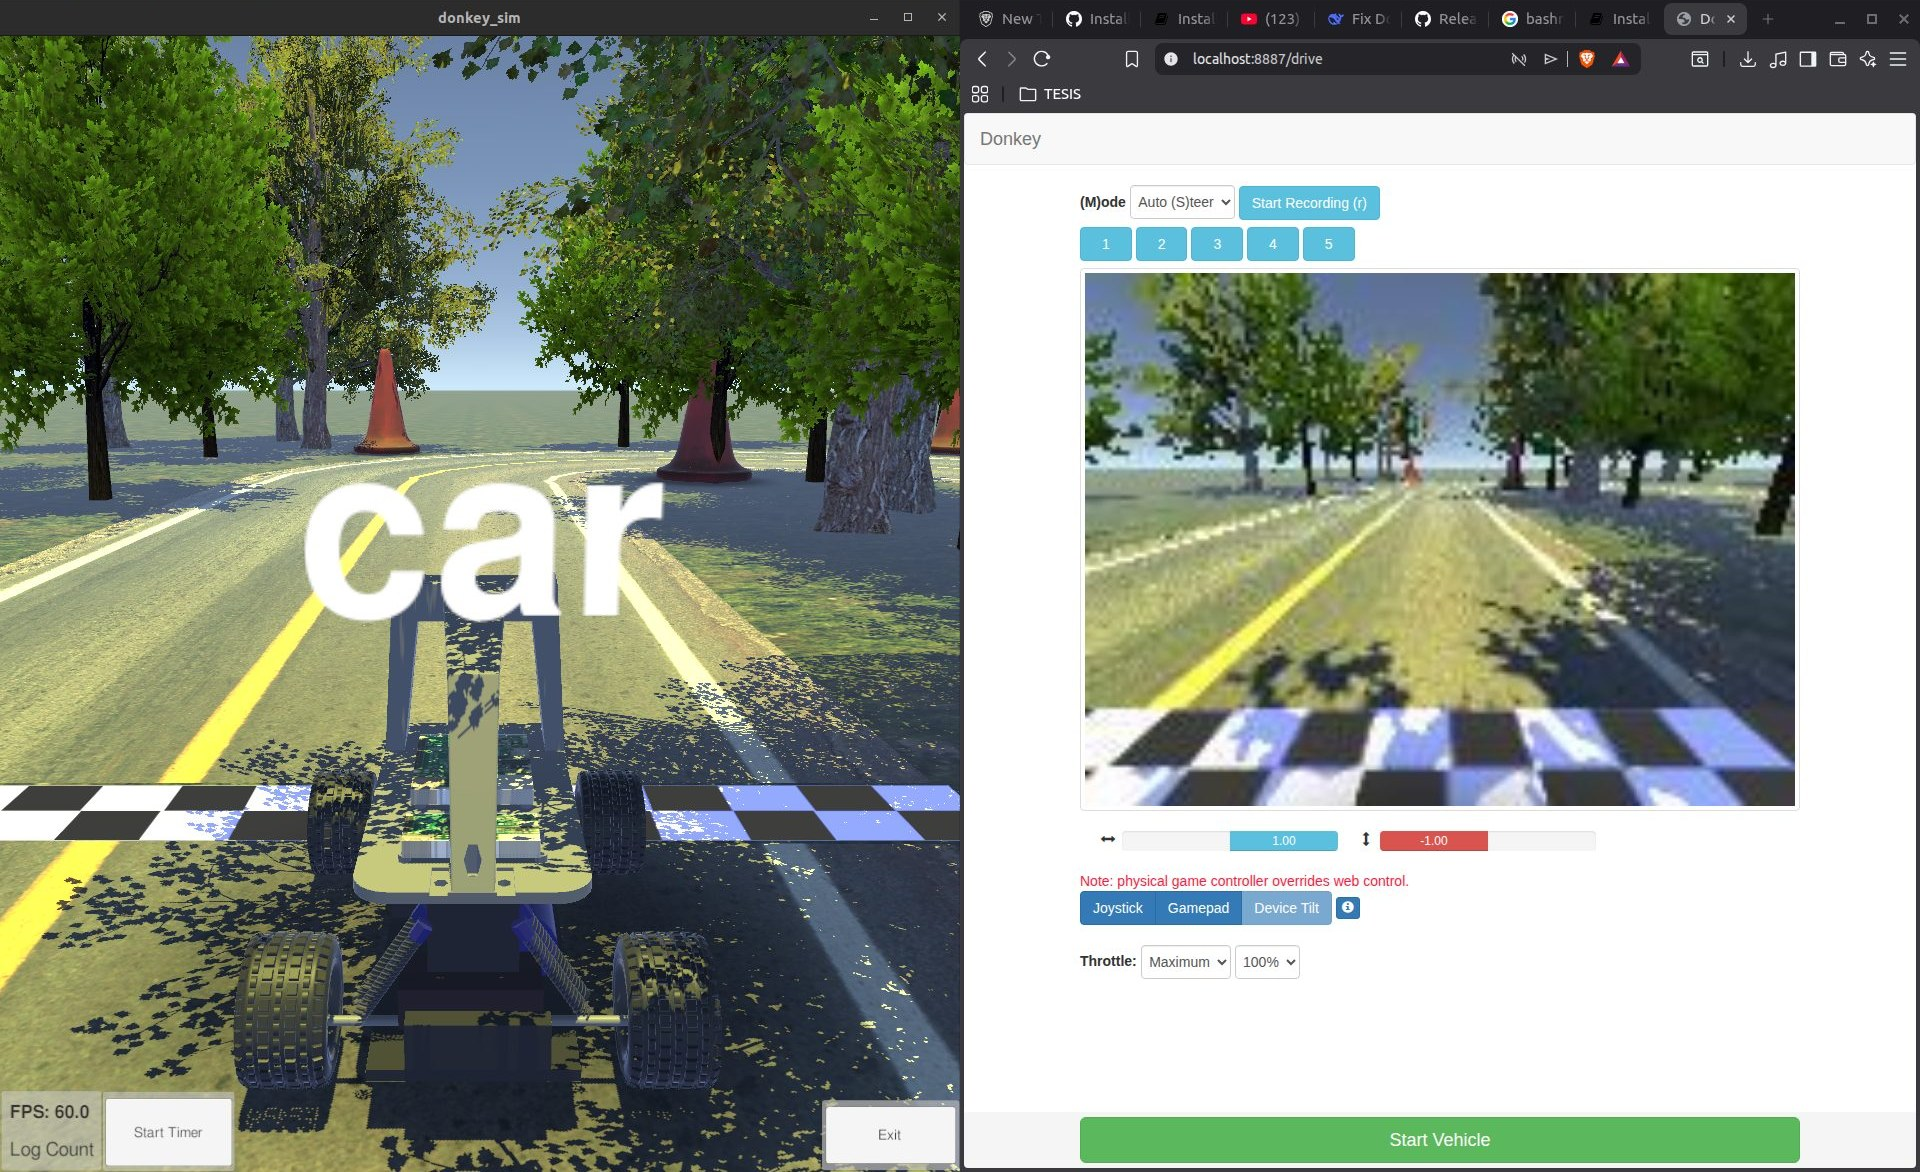
\includegraphics[height=5.2cm]{imagenes/etapa_donkeycar_simulador.jpg}\hfill
  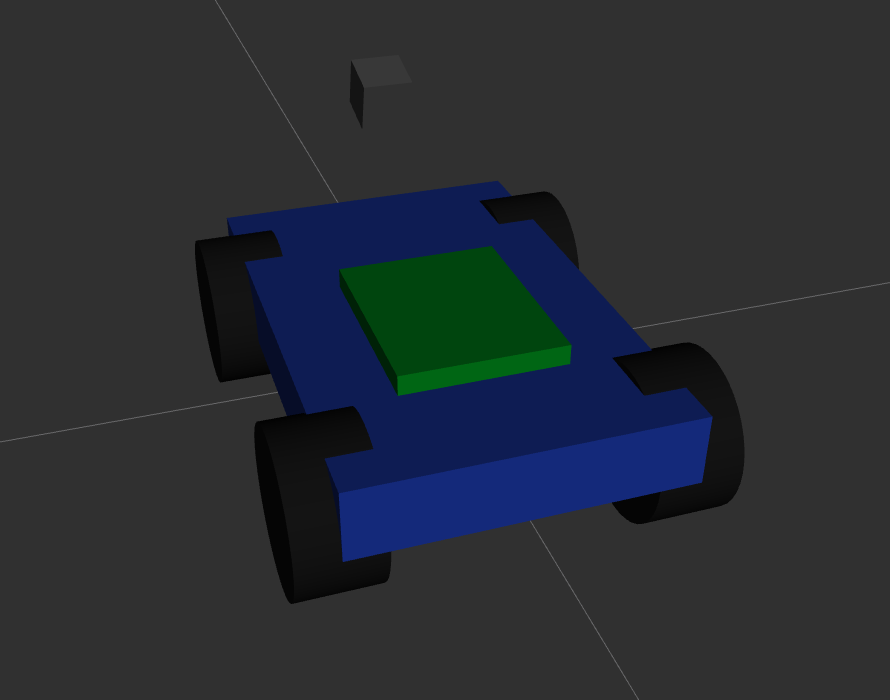
\includegraphics[height=5.2cm]{imagenes/etapa_donkeycar_modelo.png}
  \caption{Exploración de la plataforma DonkeyCar. A la izquierda, su simulador
    conducido desde la interfaz web de la plataforma, con la imagen de la cámara a bordo. A la derecha, el modelo propio del agente en el visualizador
    de ROS~2, con el chasis, las ruedas y la dirección.}
  \label{fig:donkeycar}
\end{figure}

Con ese trabajo se identificaron las limitaciones de la plataforma. El ecosistema DonkeyCar no se actualiza desde hace
años y no es compatible con las versiones recientes de ROS~2. Su simulador tampoco se comunica con ROS~2, así que no
permite probar el mapeo, la localización, la planificación ni la comunicación entre agentes, que son el núcleo del
proyecto. Además, no existía un modelo del DonkeyCar para Gazebo con dirección Ackermann que funcionara en ROS~2 Humble.

Para el simulador se fijaron cuatro criterios: compatibilidad con ROS~2 Humble, vehículos con dirección Ackermann,
entornos interiores y soporte para mapeo y navegación. Entre CoppeliaSim, que proponía el anteproyecto, el simulador del
curso F1TENTH y Gazebo \autocite{koenig2004gazebo}, se eligió Gazebo por su integración directa con ROS~2 y con su sistema
de control de articulaciones. También se conservó un chasis con dirección tipo automóvil, dado que cada agente atiende un
piso y el usuario cambia de piso por la escalera. Ningún agente tiene que entrar a un ascensor ni subir
escalones, y la vuelta dentro del pasillo puede quedar a cargo de un planificador para automóviles.

\subsection{El modelo de AWS DeepRacer y su migración a ROS~2 Humble}
\label{sec:migracion}

Ese mismo mes se cambió al modelo de AWS DeepRacer, la decisión que hizo viable el proyecto en el tiempo disponible. Es la
misma clase de plataforma que el DonkeyCar, con chasis a escala 1:18, dirección Ackermann, computador a bordo y software
abierto, y AWS publicó en código abierto su modelo de simulación, con un complemento de cinemática Ackermann para Gazebo y
los nodos que traducen las órdenes de velocidad a los servos \autocite{awsdeepracer2021}. Además, la universidad ya tenía
dos. Lo que pide el segundo objetivo, que es cinemática tipo automóvil, bajo costo y código modificable, se cumple igual con
las dos plataformas, y usar las que existían dejó el tiempo para la coordinación. El costo fue convivir con el
software del fabricante, cuyos nodos ocupan el láser, se ejecutan con el usuario administrador y publican sin espacio de
nombres.

El software de AWS estaba escrito para ROS~2 Foxy sobre Ubuntu 20.04, mientras que el proyecto trabaja con Humble sobre
Ubuntu 22.04. La migración necesitó tres cambios, todos en el sistema de control de articulaciones: la orden que activa los
controladores pasó de \texttt{start} a \texttt{active}, y el componente que publica el estado de las articulaciones cambió
de nombre y de tipo. En un mundo vacío (figura~\ref{fig:deepracer-sim}, izquierda), el modelo apareció con el láser y la
cámara publicando a 62 cuadros por segundo, con un factor de tiempo real de 1,00 y los siete controladores activos, y la
odometría registró 0,40~m/s ante una orden de 0,5~m/s.

\begin{figure}[htbp]
  \centering
  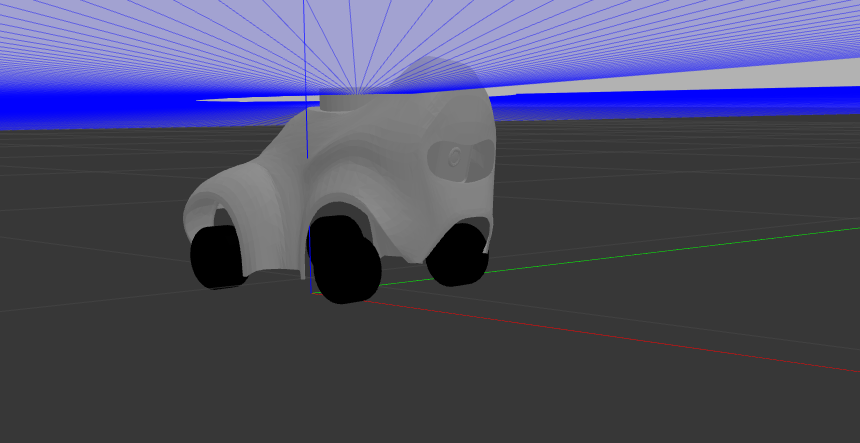
\includegraphics[height=4.6cm]{imagenes/etapa_deepracer_gazebo.png}\hfill
  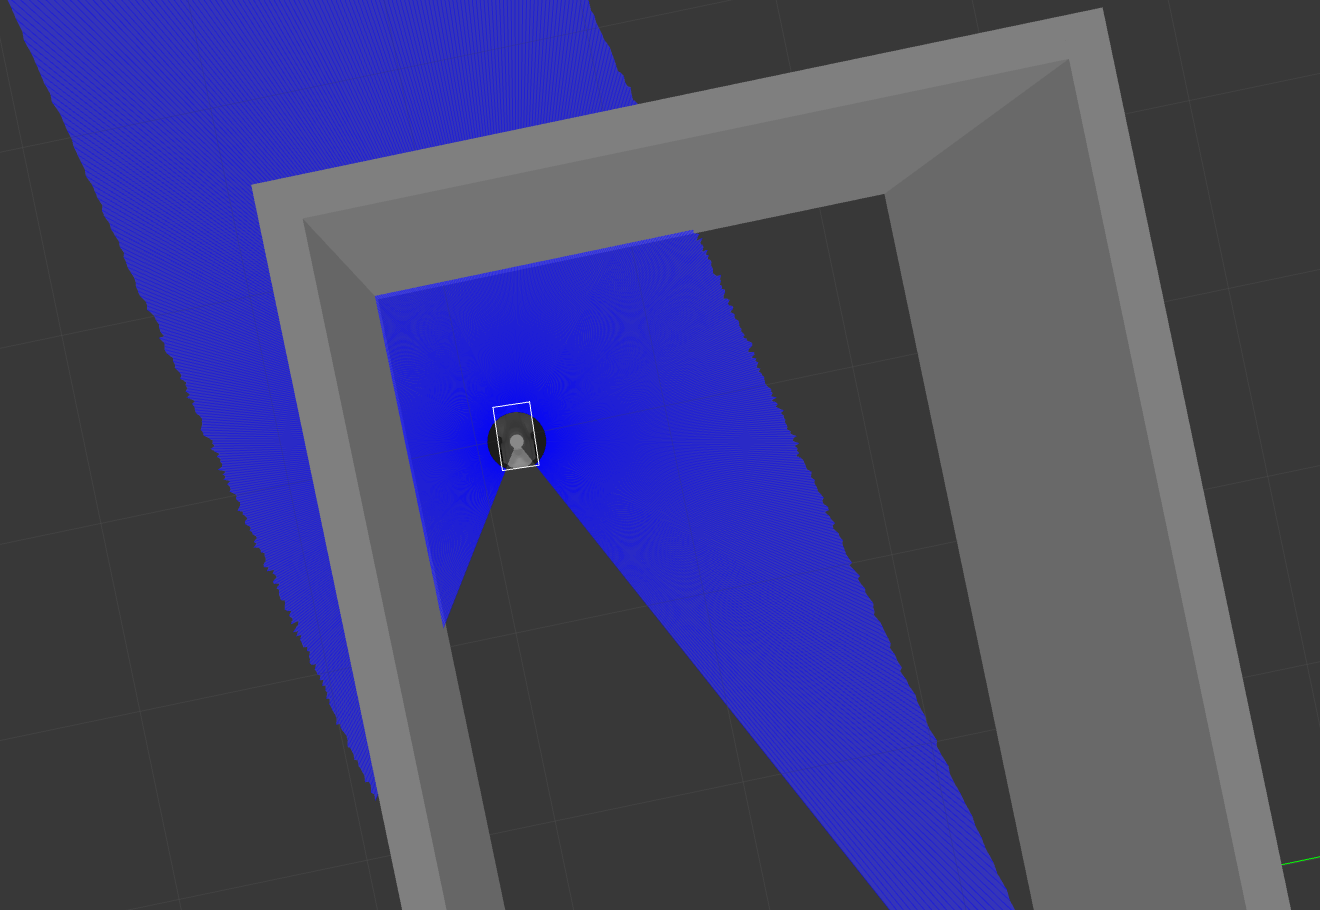
\includegraphics[height=4.6cm]{imagenes/etapa_pasillo_usta.png}
  \caption{El modelo de AWS DeepRacer migrado a ROS~2 Humble. A la izquierda, en un
    mundo vacío, con el barrido del láser en azul. A la derecha, dentro del primer
    modelo del pasillo de la universidad, de 7 por 3~m; el sector sin barrido
    detrás del agente es el que no cubría el láser del modelo simulado.}
  \label{fig:deepracer-sim}
\end{figure}

\subsection{Los primeros entornos simulados y el seguidor de paredes}
\label{sec:primeros-entornos}

En mayo se modeló un tramo del pasillo de la universidad, de 7 por 3~m (figura~\ref{fig:deepracer-sim}, derecha), y sobre
él se programó un seguidor de paredes como ejercicio de integración entre el láser y la cinemática del agente. La primera
versión aplicaba control proporcional-derivativo sobre un rayo lateral del láser, pero saturaba el giro al no conocer la
orientación del agente respecto a la pared. La segunda usó la técnica de dos rayos del curso F1TENTH, que estima ese ángulo y
la distancia a la pared un metro más adelante.

En el pasillo de 7 por 3~m ninguna sintonía estabilizó al agente: el giro se saturaba y el agente trazaba círculos o chocaba,
ya que su radio de giro deja muy poco margen en 3~m de ancho. En un pasillo ampliado de 15 por 5~m convergió por tramos, a
0,76~m de la pared frente a un objetivo de 0,5~m, y se perdía en los extremos. De estos ensayos se concluyó que un
comportamiento reactivo no anticipa las restricciones de un vehículo tipo automóvil en un pasillo estrecho, por lo que el
proyecto pasó a navegar con un mapa y con un planificador que conoce esas restricciones.

Después se modeló el primer entorno de pruebas, el piso 2 del edificio Gregorio de la universidad, donde están los salones ETM:
un pasillo de 44,25~m de largo y 5,09~m de ancho, en el que se comprobaron el láser, la cámara, la odometría y el árbol de
transformaciones. Con ese mundo se construyó el primer mapa por localización y mapeo simultáneos (SLAM), que se aceptó sin
medirlo. Al medirlo en septiembre resultó de 23,04 por 15,72~m, es decir, la mitad del largo y el triple del ancho del
pasillo. Fue la primera manifestación, sin diagnóstico entonces, de la falta de información de avance en un pasillo recto, que
acabó determinando cómo se hicieron los mapas.

\subsection{La integración en simulación}
\label{sec:recorrido-sim}

El segundo semestre empezó con un cronograma replanificado y con la revisión de la base de trabajo. El espacio de trabajo donde
se compilaba el código era una copia del repositorio del fabricante, sin enlace al del proyecto, así que los ajustes del mapeo
del primer semestre nunca se habían ejecutado. Por lo tanto, se enlazó al repositorio del proyecto y se fijó el contrato de
interfaces.

En agosto se aislaron los dos agentes, se construyó el entorno de dos pisos, con los pisos 2 y 3 del edificio Gregorio, y se
escribieron los requisitos y el protocolo. A finales de agosto se completó la primera misión con relevo, y la campaña de treinta
misiones se ejecutó el 4 y el 5 de septiembre.

También se corrigió el modelo del agente, que tomaba la velocidad angular de la orden estándar de ROS~2 como el ángulo del
volante. Desde entonces el ángulo se calcula con el modelo de bicicleta, a partir de las velocidades angular y lineal y de la
distancia entre ejes, con lo que el error de seguimiento de las trayectorias bajó a la mitad. La misma corrección se aplicó al
nodo que mueve al agente físico.

\subsection{Del primer agente físico a la campaña con los dos}
\label{sec:recorrido-fisico}

Con los agentes físicos se trabajó en paralelo desde agosto. Se instaló el software de la comunidad de AWS DeepRacer
\autocite{deepracercustomcar} en una Raspberry Pi~4 y en la tarjeta original, y los agentes quedaron con su tarjeta original, con
Ubuntu 24.04 y ROS~2 Jazzy. Como la integración de Gazebo~11 con ROS~2 no está publicada para Jazzy, desde entonces el proyecto
trabaja con dos distribuciones.

Las pruebas con los agentes físicos empezaron en los pasillos del edificio Gregorio, los mismos que se habían modelado para la
simulación. Sin embargo, allí el tránsito de personas dificultaba las pruebas, en esos pasillos uniformes la odometría del láser no
registraba el avance y el modelo del piso 3 no correspondía a la planta real. Por esa razón, el 2 de octubre el trabajo pasó a los
pisos 3 y 4 del edificio Catalayud, que el equipo levantó con flexómetro ese mismo día. De esas medidas salieron los mapas, los mundos
simulados y el catálogo de destinos de la campaña física.

Como los mundos simulados salen de las mismas medidas, el sistema también puede ejecutarse en simulación en los pisos donde operan los
agentes físicos, con un proceso de Gazebo por piso (figura~\ref{fig:sim-catalayud}). Se comprobó el 2 de noviembre, después de la
campaña, con los mismos mapas, los mismos destinos y la misma página: de trece misiones, diez se completaron, tres se cancelaron a
propósito y ninguna falló, con llegadas entre 0,067 y 0,206~m. Funcionaron además dos partes que hasta entonces solo se habían usado con
los agentes físicos, la maniobra de media vuelta y la verificación de la llegada con la posición del agente en el mapa. Fue una
comprobación de funcionamiento, sin el protocolo de la campaña, que no entra en sus resultados. La simulación sigue sin reproducir lo
físico: la odometría real, la respuesta de la tracción y la red entre pisos.

\begin{figure}[htbp]
  \centering
  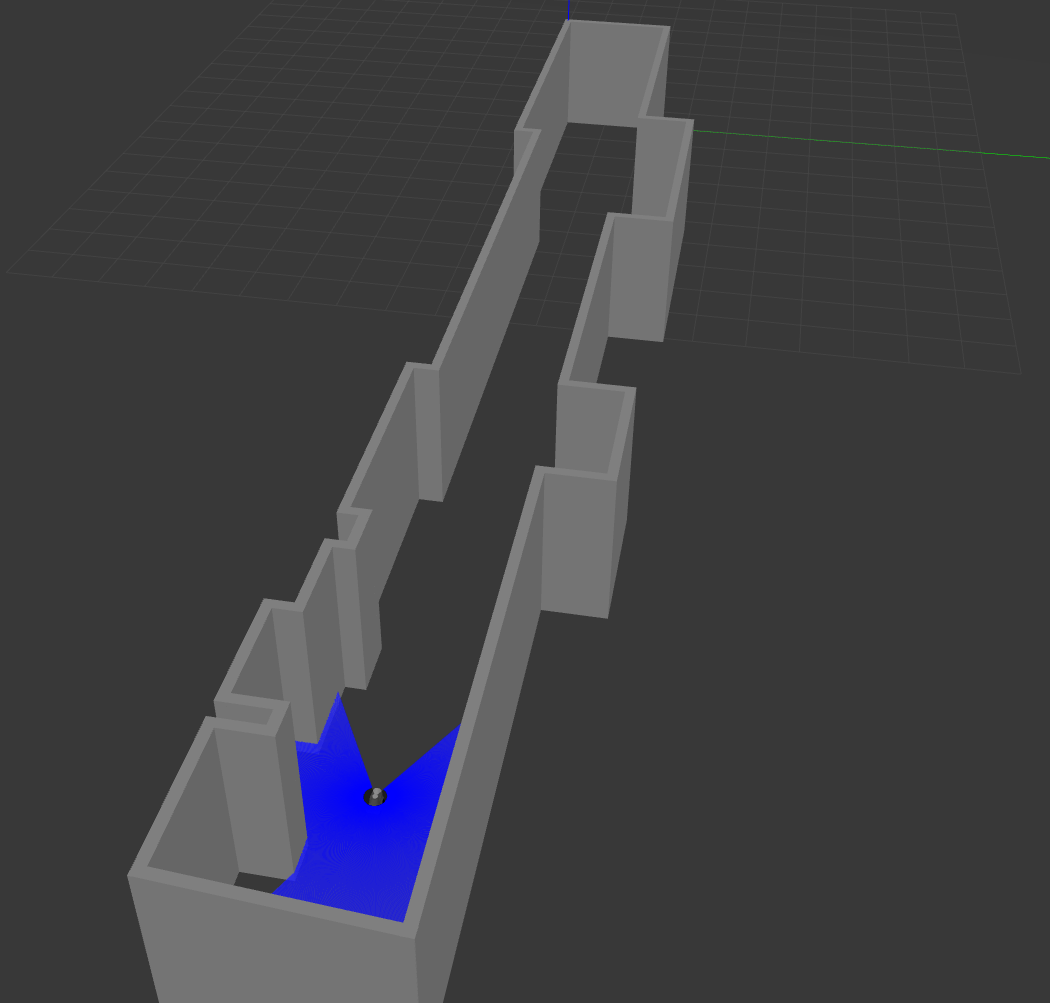
\includegraphics[width=0.49\textwidth]{imagenes/simulacion_catalayud_piso3.png}\hfill
  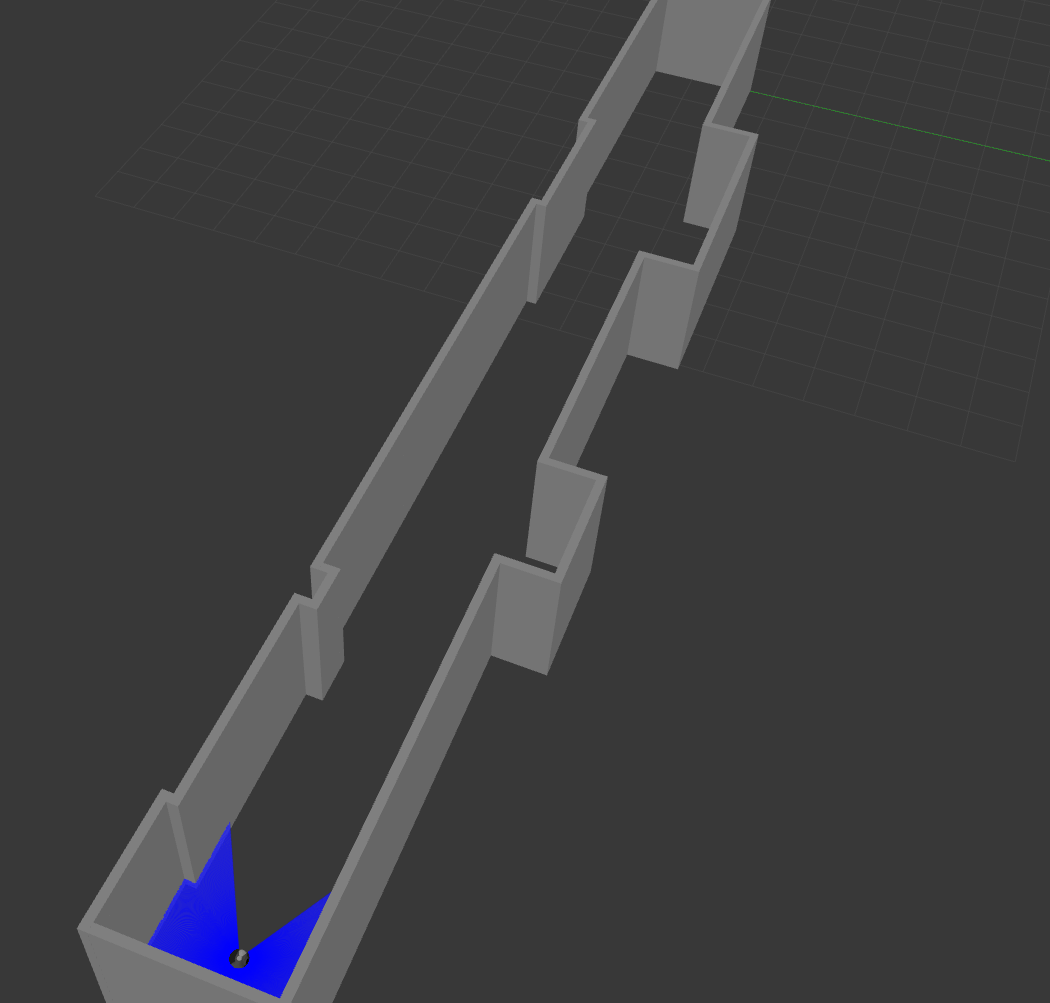
\includegraphics[width=0.49\textwidth]{imagenes/simulacion_catalayud_piso4.png}
  \caption{Los pisos 3 (izquierda) y 4 (derecha) del edificio Catalayud en simulación, cada uno en su proceso de Gazebo. Cada agente está en su salida, frente a la escalera, con el barrido del láser en azul.}
  \label{fig:sim-catalayud}
\end{figure}

El 21 de septiembre se decidió intentar la demostración física con seis pruebas de verificación, y la campaña con los agentes físicos se ejecutó el 16 de octubre.

% =====================================================================
\section{Arquitectura funcional del sistema}
\label{sec:oe1}

La figura~\ref{fig:arquitectura} muestra el sistema tal como se implementó en
simulación: la interfaz por la que entra la solicitud, el coordinador que la
reparte, los dos agentes con su pila de navegación y la escalera donde ocurre el
relevo.

\begin{figure}[htbp]
  \centering
  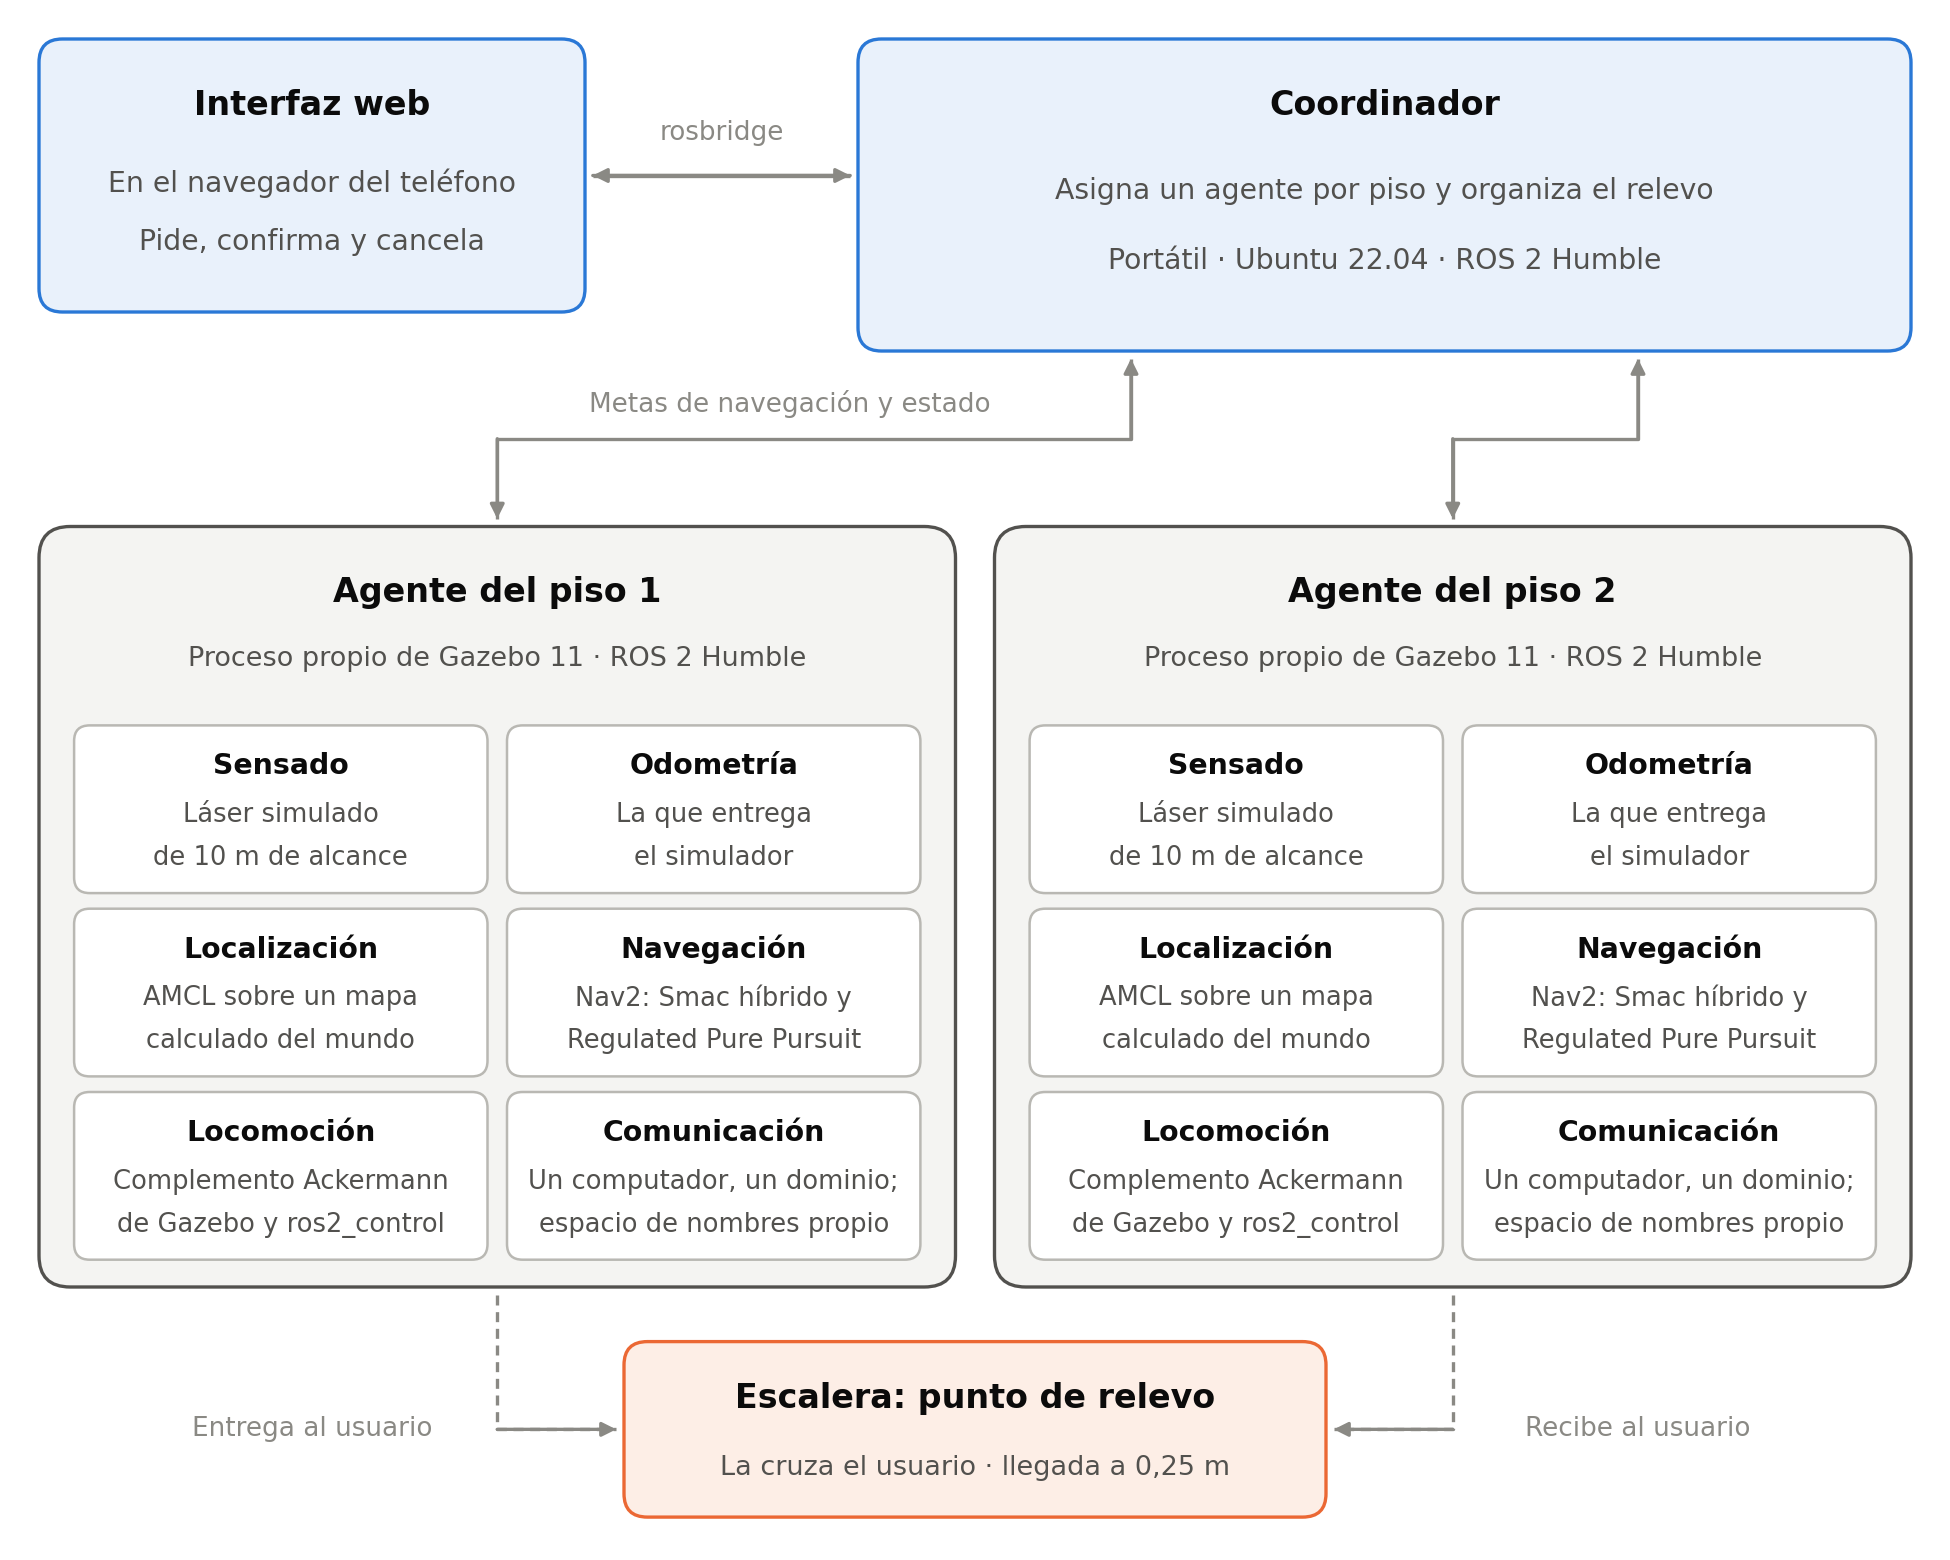
\includegraphics[width=0.86\textwidth]{imagenes/arquitectura_simulacion.png}
  \caption{Arquitectura del sistema en simulación, con un proceso de Gazebo por
    piso. Ningún agente atraviesa la zona de transición: lo que la cruza es el
    usuario, y lo que se traspasa entre agentes es la responsabilidad de guiarlo.}
  \label{fig:arquitectura}
\end{figure}

\subsection{Requisitos}

El anteproyecto no enumeró los requisitos del sistema, aunque su metodología pedía verificar la implementación contra ellos. Por ello,
se reconstruyeron al iniciar la integración a partir de los objetivos específicos, el alcance y el contrato de interfaces. Cada requisito
cita su fuente y tiene una prueba que lo declara cumplido o no; un requisito sin prueba no entra en la matriz.

La matriz tiene treinta y seis requisitos: veintinueve describen funciones del
sistema y siete son restricciones del alcance, como operar en interiores y en
condiciones controladas o ejecutar la simulación en tiempo real. Al primer objetivo
le corresponden diez, sobre arquitectura, coordinación y relevo; al segundo,
seis, sobre la plataforma; al tercero, seis, sobre la interfaz; y al cuarto, siete,
sobre las métricas, el registro de cada misión y las dos campañas. La confirmación de cambio de piso y la cancelación no estaban en el anteproyecto: se añadieron al ver el sistema en uso. El avance de cada objetivo es el
promedio del estado de sus requisitos.

\subsection{El contrato de interfaces}
\label{sec:contrato}

Antes de escribir código se fijó un contrato que define qué habla con qué y en qué formato. Un coordinador decide y manda, dos agentes, uno
por piso, ejecutan, y una interfaz web es la vía por la que el usuario pide el servicio. La comunicación sigue tres reglas:

\begin{enumerate}[leftmargin=*]
  \item El coordinador manda a un agente solo mediante la acción de navegación
    de ROS~2; no publica velocidades directamente. En la versión final puede
    pedirle además una media vuelta, que el agente ejecuta por su cuenta antes de navegar.
  \item La interfaz habla solo con el coordinador, nunca con los agentes.
  \item El texto que ve el usuario lo redacta el coordinador, y la interfaz lo
    muestra literal.
\end{enumerate}

La tercera regla evita duplicar la lógica: si la página interpretara el estado para decidir qué mostrar, habría dos copias de la misma lógica, que con el tiempo acabarían contradiciéndose.

El contrato se implementó como un paquete propio de mensajes de ROS~2. La acción
de guiado recibe el origen y el destino, devuelve el estado durante la misión y,
al final, el tiempo total y el número de relevos o el motivo del fallo. Cada
cambio de etapa (tabla~\ref{tab:etapas-mision}) se publica, y esas publicaciones
son las marcas de tiempo con que se calculan las métricas. La tabla~\ref{tab:contrato} reúne las interfaces entre los componentes, y la figura~\ref{fig:nodos} muestra los nodos principales del sistema en la campaña con los agentes físicos y lo que circula entre ellos. El anexo C trae el grafo completo, obtenido en simulación.

\begin{table}[!htbp]
  \centering\footnotesize
  \caption{Interfaces del contrato entre la interfaz web, el coordinador y los agentes. \texttt{N} es el número del agente: 1 en el piso inferior y 2 en el superior.}
  \label{tab:contrato}
  \begin{tabular}{@{}p{0.36\textwidth}p{0.16\textwidth}p{0.13\textwidth}p{0.27\textwidth}@{}}
    \toprule
    \textbf{Interfaz} & \textbf{Tipo} & \textbf{Sentido} & \textbf{Contenido} \\ \midrule
    \texttt{/coordinacion/guiar\_usuario} & acción propia & interfaz $\rightarrow$ coordinador & Origen y destino; devuelve el estado durante la misión y, al final, el éxito, el tiempo total, los relevos o el motivo del fallo \\ \addlinespace
    \texttt{/coordinacion/estado\_mision} & tópico propio, 1~Hz & coordinador $\rightarrow$ interfaz & Etapa, agente activo, destino del tramo, distancia restante y texto para el usuario \\ \addlinespace
    \texttt{/coordinacion/puntos\_interes} & tópico propio, persistente & coordinador $\rightarrow$ interfaz & Catálogo de puntos de interés, con su piso \\ \addlinespace
    \texttt{/coordinacion/confirmacion\_piso} & tópico de texto & interfaz $\rightarrow$ coordinador & Confirmación de que el usuario ya cambió de piso \\ \addlinespace
    \texttt{/robotN/navigate\_to\_pose} & acción de Nav2 & coordinador $\rightarrow$ agente & Meta de cada tramo; es la única orden de movimiento \\ \addlinespace
    \texttt{/robotN/media\_vuelta} & servicio & coordinador $\rightarrow$ agente & Media vuelta antes de una meta que queda detrás \\ \addlinespace
    \texttt{/robotN/estado} & tópico propio, 2~Hz & agente $\rightarrow$ coordinador & Piso, pose en el mapa y estado del agente \\ \addlinespace
    \texttt{/robotN/odom} & odometría & agente $\rightarrow$ coordinador & Desplazamiento, con el que se marca el primer movimiento \\ \bottomrule
  \end{tabular}
\end{table}

\begin{figure}[!htbp]
  \centering
  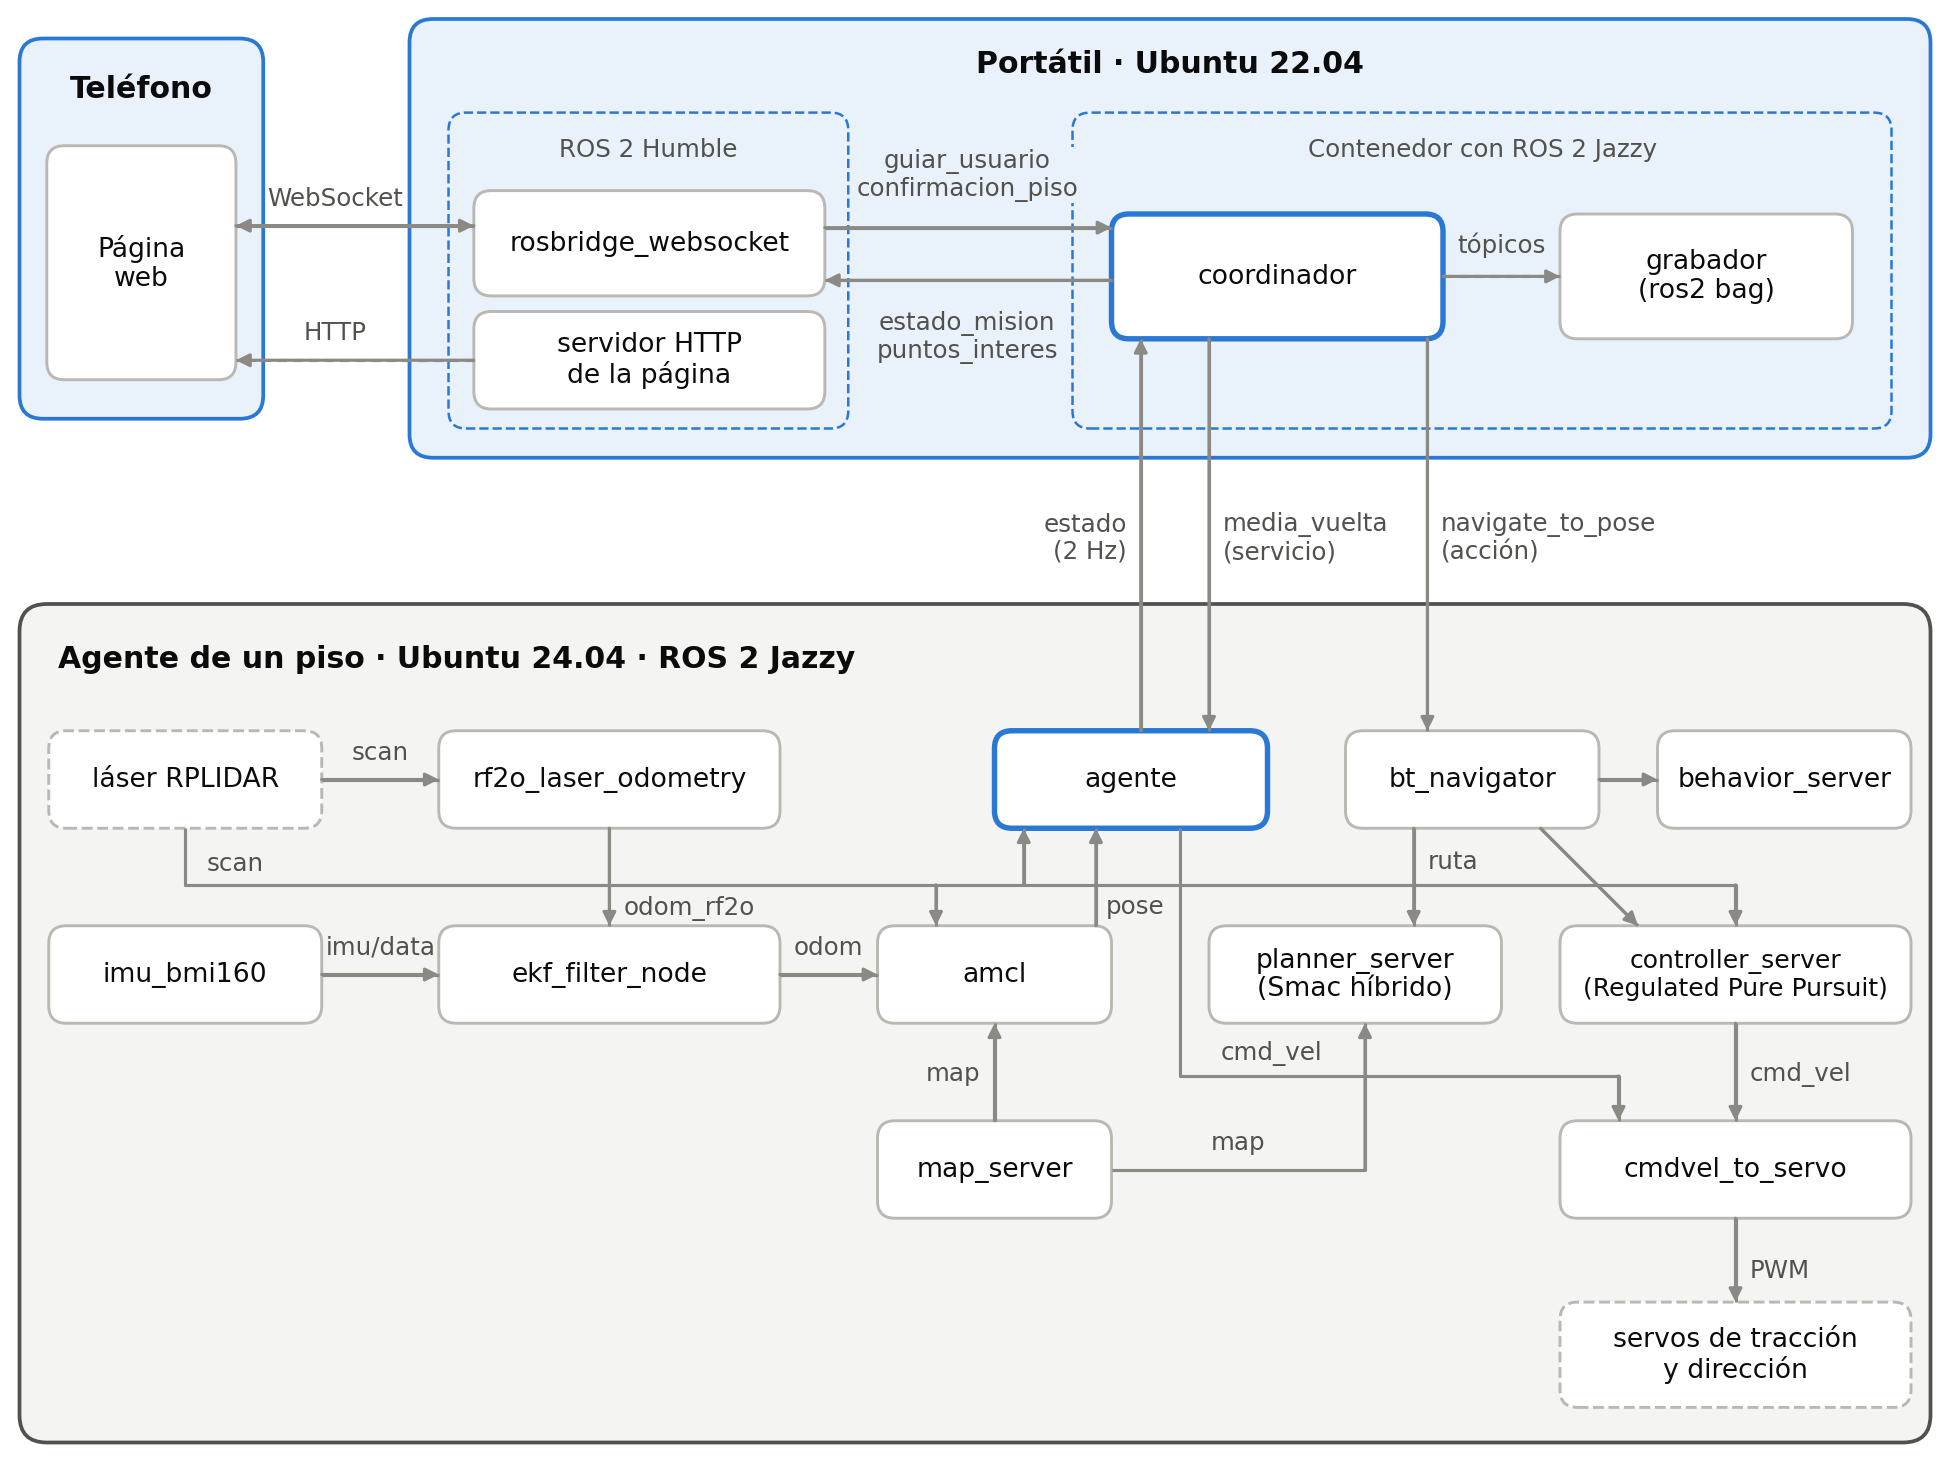
\includegraphics[width=0.96\textwidth]{imagenes/nodos_sistema.png}
  \caption{Nodos principales de ROS~2 del sistema en la campaña con los agentes físicos. Los dos agentes son iguales; en borde discontinuo, los componentes del fabricante. Las flechas siguen el sentido de los datos y llevan el nombre del tópico, servicio o acción. El navegador pide la ruta al planificador y su seguimiento al controlador, y la pose que estima \texttt{amcl} llega a los demás nodos por las transformadas.}
  \label{fig:nodos}
\end{figure}

\begin{table}[htbp]
  \centering\small
  \caption{Etapas de una misión, tal como las publica el coordinador.}
  \label{tab:etapas-mision}
  \begin{tabular}{@{}p{0.27\textwidth}p{0.65\textwidth}@{}}
    \toprule
    \textbf{Etapa} & \textbf{Significado} \\ \midrule
    Recibida & El coordinador aceptó la solicitud y todavía no asignó agente \\
    Primer tramo & El agente del piso de origen va a recoger al usuario y lo guía \\
    Transferencia & El agente del otro piso va a su punto de transferencia \\
    Esperando confirmación & El sistema espera que el usuario confirme que ya cambió de piso \\
    Segundo tramo & El agente del piso de destino guía al usuario hasta el final \\
    Completada & La misión terminó con la llegada verificada \\
    Fallida & La misión terminó sin cumplirse, con el motivo en el texto \\
    Cancelando & El usuario canceló y el agente activo regresa a su punto de transferencia \\
    Inactiva & No hay misión en curso \\ \bottomrule
  \end{tabular}
\end{table}

\subsection{El planificador, escrito sin ROS}
\label{sec:planificador}

El relevo es el aporte declarado del proyecto, y por esa razón su planificación se escribió como una función pura, sin dependencia de ROS~2 ni
estado propio (figura~\ref{fig:planificador}). Entran el catálogo de puntos y un par origen-destino, y salen los tramos que hay que ejecutar. Si
el origen y el destino están en el mismo piso, la misión tiene dos tramos del mismo agente: ir a recoger al usuario y llevarlo al destino. Si
están en pisos distintos, tiene cuatro: los dos anteriores, terminando en el punto de transferencia del piso de origen; el desplazamiento del
segundo agente a su punto de transferencia; y el guiado final. El punto de encuentro no se negocia: es el punto de transferencia declarado
de cada piso en el catálogo.

\begin{figure}[!htbp]
  \centering
  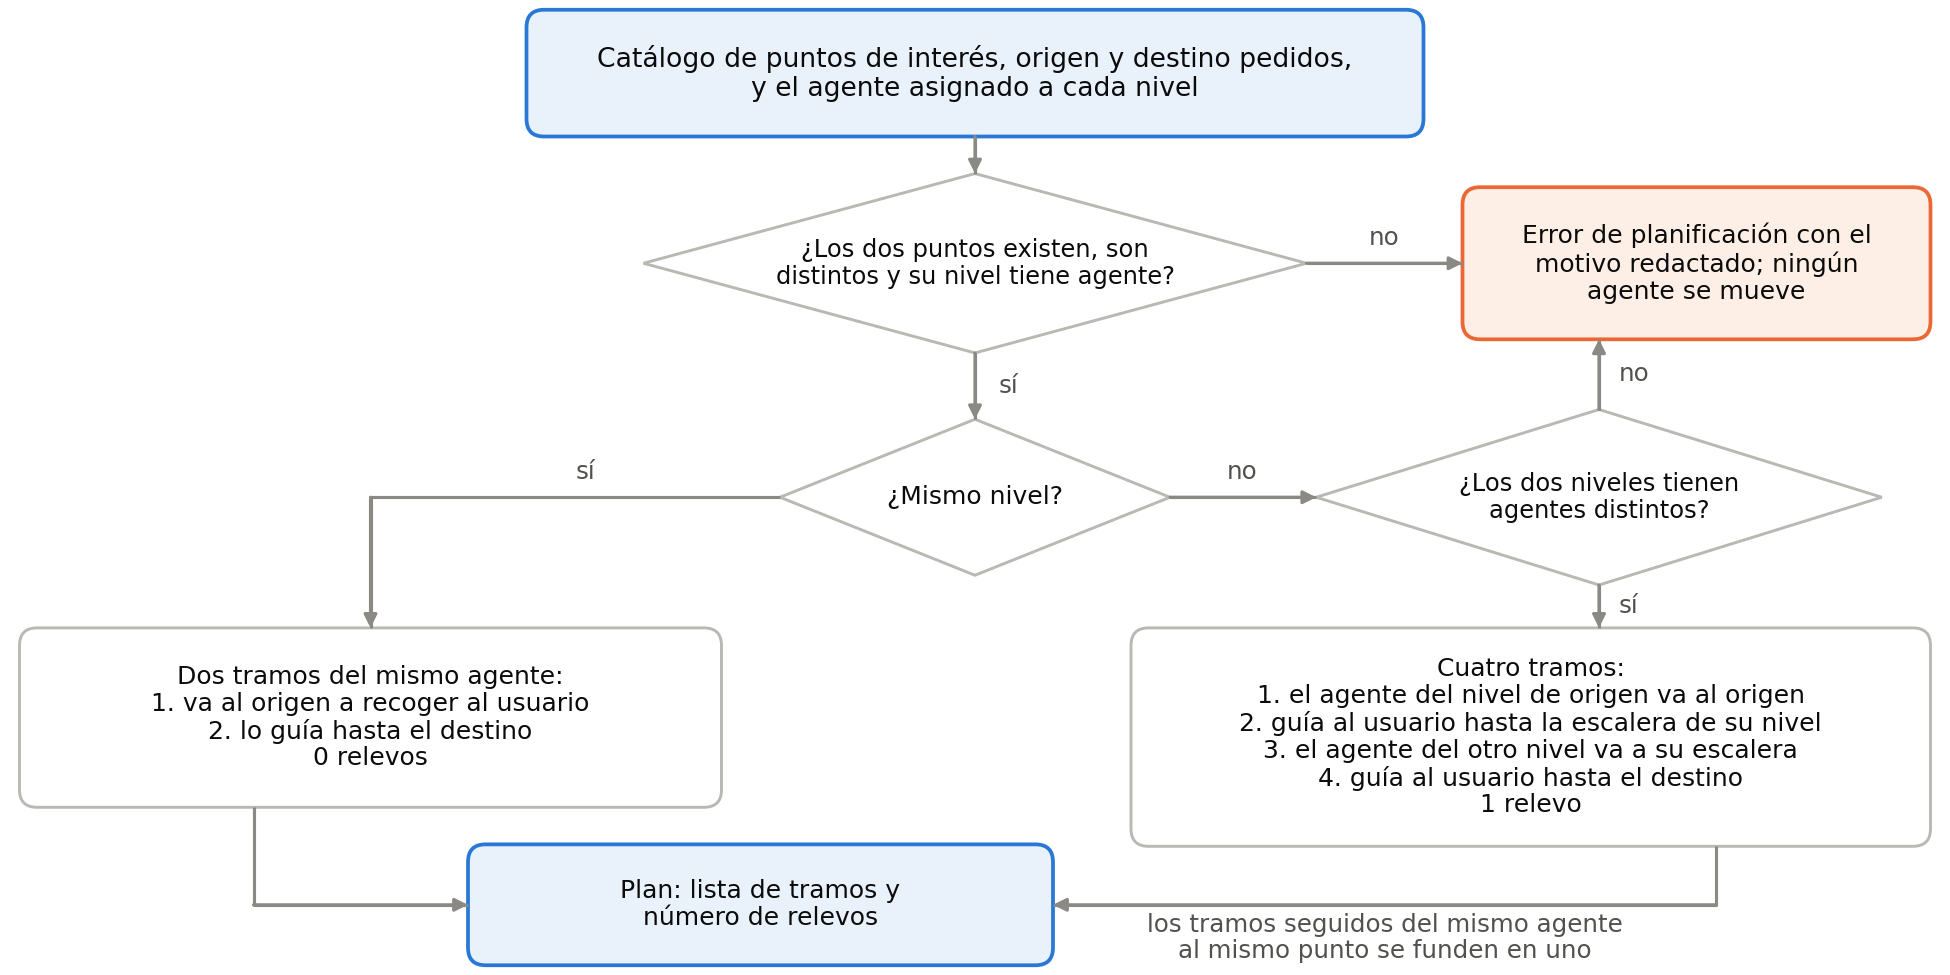
\includegraphics[width=0.84\textwidth]{imagenes/planificador.png}
  \caption{Función que planifica una misión. No usa ROS~2: recibe el catálogo, el origen, el destino y la asignación de un agente por piso, y devuelve la lista de tramos o un error con su motivo, antes de que ningún agente se mueva.}
  \label{fig:planificador}
\end{figure}

Con el relevo dentro del nodo, mezclado con los clientes de acción, la única forma de comprobarlo habría sido levantar dos simuladores y observar si
el agente llega. Como función pura, en cambio, una prueba automática la recorre entera en milisegundos y sin simulador. El catálogo de la simulación
tiene 31 puntos de interés, y cada par ordenado de dos puntos distintos es una solicitud posible: $31 \times 30 = 930$ combinaciones de origen y
destino. La prueba planifica las 930 y comprueba en todas que el plan empieza en el origen y termina en el destino y que ningún agente recibe una
meta fuera de su piso, además de que una misión de un solo piso usa un agente y ningún relevo, y una de dos pisos usa los dos agentes y un relevo. Con
esa prueba se encontró un defecto que una ejecución no habría mostrado: cuando el origen o el destino era el propio punto de transferencia de su piso,
el plan mandaba al mismo agente dos veces a la misma pose, y como Nav2 devuelve éxito al instante ante un desplazamiento de cero metros, en simulación
no se habría visto.

\subsection{La asignación de tareas}
\label{sec:asignacion}

Cada piso tiene un agente asignado, y esa correspondencia es un dato de configuración, sin estar fija en el código. El coordinador elige el agente al
aceptar la solicitud, según el piso del origen y del destino.

El planificador exige un único punto de transferencia por piso y falla con un mensaje explícito si encuentra dos. Como cada piso tiene una escalera, la
condición se cumple, y la verificación obliga a tomar la decisión a la vista si algún día hubiera dos. En los agentes físicos, además, el coordinador
comprueba la llegada con la pose que publica el agente, sin darla por buena solo porque Nav2 la informe.

\subsection{Escenarios de operación en simulación}
\label{sec:simulacion}

Los escenarios de varios pisos se construyeron primero en Gazebo~11 con ROS~2 Humble. La integración de Gazebo con ROS~2 en Humble aplica a todos los
complementos el espacio de nombres del primer modelo cargado, lo que impidió tener dos agentes en un mismo proceso, y cada uno tiene su propio
simulador. El catálogo llegó a 31 puntos de interés: quince en el piso 2 y dieciséis en el piso 3 del edificio Gregorio.

Al principio los dos pisos estaban en un mismo mundo, y el láser simulado, de 10~m de alcance, veía paredes del otro piso en 61 de 1701 posiciones muestreadas,
justo donde arranca el primer agente y donde está su punto de transferencia. Por esa razón, cada piso pasó a ser un mundo distinto, con su propio proceso de
simulación. Los dos agentes comparten un dominio de comunicaciones, separados por espacio de nombres, y la figura~\ref{fig:sim-relevo} muestra una misión con
relevo entre los dos procesos.

\begin{figure}[htbp]
  \centering
  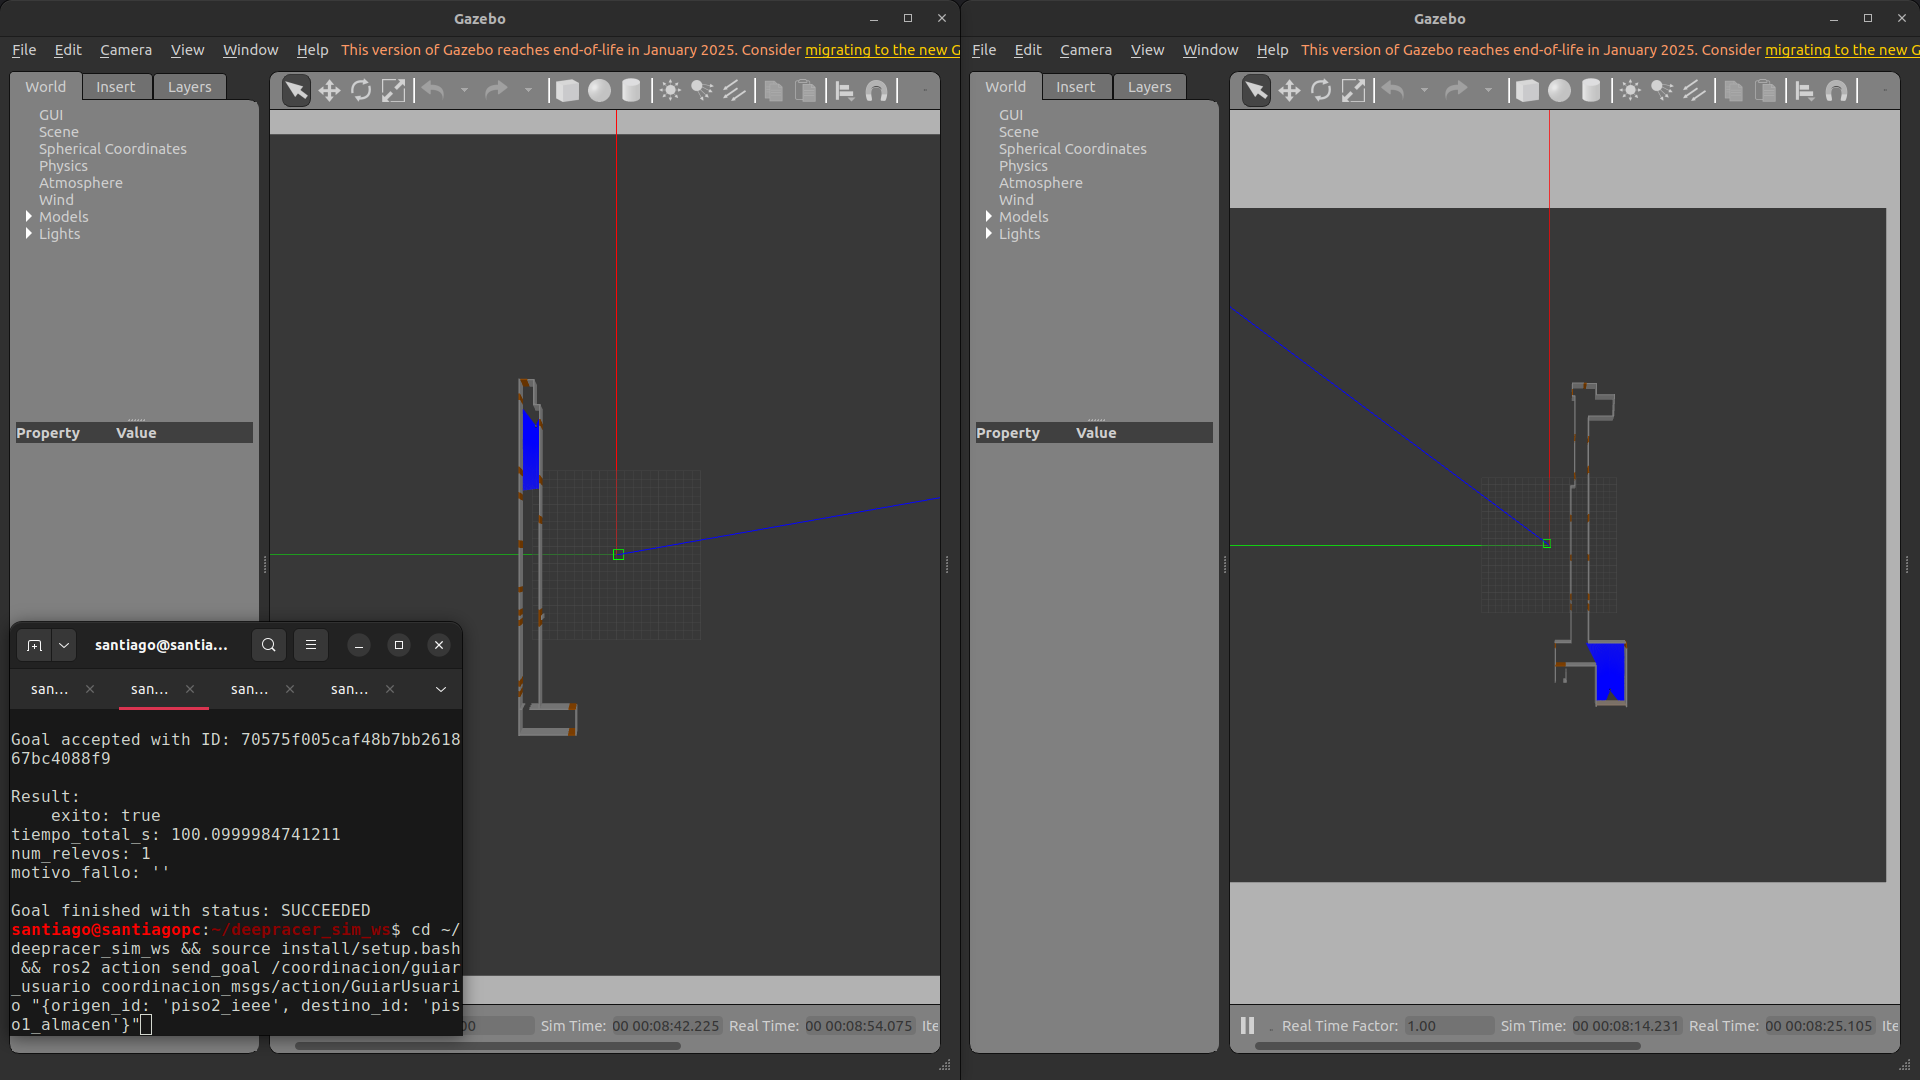
\includegraphics[width=\textwidth]{imagenes/simulacion_relevo_dos_procesos.png}
  \caption{Misión con relevo en simulación. Cada ventana es un proceso de Gazebo
    con un piso y su agente; el láser de cada uno se ve en azul. La terminal
    muestra el resultado de la acción: éxito, un relevo y 100,1~s de duración.}
  \label{fig:sim-relevo}
\end{figure}

El mapa de navegación tampoco salió de SLAM. Otro mapa construido con ese método, medido el 11 de agosto, cubría el 35,5~\% del largo del pasillo, medía 15,0~m de
ancho frente a los 5,3~m del mundo simulado, y 2688 de sus 3618 celdas ocupadas, el 74~\%, no tenían ninguna pared detrás. Se reemplazó por un mapa calculado de la
geometría del modelo, exacto en simulación; como un mapa de ocupación es un corte horizontal, el del piso superior resultó idéntico. Por último, la simulación debe
ejecutarse a tiempo real para que las métricas temporales valgan, y en las treinta misiones de la campaña el factor de tiempo real tuvo un mínimo de 0,9917 y una media
de 0,9973.

\subsection{De la simulación a los agentes físicos}
\label{sec:sim-a-vehiculos}

Al llevar el sistema a los agentes físicos se mantuvieron su estructura (un coordinador, un agente por piso, el relevo en la escalera y las reglas del contrato) y su
código. El del coordinador, el del planificador, el de los mensajes y el de la página es el mismo en los dos destinos: compila sin cambios en las dos distribuciones de
ROS~2 y completó una misión en cada uno. Lo que cambió fue la implementación de los bloques. La tabla~\ref{tab:sim-vehiculos} reúne cada cambio con su causa, y la
figura~\ref{fig:arquitectura-vehiculos} muestra el sistema como funcionó en la campaña con los agentes físicos.

\begin{table}[htbp]
  \centering\footnotesize
  \caption{Cambios en la implementación al pasar de la simulación a los agentes físicos.}
  \label{tab:sim-vehiculos}
  \begin{tabular}{@{}p{0.13\textwidth}p{0.21\textwidth}p{0.27\textwidth}p{0.31\textwidth}@{}}
    \toprule
    \textbf{Parte} & \textbf{En simulación} & \textbf{En los agentes físicos} & \textbf{Causa} \\ \midrule
    Distribución de ROS~2 & Humble en todos los componentes & Jazzy en los agentes y en el coordinador, que se ejecuta en un contenedor del portátil; Humble en la página y en rosbridge & El software de la tarjeta original solo existe para Ubuntu 24.04 con Jazzy, la simulación no existe en Jazzy, y la acción de navegación de Jazzy no es compatible con la de Humble \\ \addlinespace
    Coordinador & En el portátil, junto a los dos simuladores & En el portátil, después de un intento en uno de los agentes & Con el coordinador y el grabador en una tarjeta y las dos navegaciones encendidas, la carga subió de 6 a entre 17 y 33 y Nav2 no arrancaba \\ \addlinespace
    Comunicación & Un solo computador y un dominio de comunicaciones; un espacio de nombres por agente & Red inalámbrica con un punto de acceso de 5~GHz por piso; una partición por agente y topología en estrella hacia el portátil & Los tópicos del fabricante no llevan espacio de nombres, y los procesos de las dos cadenas, anunciándose por la red, saturaban las tarjetas \\ \addlinespace
    Locomoción & Complemento Ackermann de Gazebo con \texttt{ros2\_control} & Puente de la orden de velocidad a los servos, con una escala por agente & La tracción real tiene banda muerta y funciona en lazo abierto \\ \addlinespace
    Sensado & Láser simulado de 10~m de alcance & RPLIDAR A1M8 y la unidad inercial de la tarjeta; cámaras apagadas & Las cámaras no se usan y cargaban la tarjeta \\ \addlinespace
    Odometría & La del simulador & La del láser, combinada con la unidad inercial mediante un filtro & El agente no tiene codificadores en las ruedas, y con el láser solo el rumbo derivaba 5,9$^\circ$ por minuto \\ \addlinespace
    Mapa & Calculado de la geometría del mundo simulado & Derivado de la planta medida con flexómetro & El mapeo con SLAM a bordo no dio un mapa utilizable en ningún pasillo \\ \addlinespace
    Escenario & Pisos 2 y 3 del edificio Gregorio & Pisos 3 y 4 del edificio Catalayud, levantados con flexómetro & En Gregorio el tránsito de personas dificultaba las pruebas, el modelo no correspondía a la planta real y en sus pasillos uniformes la odometría del láser no veía el avance \\ \addlinespace
    Llegada & Tolerancia de 0,25~m & Tolerancia de 0,5~m, verificada con la pose del agente 1,5~s después de que Nav2 da la meta por alcanzada & Por la banda muerta, el agente no alcanza la precisión de la simulación, y sigue rodando cuando Nav2 declara la llegada \\ \addlinespace
    Media vuelta & La planifica Nav2, con marcha atrás & Maniobra propia del agente, vigilada con el láser y el mapa & En la salida del piso 4, de 2,5~m de ancho, la media vuelta de Nav2 abortó contra la pared \\ \bottomrule
  \end{tabular}
\end{table}

\begin{figure}[htbp]
  \centering
  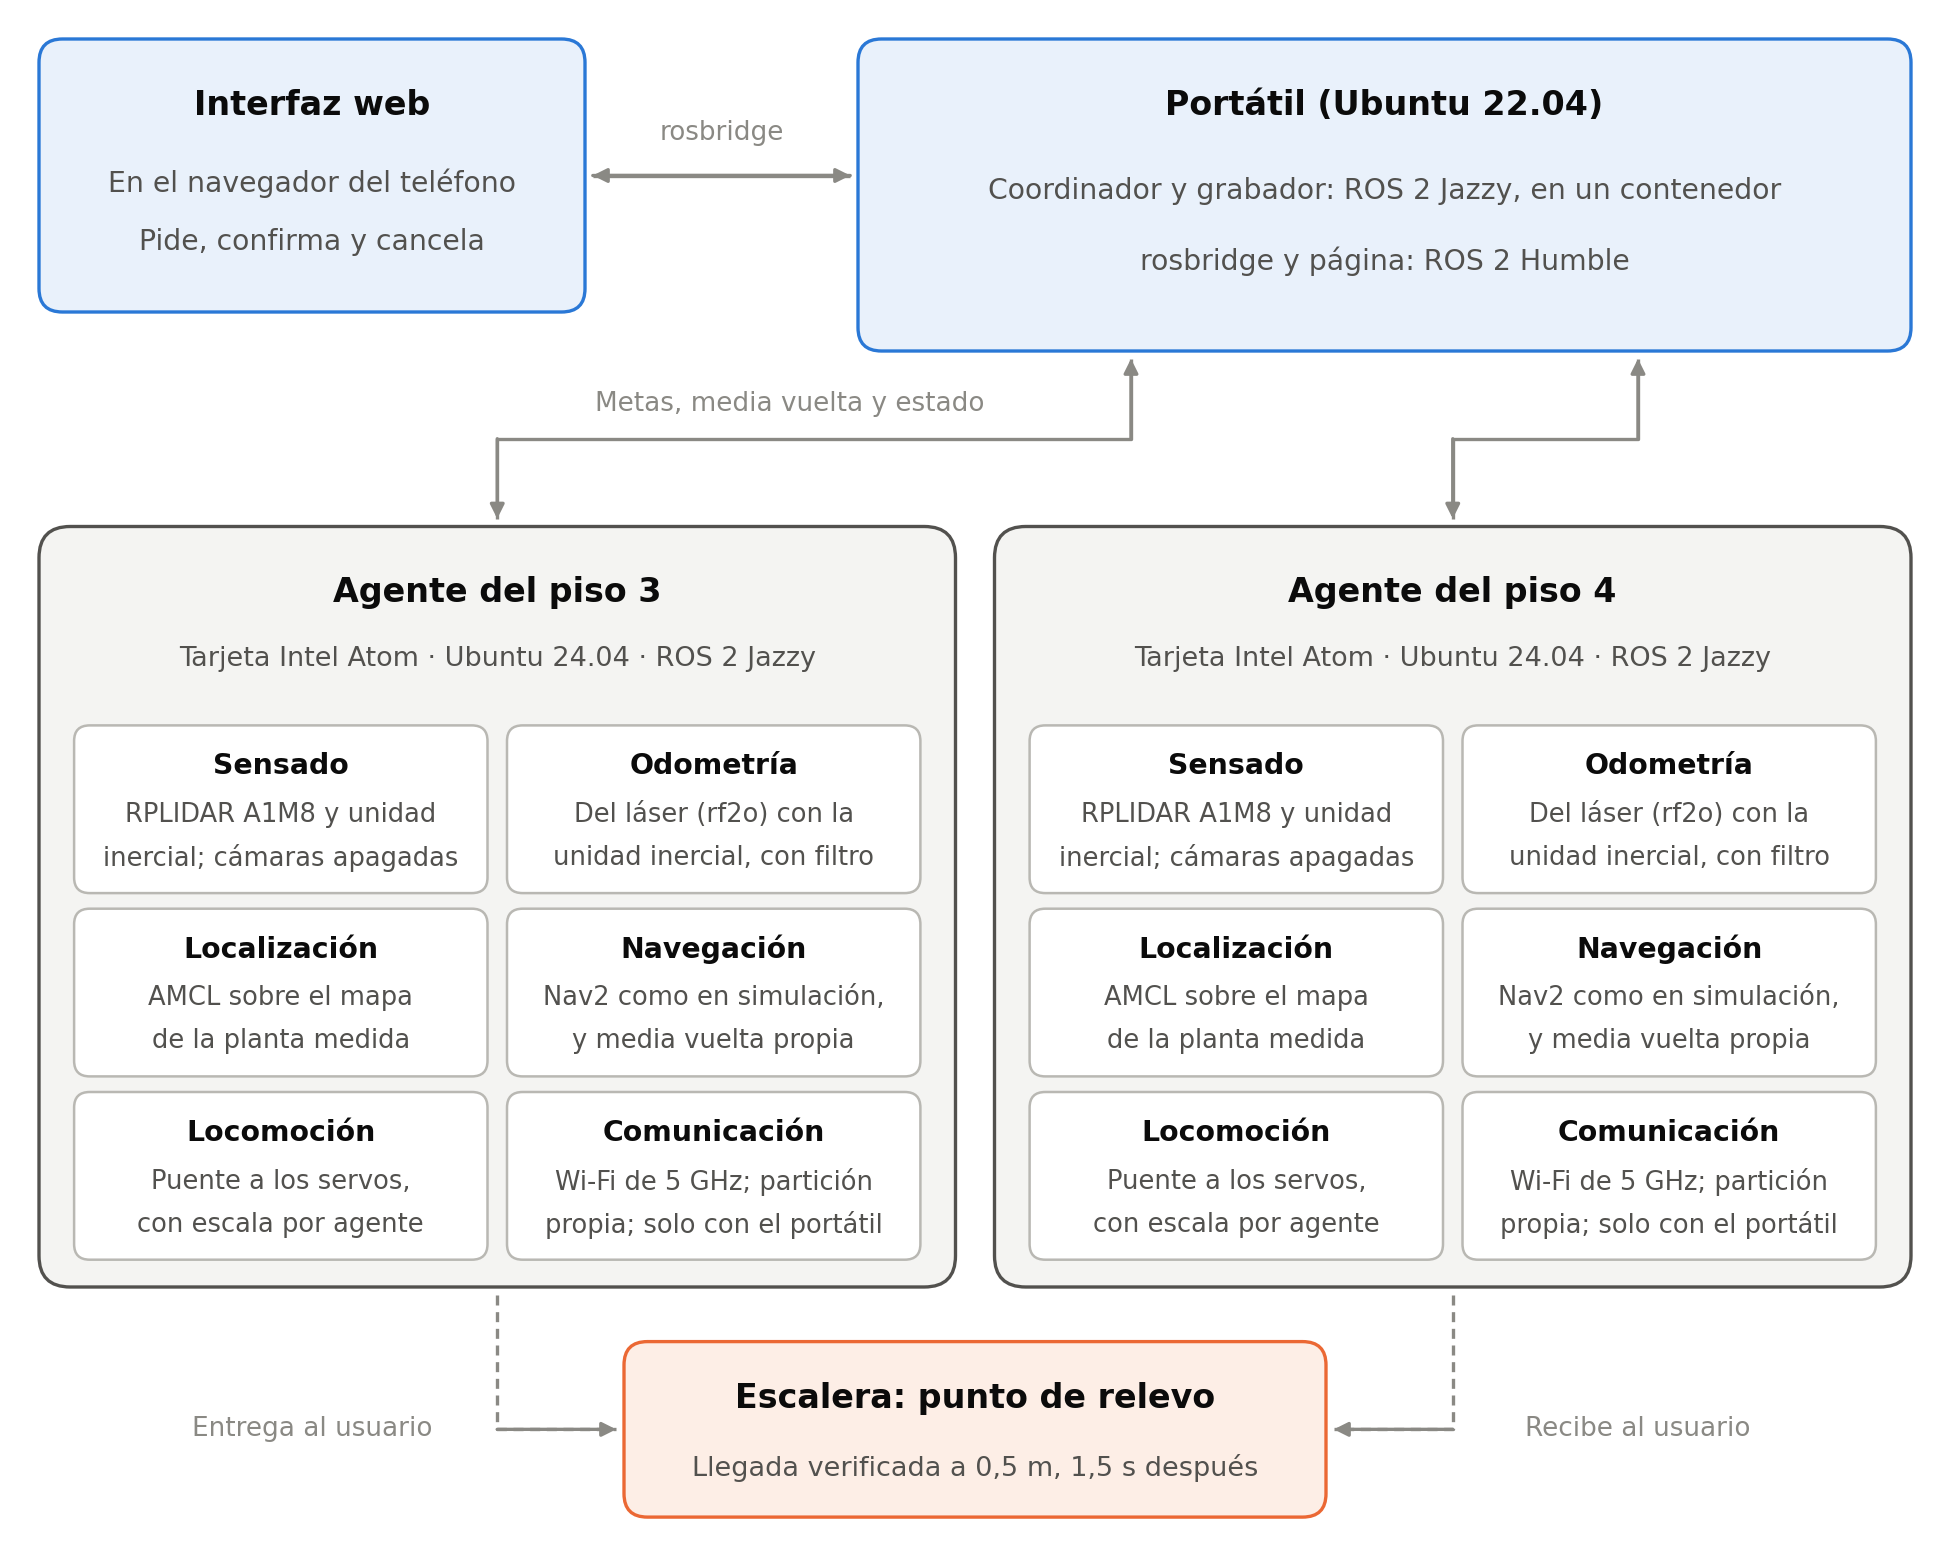
\includegraphics[width=0.86\textwidth]{imagenes/arquitectura_vehiculos.png}
  \caption{Arquitectura del sistema en la campaña con los agentes físicos, en los
    pisos 3 y 4. La estructura es la de la figura~\ref{fig:arquitectura}; cambia
    la implementación de los bloques.}
  \label{fig:arquitectura-vehiculos}
\end{figure}

% =====================================================================
\section{Plataforma robótica}
\label{sec:plataforma}

\subsection{Componentes del agente}
\label{sec:componentes}

Los dos agentes operan con su tarjeta original, para la que el software de la comunidad solo se publica sobre Ubuntu 24.04 con ROS~2 Jazzy, y cada uno atiende un piso
del edificio Catalayud, uno el 3 y otro el 4 (figura~\ref{fig:agentes-fisicos} y tabla~\ref{tab:vehiculo}). El láser que traía el kit no era el que describía el primer informe de hardware, y se identificó
leyendo el modelo que informa el propio sensor.

La autonomía de las baterías limitó la duración de las sesiones de campo. El 29 de septiembre, la batería de tracción de un agente estaba descargada y la de cómputo del
otro se agotó durante la sesión, y esta última volvió a agotarse el 2 de octubre. El 16 de octubre, el portátil se apagó dos veces por falta de batería.

\begin{figure}[htbp]
  \centering
  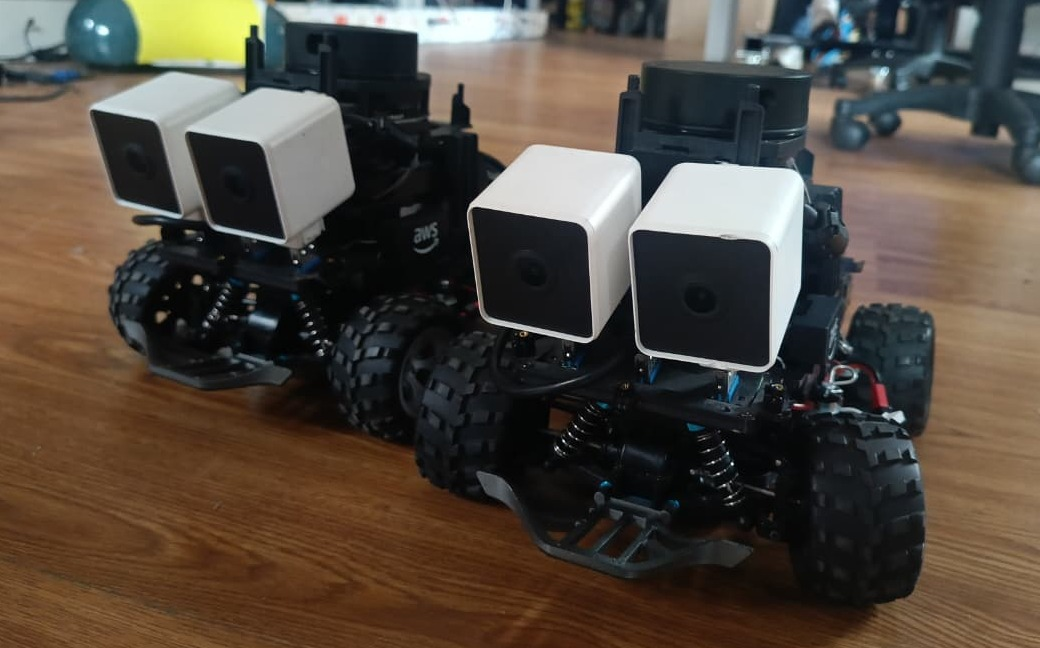
\includegraphics[width=0.62\textwidth]{imagenes/agentes_fisicos.jpg}
  \caption{Los dos agentes físicos, construidos sobre la plataforma AWS DeepRacer, con las dos cámaras al frente y el láser en la parte superior.}
  \label{fig:agentes-fisicos}
\end{figure}

\begin{table}[htbp]
  \centering\small
  \caption{Componentes de cada agente y del portátil.}
  \label{tab:vehiculo}
  \begin{tabular}{@{}p{0.25\textwidth}p{0.68\textwidth}@{}}
    \toprule
    \textbf{Componente} & \textbf{Descripción} \\ \midrule
    Chasis & AWS DeepRacer, escala 1:18, dirección Ackermann, motor de tracción con variador y servomotor de dirección \\ \addlinespace
    Cómputo & Tarjeta original, procesador Intel Atom E3930 de dos núcleos, 4~GB de memoria; Ubuntu 24.04 y ROS~2 Jazzy \\ \addlinespace
    Láser & RPLIDAR A1M8-R5: 360$^\circ$, 360 muestras por barrido, alcance de 0,15 a 12~m, entre 6,8 y 7~Hz \\ \addlinespace
    Unidad inercial & Bosch BMI160 integrada en la tarjeta, por I2C: giroscopio y acelerómetro \\ \addlinespace
    Cámaras & Estéreo; desactivadas por software, porque el sistema no las usa y cargaban la tarjeta \\ \addlinespace
    Alimentación & Una batería para el cómputo y otra de polímero de litio para la tracción \\ \addlinespace
    Portátil & Ubuntu 22.04 y ROS~2 Humble (AMD Ryzen 5 PRO 5650U, 16~GB); el coordinador se ejecuta en un contenedor con Jazzy \\ \bottomrule
  \end{tabular}
\end{table}

\subsection{Nav2 sobre un agente que no gira sobre su eje}
\label{sec:nav2-ackermann}

La configuración por omisión de Nav2 supone tracción diferencial y propone trayectorias que un vehículo tipo automóvil no puede ejecutar. Por ello se sustituyeron dos de
sus tres capas. La planificación global pasó al planificador híbrido A* de Smac con modelo Reeds-Shepp, y el seguimiento, al controlador Regulated Pure Pursuit, los dos con
marcha atrás y con una velocidad deseada de 0,5~m/s. Del árbol de comportamiento se quitó la recuperación que gira sobre el propio eje, con la que el agente, ante un bloqueo,
movía las ruedas sin avanzar hasta agotar los reintentos. Los parámetros tienen una variante por distribución, y una prueba automática falla si se separan en algo distinto de
las diferencias documentadas.

La cadena se puso en marcha con la escalera de siete pasos de la guía oficial de Nav2 \autocite{nav2setup}, cuyo orden va de las transformaciones entre marcos de referencia al
planificador y el controlador, pasando por la odometría, el láser, el mapa, la localización y los mapas de costos. Seguir ese orden permitió aislar el problema de la odometría,
porque una odometría que no mide y un planificador que no planifica se manifiestan igual: el agente no llega. El orden importa también al arrancar, debido a que los mapas de
costos leen el mapa al configurarse, así que el programa de arranque de los agentes activa primero el servidor de mapas y espera a que los seis nodos de la cadena estén
activos. En el laboratorio, la cadena quedó lista en 4~min 4~s en un agente y en 4~min 22~s en el otro.

\subsection{La odometría del láser como limitación principal}
\label{sec:odometria-laser}

Como el agente no tiene codificadores en las ruedas, su única odometría sale de comparar barridos sucesivos del láser. Desde que se midió por primera vez, el 26 de agosto en
simulación, hasta el cambio de edificio, el 2 de octubre, no dio una medida utilizable por falta de información en la señal. En los pasillos del edificio Gregorio registró desde el
1,3~\% del avance real, en simulación, hasta el 73~\%, con un agente físico en el hall del piso 3, y la localización llegaba a separarse más de dos metros de la posición medida con
flexómetro (figura~\ref{fig:hall}).

\begin{figure}[htbp]
  \centering
  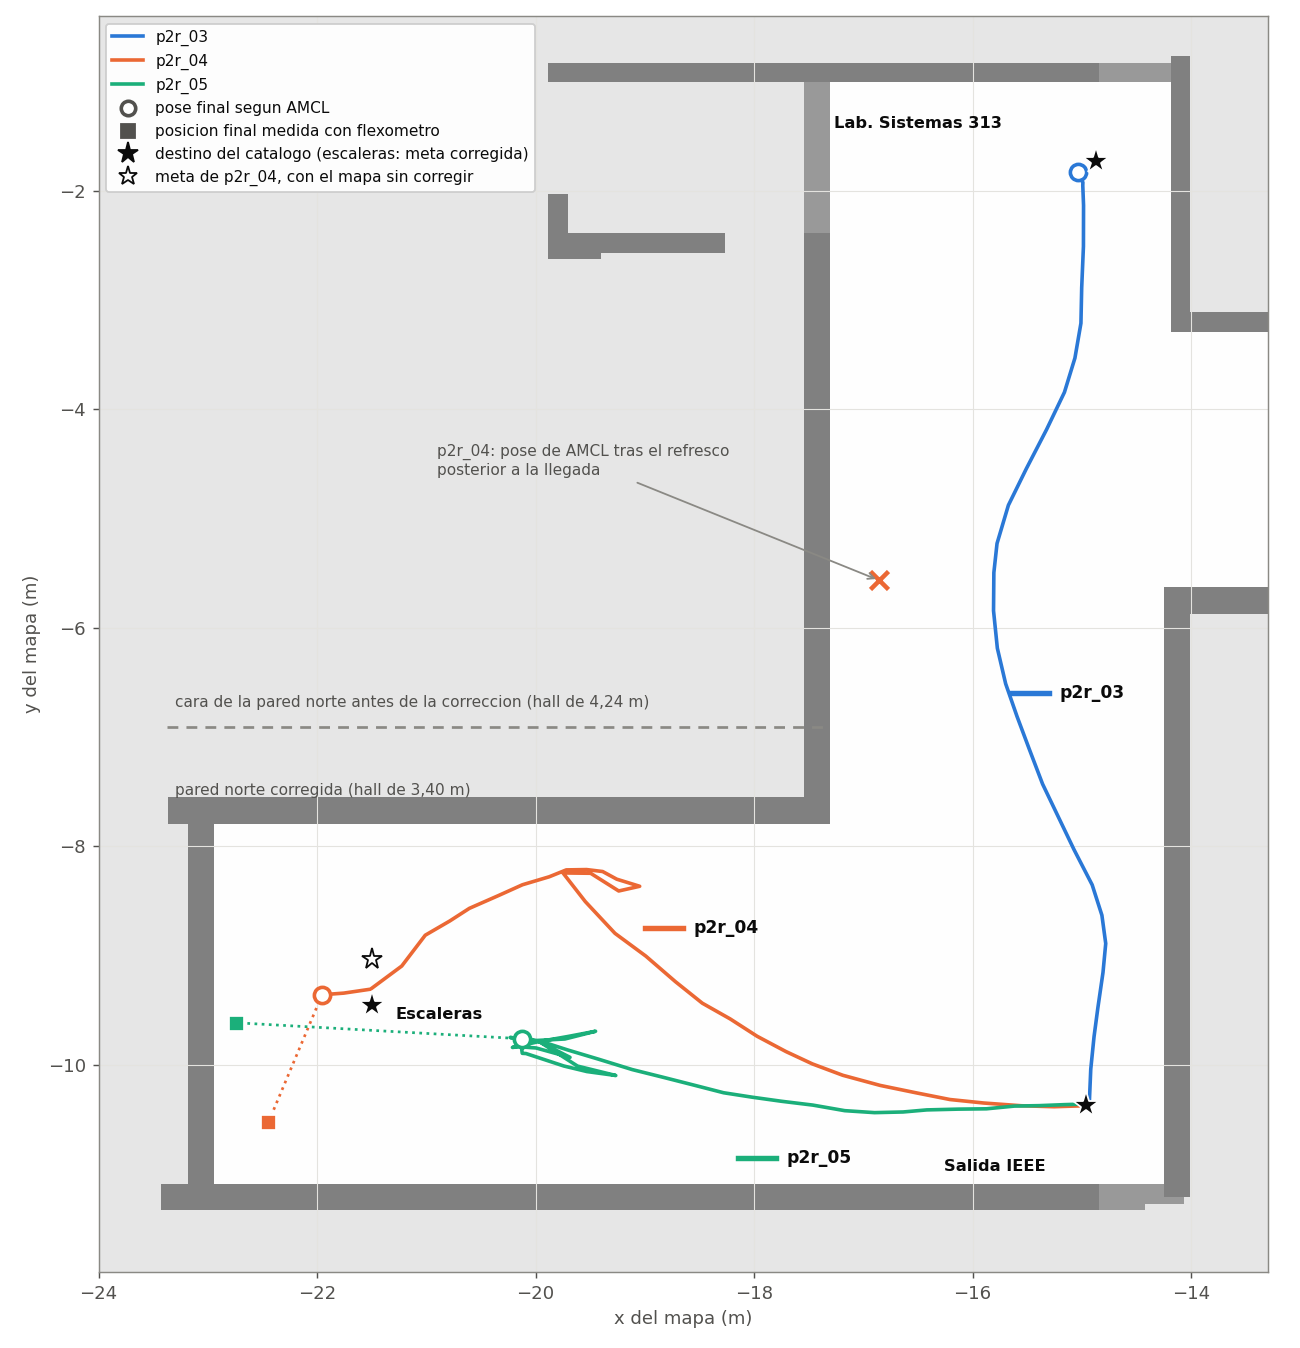
\includegraphics[width=0.6\textwidth]{imagenes/recorridos_hall_piso2.png}
  \caption{Tres recorridos de un agente en el hall del piso 3 del edificio Gregorio. El círculo es la pose que
    da la localización al terminar; el cuadrado, la posición real medida con
    flexómetro. La separación entre los dos es el error, y su causa está en la
    odometría, no en el algoritmo de localización.}
  \label{fig:hall}
\end{figure}

La solución fue cambiar de entorno, con un criterio que salió de la misma medida: hace falta estructura no uniforme dentro del alcance del sensor durante todo el recorrido. Los pisos 3
y 4 del edificio Catalayud la tienen: entre las hornacinas de los salones, los casilleros, la papelera, el ascensor y la escalera suman ocho cambios de perfil en 25~m, uno cada
tres metros. Con la misma odometría y sin cambiar un parámetro, el error cayó por debajo del 5~\% (tabla~\ref{tab:odometria}), lo que hizo posible la demostración física.

\subsection{Los mapas, derivados de medidas con flexómetro}
\label{sec:mapas}

Los intentos de construir el mapa con SLAM en los propios agentes, en septiembre, no dieron un mapa utilizable en ningún pasillo, por la misma falta de información de avance. La vía que
funcionó fue levantar la planta con flexómetro y derivar de ese levantamiento tanto el mundo simulado como el mapa de navegación, de manera que simulación y edificio coinciden al salir de
la misma fuente. En Gregorio esa correspondencia se había dado por supuesta, y al verificarla por primera vez resultó falsa: el modelo daba el hall del piso 3 0,84~m más ancho de lo que
es, 4,24~m frente a 3,40~m, un 25~\% de error. En los pisos 3 y 4 de Catalayud se invirtió el orden: primero se midió y después se modeló.

La herramienta que genera las plantas suma las dos paredes de cada pasillo y avisa si no cierran dentro del 2~\%. Con esa comprobación se encontraron cinco errores antes de generar nada, y
las dos plantas cierran al 0,32~\% y al 0,62~\%. La figura~\ref{fig:mapa4} es el mapa del piso 4, con sus cinco puntos de interés: tres salones, el ascensor y la escalera, que es su punto
de transferencia.

\begin{figure}[htbp]
  \centering
  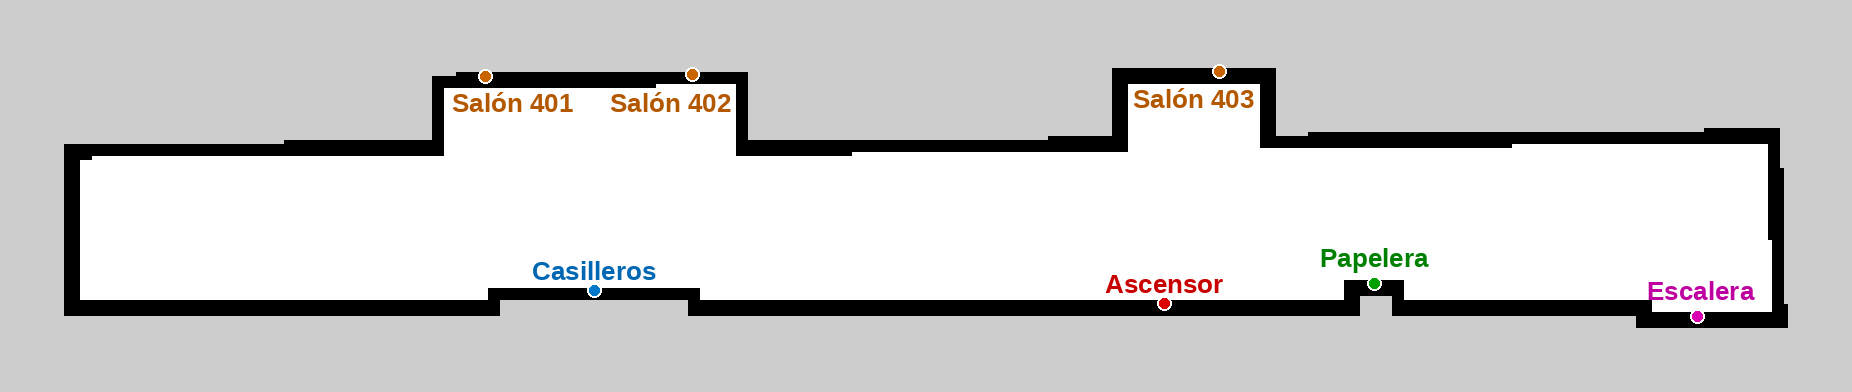
\includegraphics[width=\textwidth]{imagenes/mapa_piso4.png}
  \caption{Mapa de navegación del piso 4, derivado del levantamiento con
    flexómetro. El pasillo se extiende 25~m del extremo norte al sur; los salones
    quedan al este, y el ascensor y la escalera al oeste. Los casilleros y la
    papelera se marcan como referencia del levantamiento.}
  \label{fig:mapa4}
\end{figure}

\subsection{La banda muerta de tracción}
\label{sec:banda-muerta}

Al integrar la cadena de tracción apareció una característica de la plataforma que condiciona la llegada: el agente no se mueve con velocidades pedidas por debajo de 0,40~m/s. El puente que
traduce la orden al variador las convertía en tracción nula, sin ningún aviso, y el agente se detenía al entrar en la fase final del recorrido. Se subió a 0,40~m/s la velocidad
mínima de aproximación del controlador, y después se modificó el puente para que envíe las órdenes menores con el escalón de tracción más bajo.

Como resultado, el agente se aproxima a la meta a 0,40~m/s y no tiene régimen de aproximación fina, un límite de la plataforma que no se corrige afinando el controlador. Además, como la
tracción funciona en lazo abierto, la relación entre la orden y la velocidad real no es igual en los dos agentes, por lo que el puente tiene una escala por agente, ajustada en campo: 0,85
en el del piso 3 y 0,9 en el del piso 4. Con la escala 1,0, el del piso 4 iba a 1,36~m/s y se pasaba de la meta; con 0,9 va a 0,74~m/s.

Ante ese límite, la tolerancia de llegada con los agentes físicos se fijó en 0,5~m antes de las pruebas de navegación, mientras la simulación conserva 0,25~m.

\subsection{La unidad de medición inercial de la tarjeta}
\label{sec:imu}

Al principio el rumbo también salía de la odometría del láser, que en un pasillo recto pierde los giros igual que el avance. Con el agente quieto, ese rumbo derivó hasta 5,9$^\circ$ por minuto,
y un giro de 90$^\circ$ hecho a mano se registró como 19,1$^\circ$. Sin embargo, la tarjeta incluye una unidad de medición inercial, una Bosch BMI160 que el software del fabricante no usa, que,
leída directamente, midió giros de 90$^\circ$ y 360$^\circ$ con un error de 0,1~\% a 1,3~\%, y quieta no se desvió más de 0,3$^\circ$ en 60~s.

Se escribió un nodo que la lee y calibra el sesgo del giroscopio al arrancar. Un filtro de Kalman extendido toma de la odometría del láser el avance y de la unidad inercial el giro; la unidad
publica a 25~Hz y el filtro se ejecuta a 15~Hz, para no cargar la tarjeta. En un giro de 90$^\circ$ contra una línea del piso, el filtro midió 90,17$^\circ$ en un agente y 88,38$^\circ$ en el otro, y
con el agente quieto su rumbo se movió 0,3$^\circ$ o menos por minuto. La posición, en cambio, no mejora, ya que sigue saliendo del láser. Con el rumbo estable se redujo de 1,0 a 0,5~m el margen en
el que Nav2 da la meta por alcanzada, y con ese margen se superó la prueba de navegación de un agente.

\subsection{La red que comunica a los agentes}
\label{sec:dos-vehiculos}
\label{sec:red}

Que dos agentes se repartan un recorrido depende de que puedan comunicarse, así que la red es una condición del relevo.

Como los agentes se mueven, el enlace tiene que ser inalámbrico. La red de la universidad quedó descartada porque aísla a sus clientes entre sí y los agentes no podrían verse; además, no
admite reservas de dirección y no se puede diagnosticar ni modificar. Una red móvil contradiría el diseño, que funciona sin salida a internet porque el edificio no siempre la tiene. Una red
propia sobre Wi-Fi reúne lo que el sistema necesita: control completo, direcciones fijas por dirección física y posibilidad de medir. Su límite conocido es que un enlace compartido no garantiza
tiempos de entrega, por lo que el requisito de red fija cotas numéricas y se verifica midiendo.

\begin{figure}[H]
  \centering
  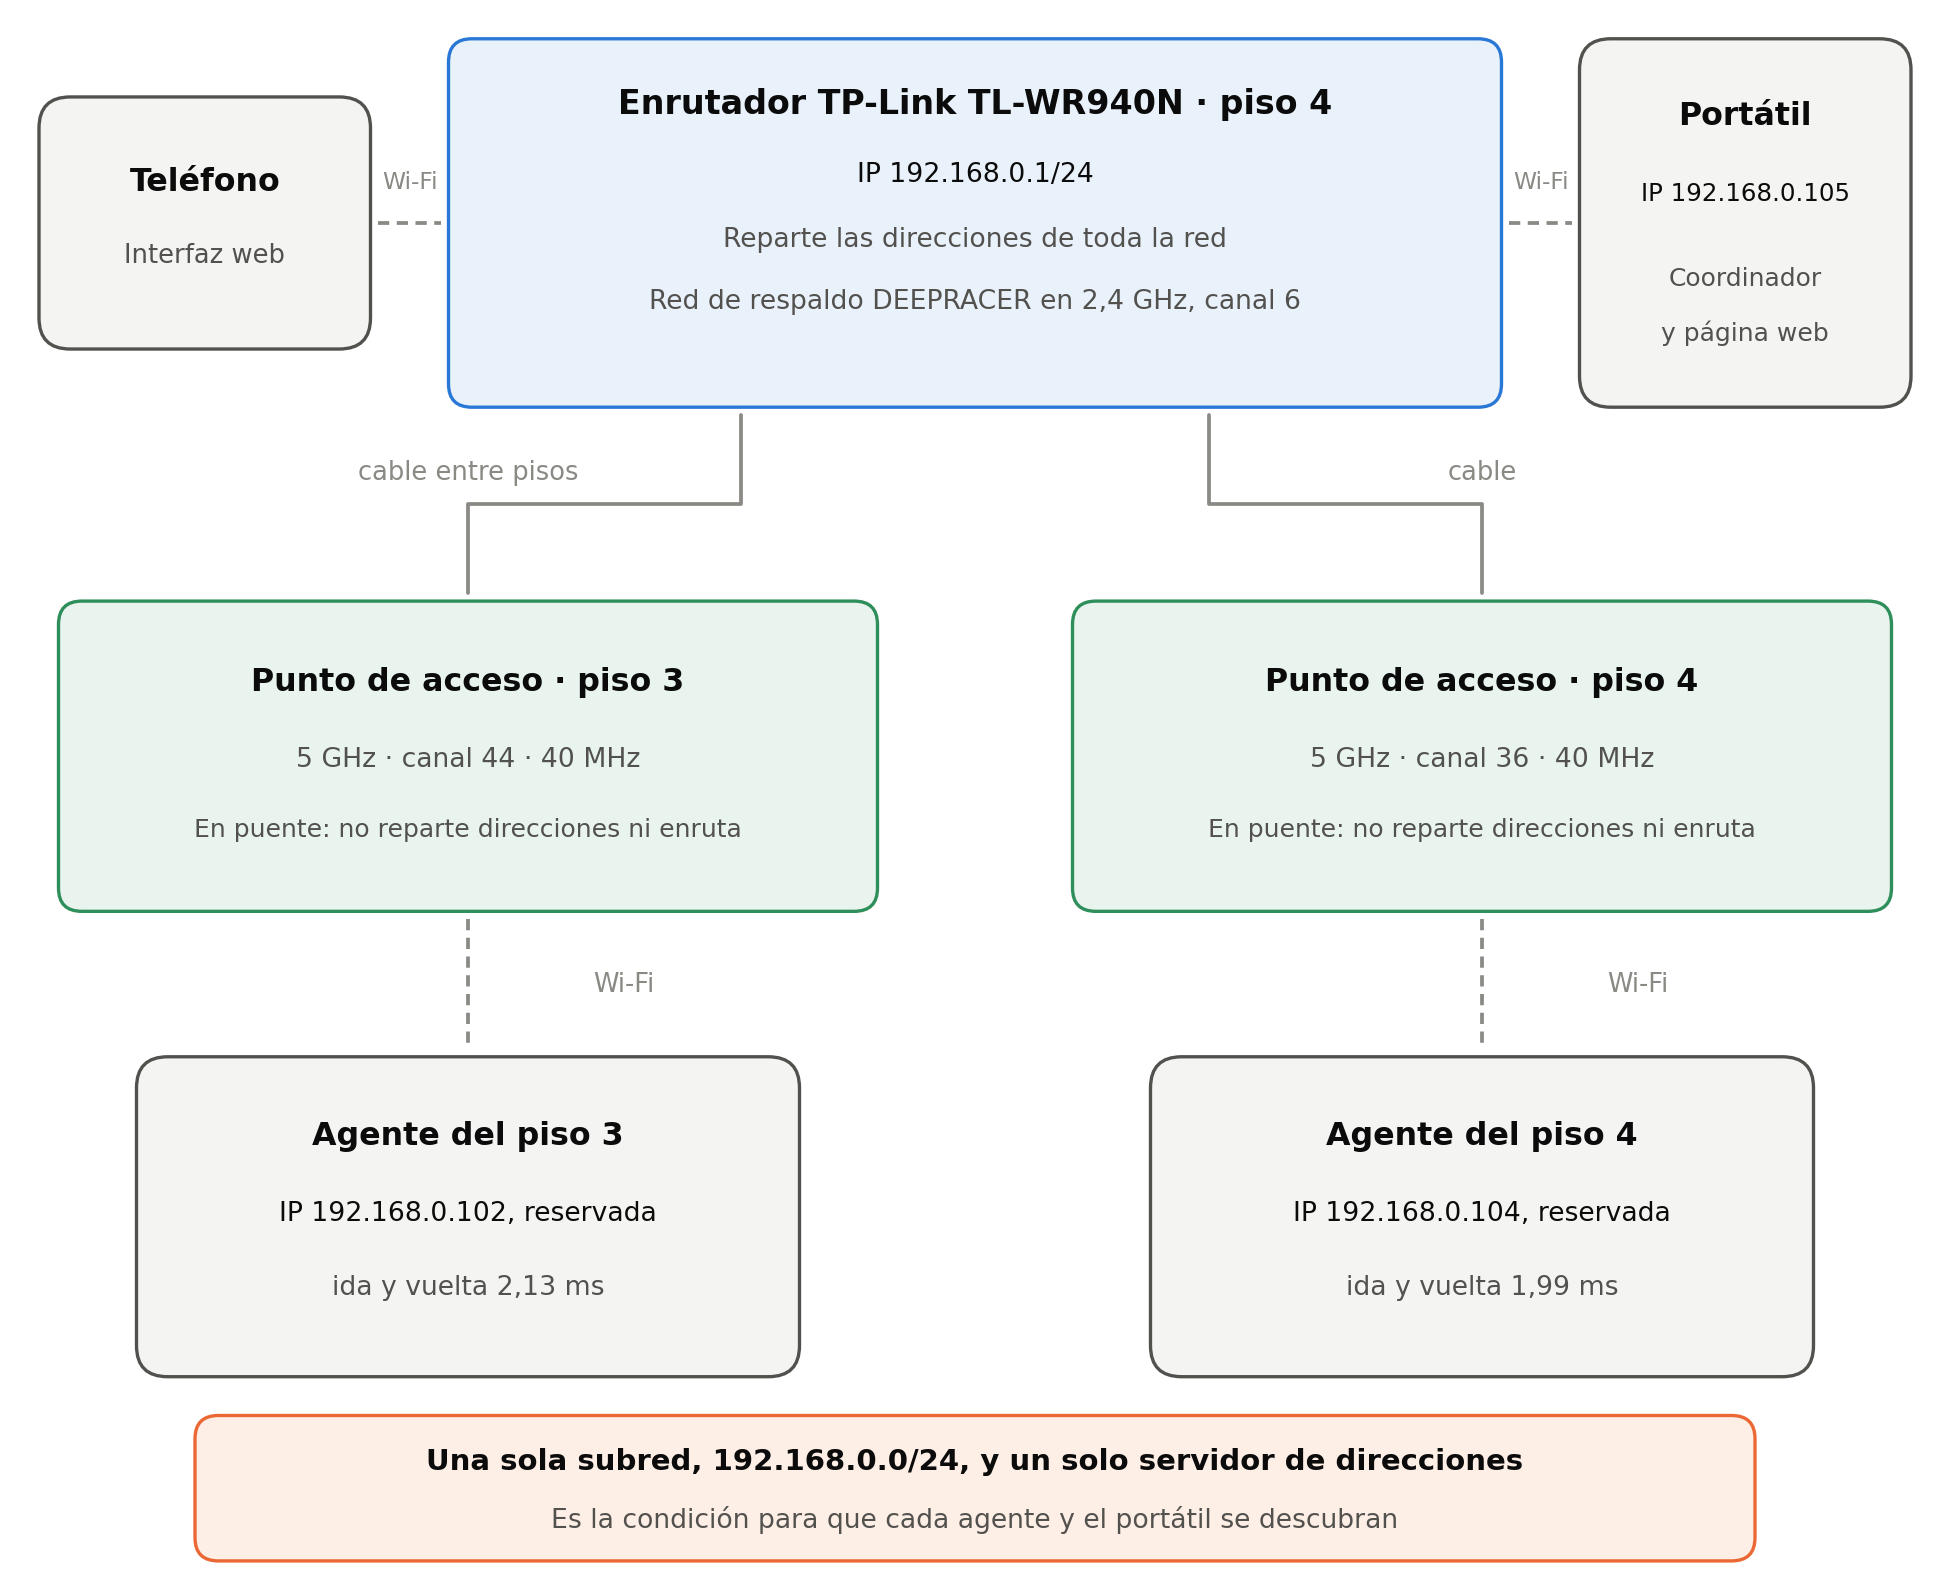
\includegraphics[width=0.96\textwidth]{imagenes/red_topologia.png}
  \caption{Montaje físico de la red. Los dos puntos de acceso trabajan en modo
    puente, de manera que toda la instalación forma una sola subred, la condición
    para que cada agente y el portátil se descubran.}
  \label{fig:red-topologia}
\end{figure}

Un enrutador reparte las direcciones de toda la red, y de él cuelgan por cable dos puntos de acceso, uno por piso. El enrutador une redes, reparte direcciones y encamina entre ellas, mientras que un
punto de acceso solo da acceso inalámbrico a una red que ya existe. Tampoco son repetidores, que enlazan por radio con el resto de la red y usan la misma antena para eso y para sus clientes, con lo que
pierden la mitad del caudal y añaden un salto a cada mensaje; por esa razón, el enlace entre pisos va por cable. Se trabaja en la banda de 5~GHz porque un barrido del sitio encontró 33 redes ajenas en
la de 2,4~GHz y la parte baja de la de 5~GHz prácticamente vacía, y el cambio de banda redujo el percentil 95 del tiempo de ida y vuelta de 20,76 a 11,12~ms. Hay un punto de acceso por piso, en canales
que no se solapan, debido a que la losa atenúa la señal.

Durante la construcción aparecieron defectos que no producían ningún mensaje de error y que solo se encontraron al medir. A las dos tarjetas les faltaba el fichero con las reglas de uso del espectro, por lo
cual veían las redes de 5~GHz pero no podían transmitir en ellas. Un punto de acceso conectado a la vez por cable y por radio ofrecía dos caminos a los mismos mensajes: de 100 peticiones enviadas, un
agente recibía 147, mientras la herramienta de diagnóstico informaba cero por ciento de pérdida. Además, durante una sesión hubo dos servidores de direcciones repartiendo subredes distintas, con lo que
los agentes dejaron de verse al azar.

El problema de mayor efecto estuvo en cuántos procesos se anunciaban por el enlace. En ROS~2 cada proceso se anuncia periódicamente a todos los demás y mantiene el estado de cada uno, con lo que ese
trabajo crece aproximadamente con el cuadrado del número de participantes. Con un agente había del orden de veinte y su tarjeta trabajaba entre el 52 y el 63~\% de capacidad, mientras que al encender el
segundo pasaron a ser del orden de cuarenta y la tarjeta subió al 95~\%, con Nav2 sin alcanzar a arrancar. El tráfico, del orden de 2000 paquetes por segundo, era una fracción despreciable del enlace, y la
navegación gastaba menos: el aumento estaba en los procesos que atienden la red, y el límite fue el costo de procesamiento del descubrimiento.

Restringir el descubrimiento al interior de cada tarjeta bajó el tráfico, pero dejó al coordinador sin ver la navegación de un agente, debido a que el middleware, con pares conocidos, solo anuncia los
primeros participantes de cada máquina. La solución fue cambiar dónde vive el coordinador en vez de cómo se anuncian los procesos: el coordinador y el grabador pasaron al portátil, y cada agente lo tiene como
único interlocutor conocido. Los agentes no se ven entre sí, lo que coincide con el diseño, en el que nunca se comunican directamente. Con ese esquema, el sistema completo volvió a entre el 68 y el 74~\% de la
tarjeta.

Las cotas del requisito, una mediana de 100~ms y un percentil 95 de 250~ms sin pérdidas, se fijaron antes de medir, a partir de los 2~Hz a los que cada agente publica su estado. Entre los dos agentes, en la
misma sala y sobre 600 mensajes, la mediana fue de 5,99~ms y el percentil 95 de 11,12~ms, sin pérdidas, más de un orden de magnitud por debajo de las cotas. Con paquetes de red, entre los dos agentes en el
mismo piso y con dos puntos de acceso, la ida y vuelta fue de 3,75~ms en promedio. En el montaje definitivo, con cada agente en el punto de acceso de su piso, fue de 2,13 y 1,99~ms contra el enrutador, sin
pérdidas ni duplicados. Por lo tanto, la red no limita el desempeño del sistema, cuyos límites están en la plataforma.

\subsection{La media vuelta en varios tiempos}
\label{sec:media-vuelta}

Como en la operación real, cada misión empieza donde terminó la anterior, y el siguiente usuario queda a menudo detrás del agente, que en pasillos de 2,5 a 3,2~m de ancho tiene que dar la vuelta en varios
tiempos. En el piso 4, a la salida del pasillo de 2,5~m, la media vuelta de Nav2 abortó dos veces contra la pared, debido a que el planificador proponía cada segundo una maniobra distinta. Además, con la misma
orden, el motor retrocedía a 1,7 veces la velocidad de avance, por lo que se añadió al puente una escala de 0,75 para la marcha atrás.

La media vuelta se escribió como una maniobra propia del agente, en lugar de seguir ajustando Nav2, que en ese caso trabajaba en el límite de lo que su controlador resuelve. La maniobra alterna marcha atrás y
avance con la dirección a tope y empieza hacia el costado con más espacio. Cada tiempo se corta cuando la huella prevista del agente queda a menos de 0,10~m de un obstáculo, visto por el láser o marcado en el
mapa, donde la escalera está cerrada porque el láser no ve su borde.

El coordinador la pide antes de una meta que queda a más de 110$^\circ$ del rumbo del agente y a más de 1,5~m, y si no se completa en 120~s, sigue Nav2. En sus primeras pruebas giró 160$^\circ$ y 167$^\circ$,
en un solo tiempo cada vez, y en la campaña con los agentes físicos se ejecutó 24 veces.

% =====================================================================
\section{Interfaz de interacción con el usuario}
\label{sec:oe3}

\subsection{La interfaz como página web}

El objetivo pide «una interfaz móvil», y se construyó una página web que se abre en el navegador del teléfono, porque un usuario ocasional no va a instalar nada para preguntar por un salón. La página funciona sin
salida a internet, puesto que la red del edificio puede no tenerla, y no usa bibliotecas ni recursos externos: son un archivo HTML, una hoja de estilo y dos programas en JavaScript, que sirve el propio portátil.
Se comunica con ROS~2 por el puente \textit{rosbridge}, que no tiene autenticación, así que el firewall del portátil solo admite conexiones desde la red de los agentes.

El primer programa es un cliente propio del protocolo del puente, y el segundo es la lógica de la página, que recibe el catálogo de puntos al conectarse y el estado de la misión una vez por segundo, pide y cancela
con la acción de guiado y publica la confirmación de cambio de piso.

\subsection{Lo que el usuario ve}

El usuario elige el origen en una lista y el destino en un catálogo con búsqueda por nombre, donde cada destino muestra su piso y, si queda en el otro piso, la marca «con relevo» (figura~\ref{fig:hri}, izquierda).
Durante la misión, la página muestra un título calculado a partir de la etapa, el texto que redacta el coordinador, el agente que está guiando, hacia dónde va, el destino final y la distancia restante, y una franja de
cinco pasos (preparando, tramo 1, relevo, tramo 2 y fin) marca el paso actual (figura~\ref{fig:hri}, centro).

\begin{figure}[!htbp]
  \centering
  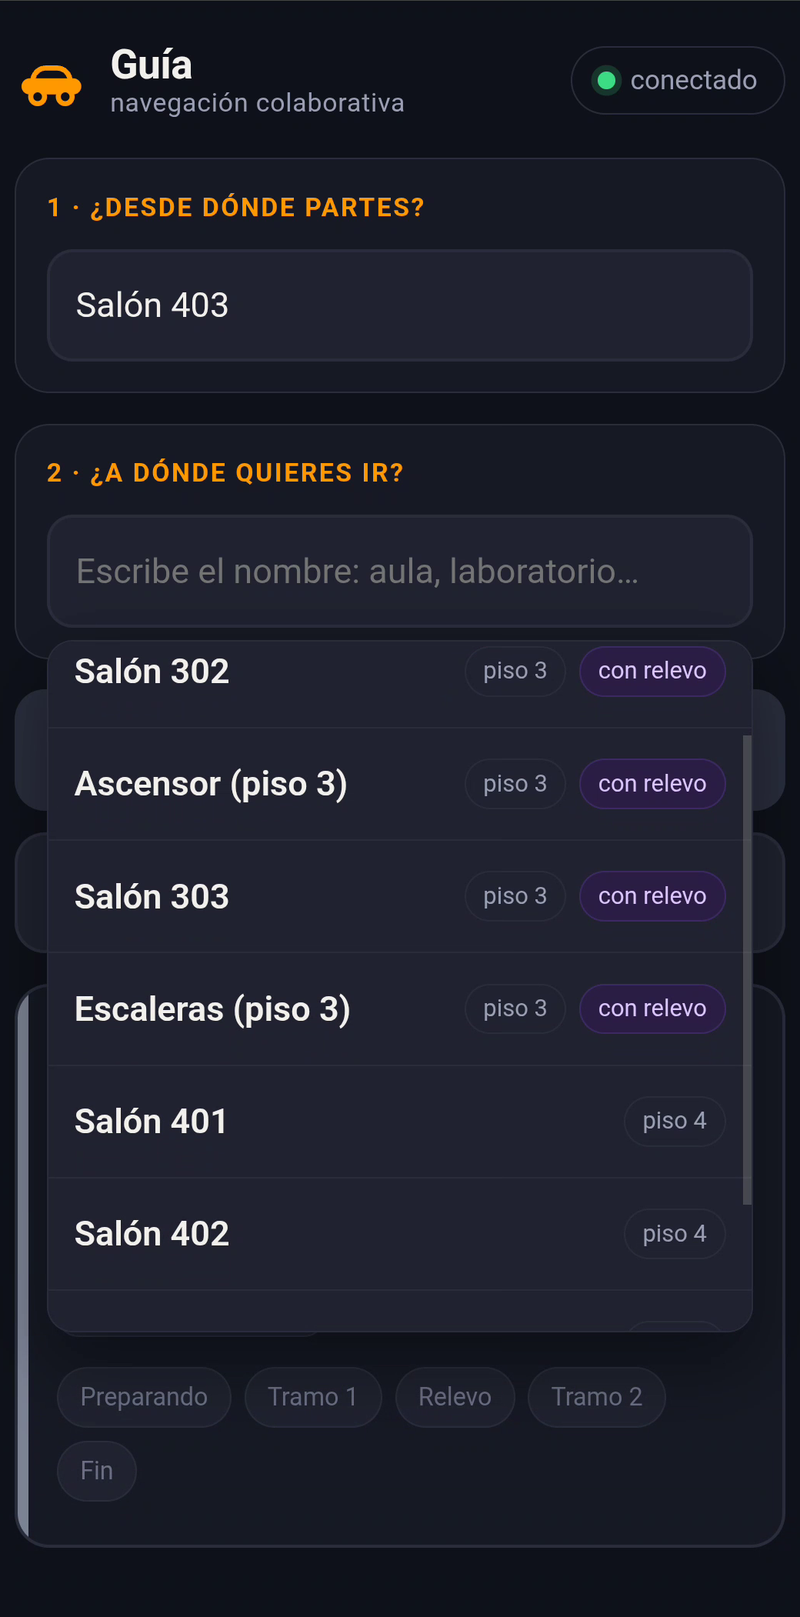
\includegraphics[height=9.2cm]{imagenes/hri_catalogo.png}\hfill
  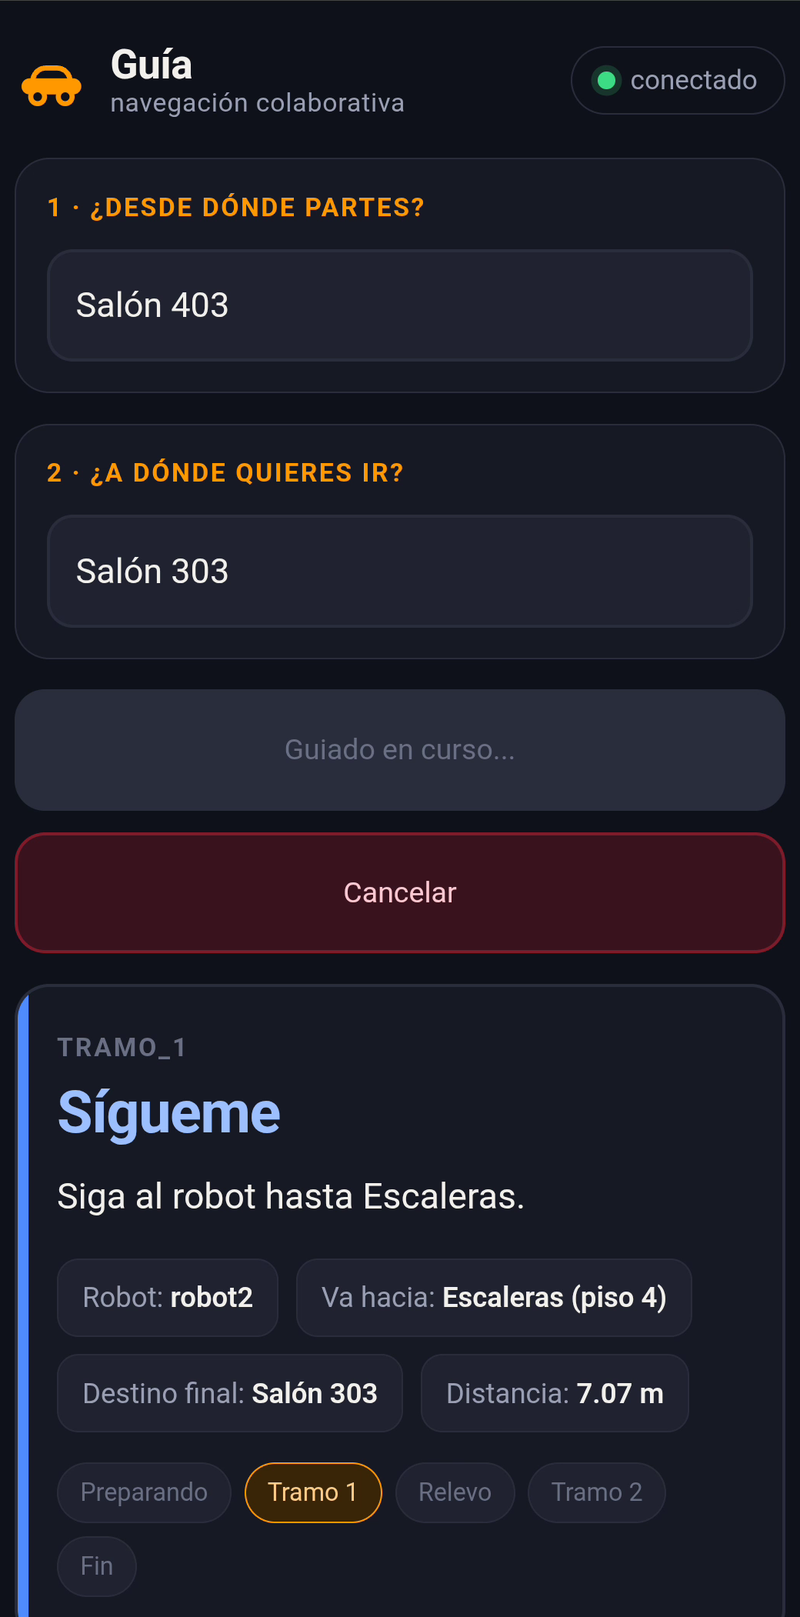
\includegraphics[height=9.2cm]{imagenes/hri_seguimiento.png}\hfill
  \begin{minipage}[b]{4.05cm}
    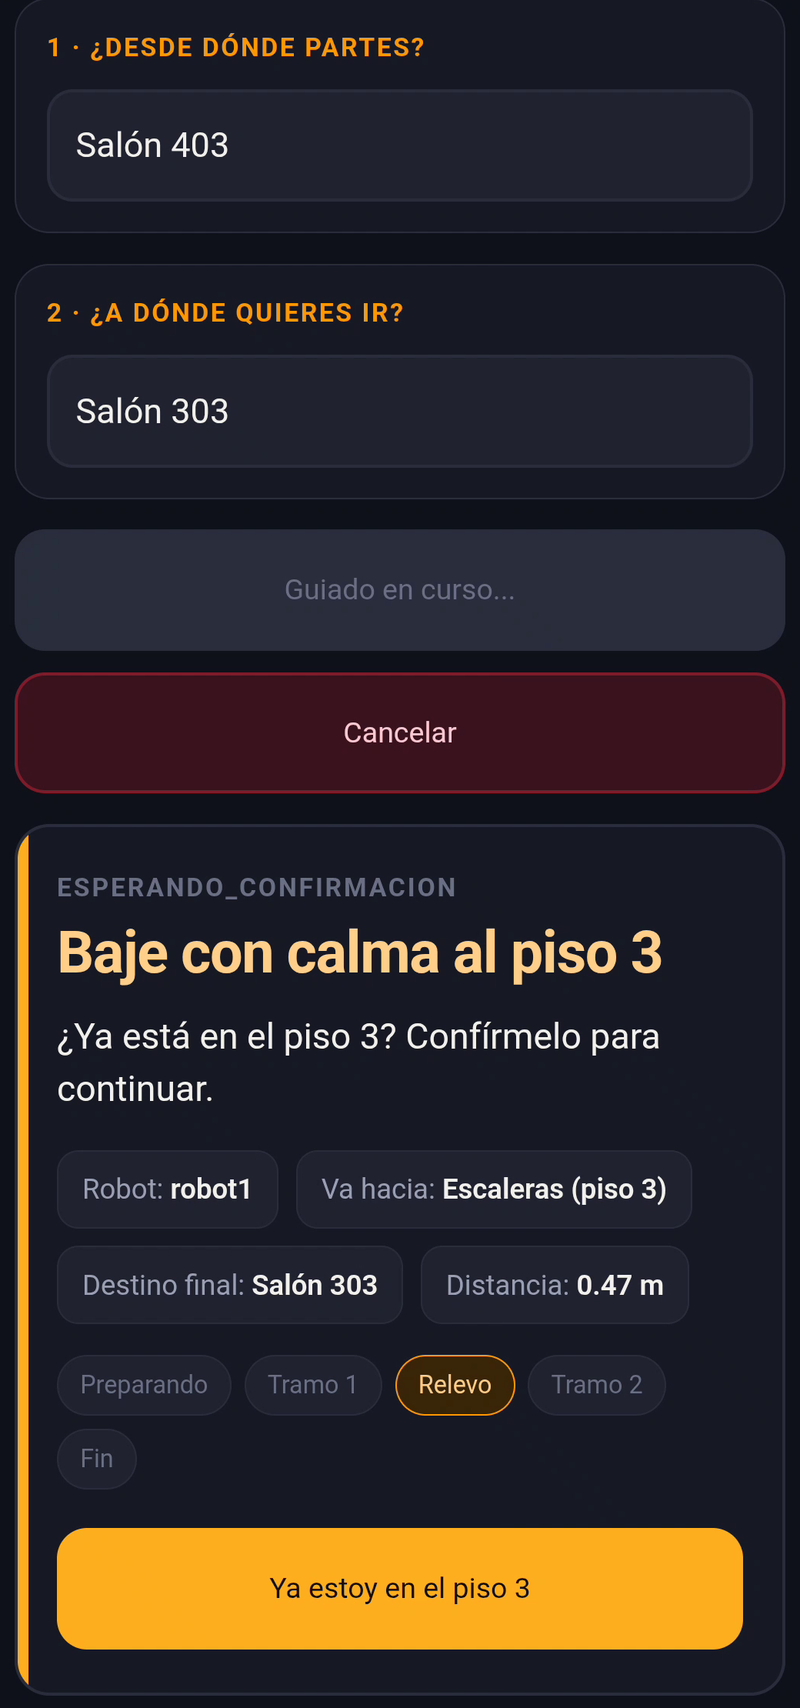
\includegraphics[trim=0 0 0 818,clip,width=\linewidth]{imagenes/hri_confirmacion_piso.png}\\[0.2cm]
    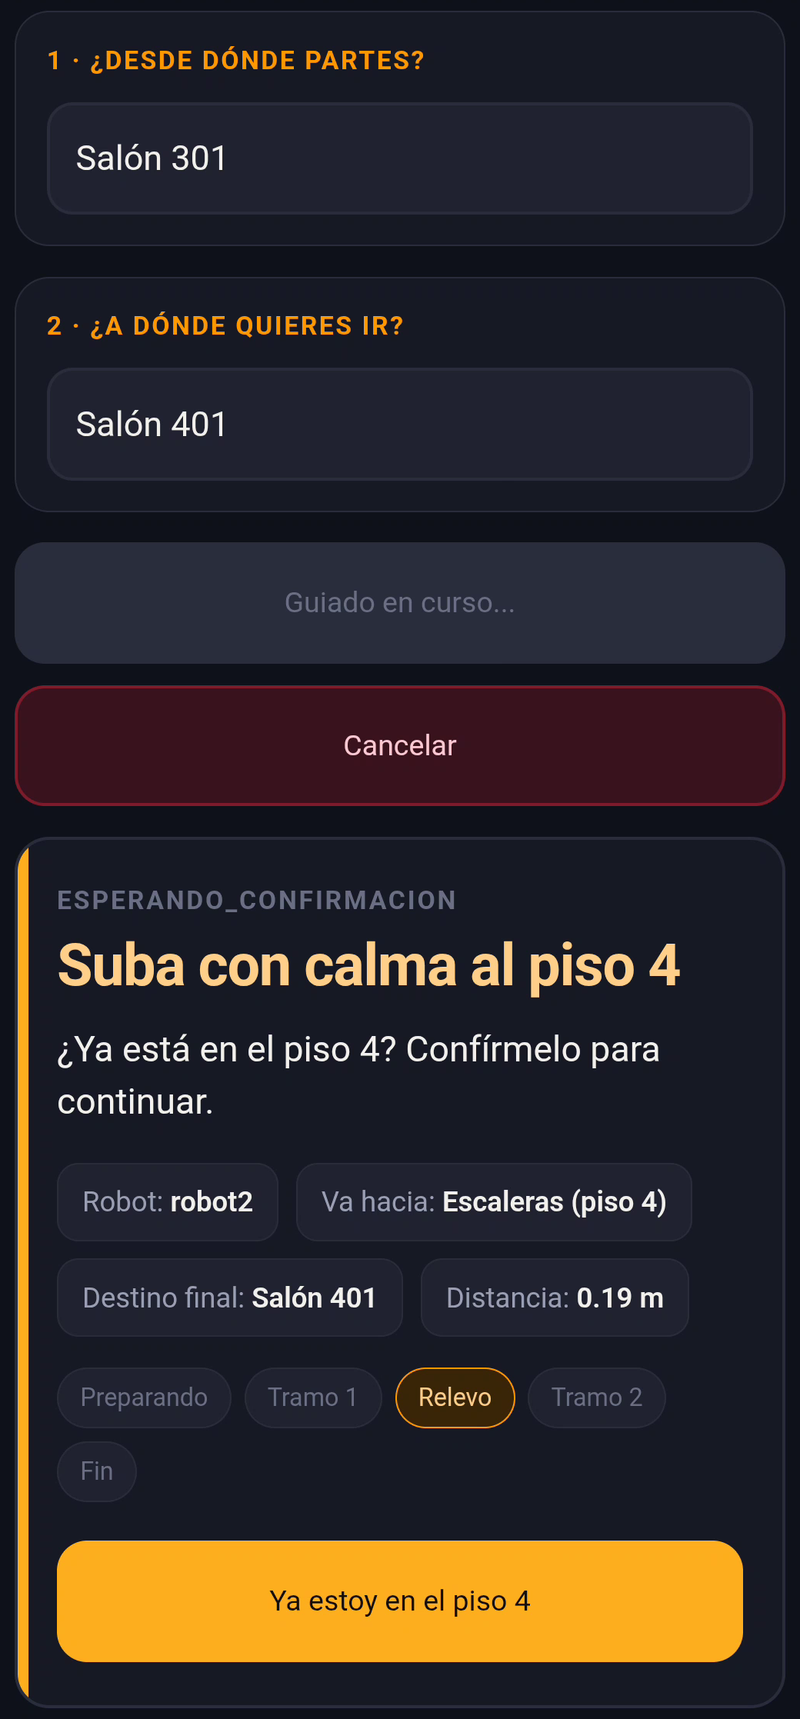
\includegraphics[trim=0 0 0 832,clip,width=\linewidth]{imagenes/hri_confirmacion_subida.png}
  \end{minipage}
  \caption{Interfaz web en el teléfono, en las pruebas del 23 de octubre (anexo A, video 8). A la izquierda, el catálogo de destinos, con el piso de cada uno y la marca «con relevo». En el centro, el primer tramo de una misión, con el texto del coordinador, el agente activo y la distancia restante. A la derecha, la espera de confirmación al bajar y al subir: el título y el botón dicen el sentido y el piso.}
  \label{fig:hri}
\end{figure}

La interfaz se verificó contra el coordinador real: el catálogo, una misión con sus etapas, el texto del coordinador mostrado literal y el botón que se reactiva al terminar. También se operó una misión completa con
relevo desde un teléfono real conectado a la red de los agentes, sin tocar el computador.

\subsection{Confirmación de cambio de piso}

En una misión entre pisos, el segundo agente llega a su escalera y espera al usuario, pero no puede saber si ya subió. Sin una pausa explícita, la misión podía darse por completada con el usuario todavía en el piso
equivocado, y la instrumentación lo habría registrado como éxito. Por esa razón, cuando el segundo agente llega a su punto de transferencia, el coordinador pasa a la etapa de espera de confirmación y la página muestra un
botón para confirmar el cambio de piso, que solo existe en esa etapa (figura~\ref{fig:hri}, derecha). A los 60~s sin confirmación aparece un aviso, y a los 120~s la misión termina como fallida. Los plazos se cuentan desde
que llega el agente, para que un agente lento no le consuma tiempo al usuario, y se miden con el reloj del sistema, sin depender del de la simulación. Si el usuario confirma antes de que el agente llegue, la confirmación se
retiene y se aplica al llegar.

Se verificó en simulación con una ejecución por camino: confirmar a los pocos segundos termina la misión con éxito, confirmar pasados los 60~s hace aparecer el aviso en el teléfono, y no confirmar deja la misión fallida a
los 120~s, con el motivo redactado.

\subsection{Cancelación}

El botón de cancelar existía pero no hacía nada, y no se había detectado. El servidor de acción del coordinador no registraba la función que responde a la cancelación, y ROS~2 rechaza por omisión, sin informar, toda
cancelación que no tenga esa función. Al corregirlo se añadió el comportamiento que faltaba: la misión pasa por la etapa de cancelación, el agente activo regresa al punto de transferencia de su piso, y la misión cierra como
fallida con un texto que lo dice. En simulación, con una ejecución cancelada y una de control, el agente quedó a 0,121~m de su punto de regreso.

Con los agentes físicos se cancelaron seis misiones (anexo A, video 8), al menos una en cada etapa, y en las seis el agente volvió a su escalera, a entre 0,07 y 0,34~m de su punto. En esas pruebas apareció un defecto que la simulación no podía mostrar, pues la media vuelta propia se añadió después. Nav2 conserva durante un tiempo las metas terminadas, y mientras tenía una cancelada en su lista, el agente se declaraba en error y rechazaba la
media vuelta, y Nav2 intentaba girar por su cuenta en el pasillo y oscilaba. Se corrigió haciendo que la media vuelta solo espere a que no haya una meta en curso: antes de la corrección se rechazaron ocho de quince
medias vueltas, y después ninguna de diez.

\subsection{Ajustes tras las pruebas con los agentes físicos}
\label{sec:ajustes-campo}

En las pruebas con los agentes físicos aparecieron además defectos de la página. El título de la etapa de confirmación preguntaba siempre «¿Ya subió?», lo que al subir resultaba brusco y al bajar del piso 4 al 3 era falso, por
lo que pasó a salir de comparar el piso de origen con el del agente que espera, como «Suba con calma al piso 4» o «Baje con calma al piso 3» (figura~\ref{fig:hri}), y el botón dice «Ya estoy en el piso 4», o el piso que
corresponda.

Ese cambio se hizo el día de la campaña, antes de ejecutarla, y aun así los teléfonos mostraron la versión anterior, debido a que el servidor no le indicaba al navegador cuándo volver a pedir la página. Desde entonces la
página se sirve con la indicación de comprobarla cada vez que se abre. Por otra parte, los dos ascensores se llamaban igual en la lista y en una misión se eligió el del piso equivocado, así que los nombres repetidos se
muestran con su piso, como «Ascensor (piso 3)» (figura~\ref{fig:hri}, izquierda). Los tres ajustes se verificaron con pruebas automáticas y después con un teléfono y los agentes físicos, en una misión de subida y otra de
bajada.

% =====================================================================
\section{Protocolo experimental e instrumentación}
\label{sec:protocolo}

El protocolo se escribió antes de instrumentar el sistema, porque un protocolo redactado después de ver los datos tiende a acomodarse a lo que salió, por ejemplo eligiendo el umbral que deja fuera las ejecuciones malas. Fija
las métricas con su definición operativa, el criterio de éxito, el tamaño de muestra y una lista cerrada de causas de descarte, y cada versión queda fechada en el historial del repositorio.

\subsection{Definiciones operativas}

Una métrica sin un evento de inicio y uno de fin medibles por una máquina no se puede informar, y por eso la tabla~\ref{tab:metricas} da los dos eventos de cada una. Todas las marcas salen de un mismo reloj: en simulación, el de la
simulación; en los agentes físicos, el del computador que graba.

\begin{table}[htbp]
  \centering\small
  \caption{Definición operativa de las cuatro métricas del anteproyecto.}
  \label{tab:metricas}
  \begin{tabular}{@{}p{0.2\textwidth}p{0.36\textwidth}p{0.36\textwidth}@{}}
    \toprule
    \textbf{Métrica} & \textbf{Inicio} & \textbf{Fin} \\ \midrule
    Tiempo de respuesta & El coordinador acepta la solicitud & Primera de tres muestras seguidas de la odometría del agente asignado con velocidad de al menos 0,02~m/s \\ \addlinespace
    Tiempo de asignación & Primera publicación de la etapa recibida & Primera publicación del primer tramo, con el agente asignado \\ \addlinespace
    Tasa de éxito & \multicolumn{2}{p{0.72\textwidth}}{Proporción de misiones exitosas sobre las ejecuciones válidas} \\ \addlinespace
    Continuidad entre niveles & El primer agente alcanza su punto de transferencia & Primer movimiento del segundo agente \\ \bottomrule
  \end{tabular}
\end{table}

Una misión es exitosa si la pose final del agente, en su odometría, está a 0,25~m o menos del destino declarado en el catálogo (0,5~m en los agentes físicos), si llegó a la etapa completada sin pasar por fallida y, cuando era entre
pisos, si hubo un relevo.

La regla central del protocolo es que el éxito se mide contra la odometría del agente, sin tomar por válido el resultado que devuelve Nav2. Una navegación puede terminar en éxito y haber dejado al agente lejos del destino: en las
primeras pruebas en simulación, una de tres metas devolvió éxito con el agente a 0,296~m. Aceptar ese resultado sería dejar que el sistema se evalúe a sí mismo.

El tiempo de asignación resultó menor que el paso de 100~ms del reloj de la simulación, así que se informa como una cota por misión y se caracterizó aparte, en un banco de pruebas con el reloj del sistema. La continuidad se definió
primero como una condición binaria, que resultó no poder fallar, y se reemplazó por el intervalo del relevo, una magnitud que sí varía.

\subsection{Diseño de la campaña en simulación}

La campaña en simulación tiene treinta misiones en dos grupos de quince. En las de un mismo piso, el origen y el destino coinciden en el piso y no hay relevo y sirven de comparación; en las de dos pisos hay un
relevo, y son las que responden la pregunta de investigación.

Los pares de origen y destino salen de un sorteo, porque con pares elegidos a mano se corre el riesgo de probar justo los recorridos que funcionan. Se sortean entre los puntos del catálogo menos los dos puntos de transferencia, catorce
en el piso 2 y quince en el piso 3, que dan 392 pares posibles dentro de un mismo piso y 420 entre pisos, y ningún par se repite. La semilla del sorteo es la fecha en que se hace, escrita como año, mes y día, y el listado se guarda en
el repositorio antes de la primera ejecución, de manera que nadie puede probar semillas hasta obtener un sorteo conveniente.

Las diez primeras misiones salieron de un sorteo con la semilla 20260822 en el que todas las misiones entre pisos subían del piso 2 al 3 y todas las de un solo piso se quedaban en el 2. El grupo con relevo era el único que navegaba por
el piso 3, y una diferencia entre los grupos no habría podido atribuirse al relevo. Por esa razón, las veinte restantes se sortearon de nuevo el 4 de septiembre, con la semilla 20260904, para que cada grupo quedara repartido
entre los dos pisos: en el de un mismo piso, ocho misiones en el piso 2 y siete en el 3; en el de dos pisos, ocho de subida y siete de bajada.

Una ejecución fallida cuenta como fallo. Solo se descarta si la causa es ajena al sistema y está en una lista cerrada, escrita antes de la campaña, que admite la caída del simulador, un controlador del agente que no se activa, el factor
de tiempo real por debajo de 0,99, un fallo de la máquina anfitriona o una cancelación por una causa externa anotada antes de conocer el resultado. Si los descartes superan el 20~\% de las ejecuciones, la campaña no es válida.

\subsection{Instrumentación}
\label{sec:instrumentacion}

Cada misión deja una grabación de datos de ROS (\textit{rosbag}) con los tópicos del coordinador y de los dos agentes. A partir de ella, un programa compone el registro de la misión, en un formato estructurado que se valida contra un
esquema versionado y que contiene las marcas de cada etapa, la trayectoria de cada agente, la pose final, el error de llegada y su procedencia. Un segundo programa comprueba la integridad de los registros y calcula las cuatro métricas con
sus intervalos de confianza. Este programa se escribió antes de la campaña, y con él se encontraron dos defectos que después habrían sido irreparables: la continuidad no tenía campo en el esquema, y el intervalo que citaba el protocolo no
se reproducía con el método declarado.

Con los agentes físicos, el grabador se ejecuta en el contenedor con Jazzy, y un programa adapta la grabación al formato que leen las herramientas de Humble. El registro usa el reloj del computador, la tolerancia de 0,5~m y el mapa de cada piso.
La llegada la verifica el coordinador con la pose que publica el agente, 1,5~s después de que Nav2 la da por alcanzada (figura~\ref{fig:instrumentacion}), pues Nav2 la declara en cuanto el agente entra en su margen, y el agente sigue
rodando. En las llegadas medidas en el piso 4, el agente estaba a entre 0,53 y 0,62~m de la meta en la última orden de avance, y un segundo después, ya quieto, a entre 0,09 y 0,53~m. La distancia de llegada se guarda con su procedencia,
medida con flexómetro o tomada de la localización del agente, y el programa de análisis advierte cuando no hay medida externa, como ocurrió en la campaña con los agentes físicos.

\begin{figure}[!htbp]
  \centering
  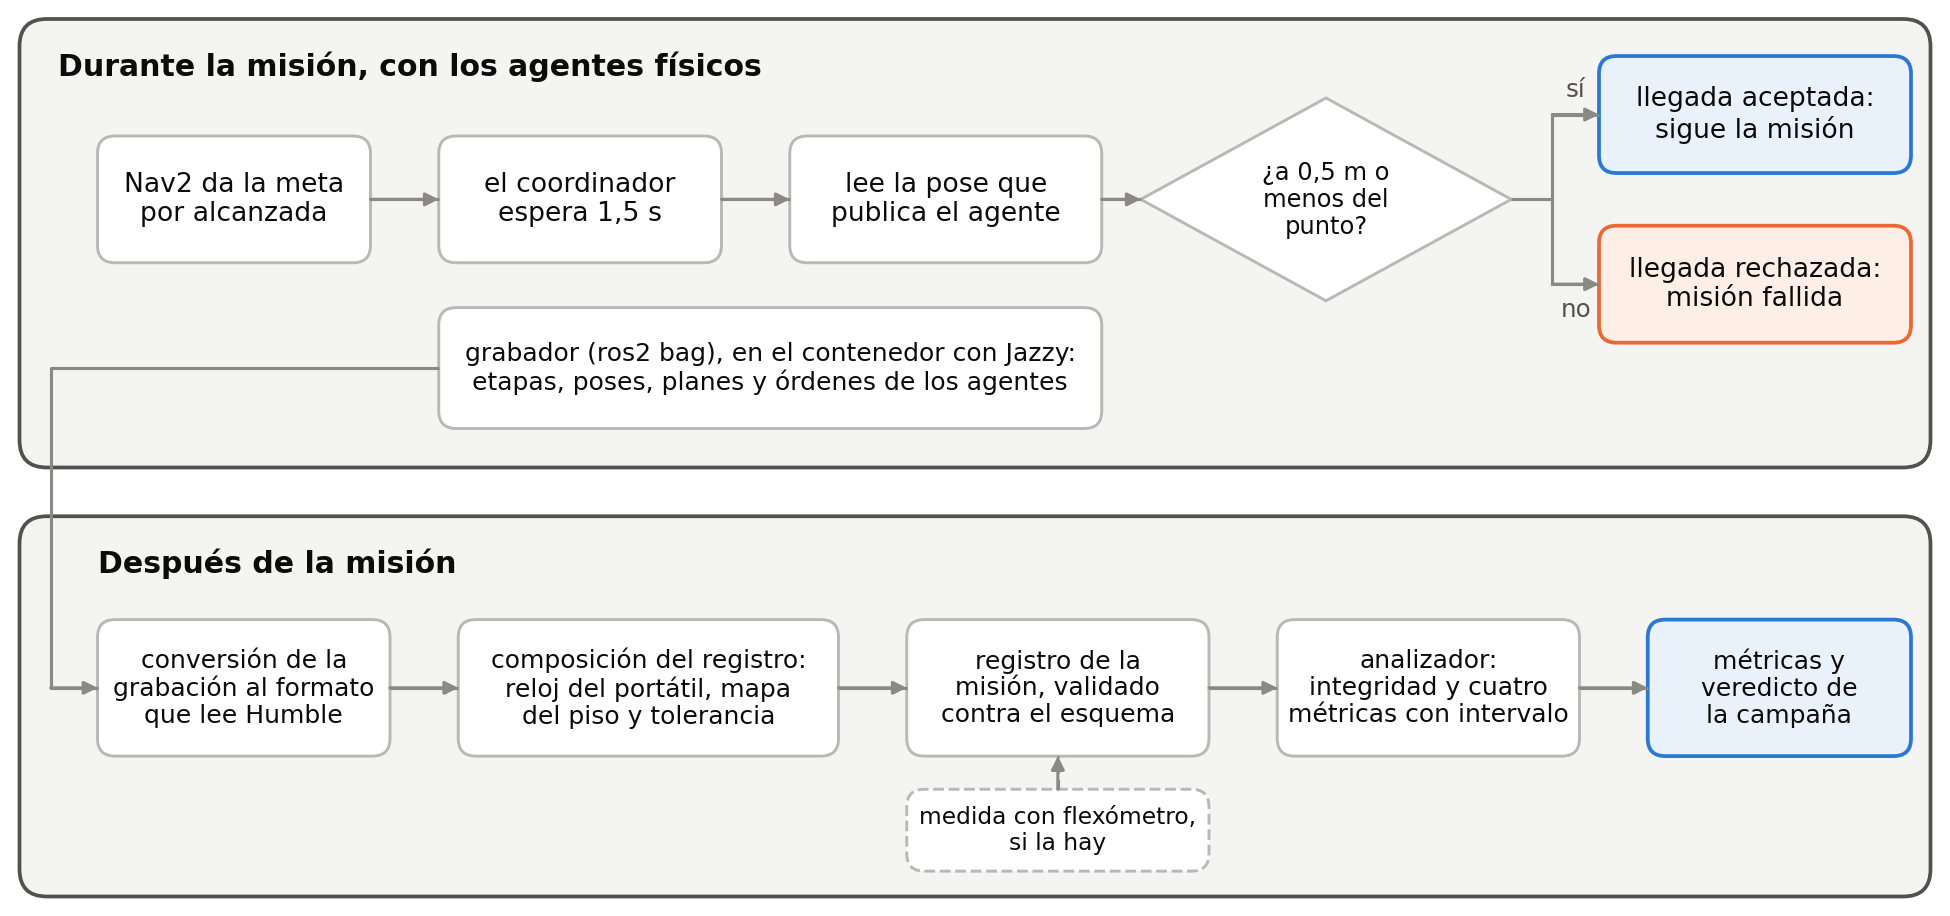
\includegraphics[width=\textwidth]{imagenes/instrumentacion.png}
  \caption{Instrumentación de una misión. Arriba, la verificación de la llegada que hace el coordinador con los agentes físicos; abajo, el camino de la grabación hasta las métricas de la campaña. En simulación el camino es el mismo, sin la conversión de formato y con la tolerancia de 0,25~m.}
  \label{fig:instrumentacion}
\end{figure}

\subsection{Pruebas de verificación de la demostración física}
\label{sec:pruebas-verificacion}

La demostración con los agentes físicos se organizó en seis pruebas de verificación sucesivas, cada una con un criterio escrito antes de ejecutarla y con lo que significa no superarla (tabla~\ref{tab:pruebas-verificacion}). Se fijaron tres
fechas de revisión en octubre, y la toma de datos se cerró con la última, el 16 de octubre.

\begin{table}[htbp]
  \centering\small
  \caption{Pruebas de verificación de la demostración física y su estado al
    cerrar la toma de datos.}
  \label{tab:pruebas-verificacion}
  \begin{tabular}{@{}p{0.24\textwidth}p{0.52\textwidth}p{0.16\textwidth}@{}}
    \toprule
    \textbf{Prueba} & \textbf{Criterio} & \textbf{Estado} \\ \midrule
    Actuación & El agente responde a las órdenes de dirección y tracción & Superada \\ \addlinespace
    Odometría & Error de 10~\% o menos sobre un recorrido conocido de 5~m o más & Superada \\ \addlinespace
    Navegación de un agente & Un agente llega de un punto a otro con Nav2, con la llegada verificada & Superada \\ \addlinespace
    Dos agentes en la misma red & Los dos agentes y el coordinador coexisten sin conflicto de nombres & Superada \\ \addlinespace
    Misión con relevo & Una misión con relevo sobre los dos agentes, con su registro & Superada \\ \addlinespace
    Campaña con los agentes físicos & Entre 5 y 10 repeticiones del protocolo con su registro & Superada \\ \bottomrule
  \end{tabular}
\end{table}

Para la campaña con los agentes físicos se sortearon el 13 de octubre, con la semilla 20261013, diez misiones entre los pisos 3 y 4 del edificio Catalayud: cinco de subida y cinco de bajada. Se ejecutaron en ese orden y sin reubicar los agentes entre misiones, como ocurriría en la operación real.

% =====================================================================
%  RESULTADOS (versión de revisión)
%  Correcciones del 4 de noviembre: ideas enlazadas, menos repeticiones y la secuencia
%  de la detención de la navegación con el apagado del portátil. Ninguna cifra de
%  resultado sale del capítulo.
% =====================================================================
\chapter{Resultados}
\label{cap:resultados}

Las dos campañas se presentan por separado porque responden a preguntas distintas. La de simulación, con treinta misiones, da la evidencia estadística sobre la tasa de éxito. La de los agentes físicos, con diez misiones sorteadas en los pisos 3 y 4 del edificio Catalayud, muestra que el sistema completo se puede llevar a un edificio real, donde intervienen los sensores, la red inalámbrica y la tracción de los agentes, y donde los usuarios piden, siguen y confirman las misiones desde un teléfono. En las dos campañas, todos los fallos ocurrieron en la navegación de un agente, sobre todo en la precisión de su llegada, y ninguno en la asignación ni en el relevo, que son el núcleo del proyecto.

% ---------------------------------------------------------------------
\section{Evaluación en simulación}
\label{sec:res-sim}

En la campaña se ejecutaron treinta misiones sorteadas (anexo A, video 6): quince con origen y destino en el mismo piso, sin relevo, que sirven de comparación, y quince entre pisos, con un relevo. Según el programa de análisis la campaña es válida, sin ningún descarte, frente a un máximo admitido del 20~\%.

\subsection{Tasa de éxito}

Una misión es exitosa si la pose final queda a 0,25~m o menos del destino, medida contra la odometría, sin importar lo que informe Nav2, y si llega a completarse sin pasar por fallo. La tabla~\ref{tab:exito} da la tasa de cada grupo con su intervalo de confianza de Wilson al 95~\% \autocite{wilson1927probable}.

\begin{table}[htbp]
  \caption{Tasa de éxito de la campaña en simulación, con intervalo de confianza
    de Wilson al 95~\%.}
  \label{tab:exito}
  \begin{tabular}{@{}lcccc@{}}
    \toprule
    \textbf{Misiones} & \textbf{n} & \textbf{éxitos} & \textbf{tasa} & \textbf{intervalo al 95~\%} \\ \midrule
    Campaña completa & 30 & 26 & 86,7 \% & 70,3 -- 94,7 \% \\
    Mismo piso, sin relevo & 15 & 12 & 80,0 \% & 54,8 -- 93,0 \% \\
    Entre pisos, con relevo & 15 & 14 & 93,3 \% & 70,2 -- 98,8 \% \\ \bottomrule
  \end{tabular}
\end{table}

Estos datos permiten afirmar que la tasa de éxito supera el 70~\%, sin llegar a sostener que sea del 86,7~\%. Con treinta misiones el intervalo mide 24 puntos porcentuales de ancho, un límite de diseño que solo se reduce con más muestra, de modo que el 86,7~\% es el estimador puntual y se presenta siempre junto a su intervalo. Los intervalos de los dos grupos se solapan, así que la comparación entre ellos no sostiene ninguna conclusión, aunque el estimador puntual de las misiones con relevo haya salido mayor que el de las de un solo piso.

\subsection{Causa común de los cuatro fallos}

Las cuatro misiones fallidas quedaron a 0,295, 0,284, 0,311 y 0,347~m del destino, frente a una tolerancia de 0,25~m, y las cuatro se quedaron cortas: ninguna se pasó del destino ni terminó en otro sitio. Son, por lo tanto, fallos de precisión en la aproximación final, mientras que en las treinta misiones el coordinador asignó el agente, ejecutó el relevo cuando correspondía y llevó la misión hasta su cierre. La figura~\ref{fig:llegada-sim} muestra el error de llegada de cada misión; el del conjunto tiene una mediana de 0,106~m y va de 0,019 a 0,347~m.

\begin{figure}[!htbp]
  \centering
  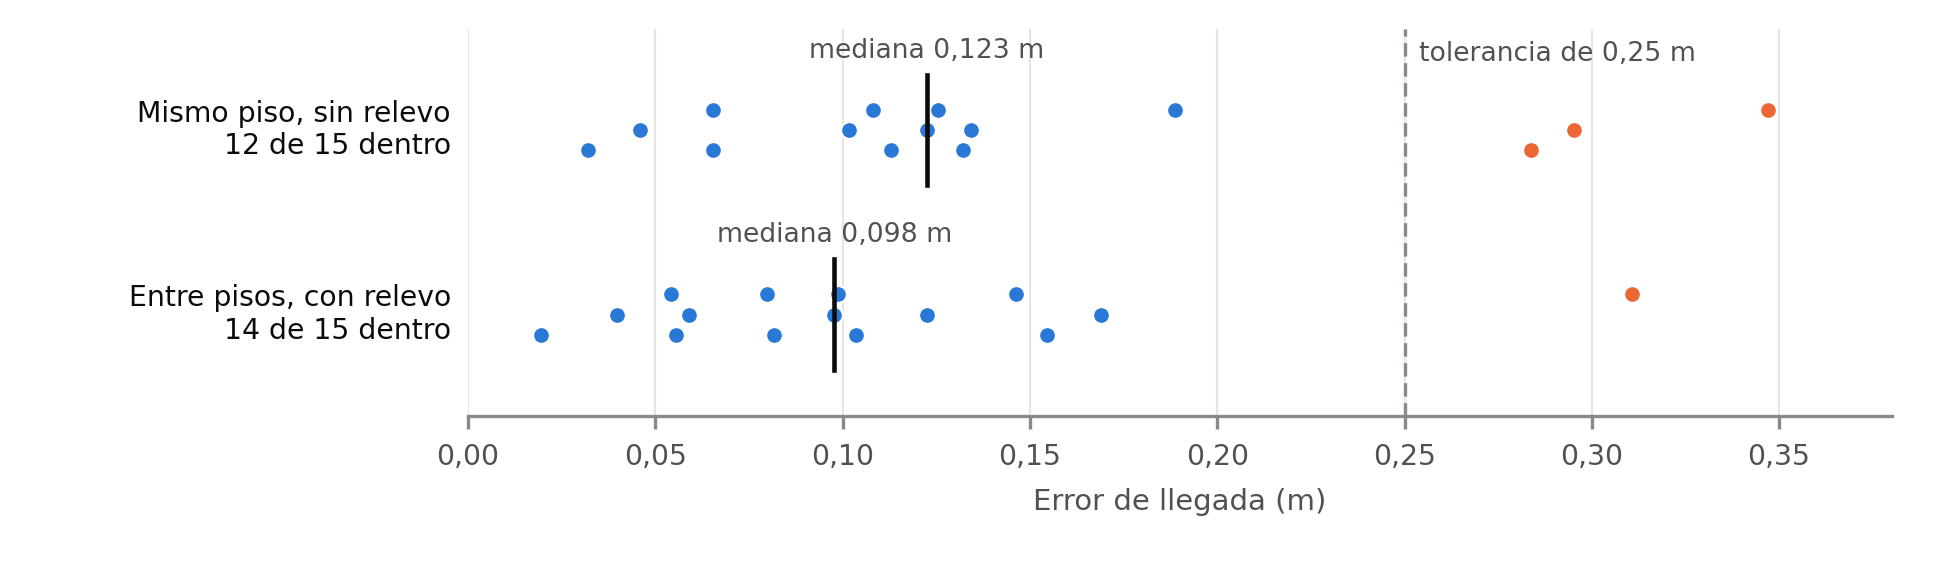
\includegraphics[width=\textwidth]{imagenes/llegada_simulacion.png}
  \caption{Error de llegada de las treinta misiones de la campaña en simulación, por grupo. La línea discontinua es la tolerancia de 0,25~m; en naranja, las cuatro misiones que quedaron fuera de ella. La marca vertical de cada fila es su mediana.}
  \label{fig:llegada-sim}
\end{figure}

\subsection{Tiempo de respuesta y tiempo de asignación}

El tiempo de respuesta se presenta por escalones, sin media ni desviación, debido a una limitación del instrumento (tabla~\ref{tab:respuesta}).

\begin{table}[htbp]
  \caption{Tiempo de respuesta de las treinta misiones, en escalones del reloj de
    la simulación.}
  \label{tab:respuesta}
  \begin{tabular}{@{}lcccc@{}}
    \toprule
    \textbf{Tiempo de respuesta} & 0,1 s & 0,2 s & 0,3 s & 0,4 s \\ \midrule
    Misiones & 10 & 15 & 4 & 1 \\ \bottomrule
  \end{tabular}
\end{table}

Los cuatro valores son múltiplos exactos de 100~ms, el paso con que avanza el reloj de la simulación, y la resolución del instrumento vale entre el 25~\% y el 100~\% de la magnitud medida. Una mediana de 0,2~s significa «uno o dos pasos del reloj», no «doscientos milisegundos», de manera que dar media y desviación sugeriría una precisión que el reloj no entrega. La cota, en cambio, sí se sostiene, y además es lo que le importa a un usuario: el agente arranca en menos de medio segundo.

El tiempo de asignación quedó por debajo de 100~ms en las treinta misiones, varios órdenes de magnitud por debajo de un paso del reloj, razón por la cual se caracterizó aparte, en un banco de pruebas con el reloj del sistema: mediana entre 154 y 175~\textmu s y máximo de 306~\textmu s. La figura~\ref{fig:simulacion} muestra una misión de la campaña.

\begin{figure}[htbp]
  \centering
  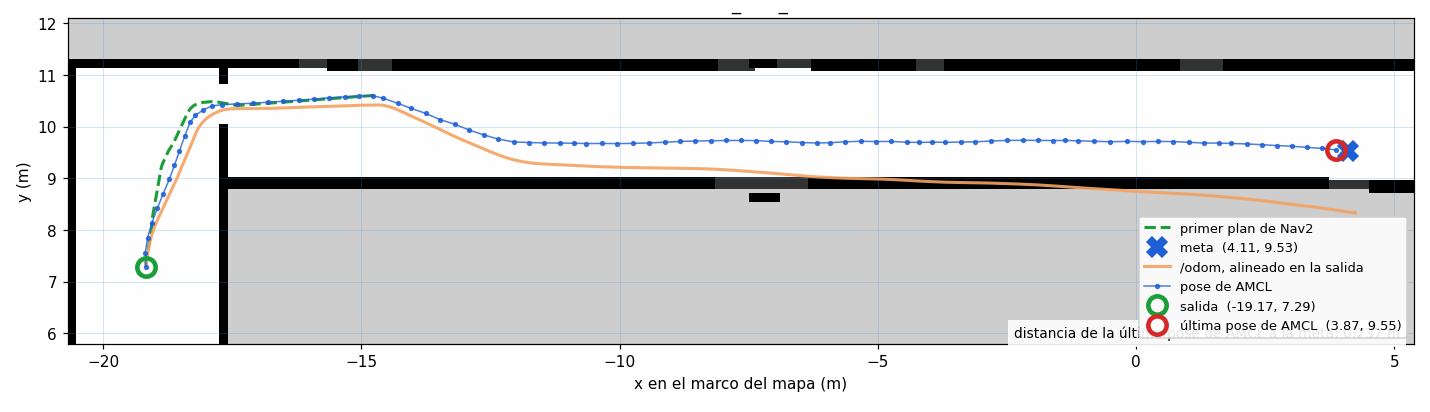
\includegraphics[width=\textwidth]{imagenes/corrida_simulacion.png}
  \caption{Una misión de la campaña en simulación. Se superponen el primer plan
    que calcula el navegador, la pose estimada a lo largo del recorrido y la
    odometría cruda. La separación creciente entre las dos últimas es la deriva
    que la localización corrige contra el mapa.}
  \label{fig:simulacion}
\end{figure}

% ---------------------------------------------------------------------
\section{Evaluación con los agentes físicos}
\label{sec:res-hw}

\subsection{La odometría del agente}

La odometría del agente sale de comparar barridos sucesivos del láser, y entre el 26 de agosto y el 2 de octubre no produjo una medida utilizable. La tabla~\ref{tab:odometria}
reúne lo que se midió en cada entorno, como fracción del avance real medido con
flexómetro.

\begin{table}[H]
  \centering\small
  \caption{Fracción del avance real que registra la odometría, por entorno. El
    criterio de la prueba es un error de 10~\% o menos.}
  \label{tab:odometria}
  \begin{tabular}{@{}p{0.44\textwidth}ccl@{}}
    \toprule
    \textbf{Entorno} & \textbf{Recorrido} & \textbf{Registrado} & \textbf{Criterio} \\ \midrule
    Gregorio, pasillo simulado (46,9 m de extensión en su mapa) & largo & 37,9 \% & no cumple \\
    Gregorio, pasillos simulados de los pisos 2 y 3 & largo & 5,7 \% y 1,3 \% & no cumple \\
    Gregorio, hall del piso 3 & 6 m & 73 \% & no cumple \\
    Cuarto cerrado, desplazado a mano & 3 m & 96,3 -- 101,9 \% & cumple \\
    Catalayud, pasillo del piso 4 & 6,68 m & 95,4 \% & cumple \\
    Catalayud, pasillo del piso 4 & 14,57 m & 103,3 \% & cumple \\
    Catalayud, piso 4, con la unidad inercial & 8,08 m & 101,9 \% & cumple \\
    Catalayud, piso 4, con la unidad inercial & 2,82 m & 104,9 \% & cumple \\ \bottomrule
  \end{tabular}
\end{table}

El estimador es el mismo en todas las filas: lo que cambió fue el entorno. En un pasillo con hornacinas, casilleros y quiebres, con ocho cambios de perfil en 25~m, la odometría queda dentro del $\pm$5~\% sin cambiar un parámetro. Con las dos mediciones del pasillo del piso 4, de 6,68 y 14,57~m, cumplió el criterio de la prueba, del que dependía todo lo demás con los agentes físicos. Las dos últimas filas ya incluyen la unidad inercial; el segundo de esos tramos mide 2,82~m, por debajo de los 5~m que pide el criterio, y se incluye como dato de la misma cadena.

\subsection{La navegación y la precisión de llegada}
\label{sec:res-g3}

La prueba de navegación de un agente pide un recorrido de punto a punto con Nav2 y la llegada verificada con flexómetro, a 0,5~m o menos del destino. En la primera sesión en el piso 4, el 2 de octubre, las dos llegadas medidas quedaron a 0,57 y 0,62~m, cortas, debido a que Nav2 daba entonces la meta por alcanzada a 1,0~m. Con la unidad inercial integrada, ese margen bajó a 0,5~m. El 7 de octubre, uno de los agentes recorrió en el piso 4 tres tramos encadenados, sin que nadie lo tocara entre uno y otro, y después regresó a la salida (tabla~\ref{tab:g3} y figura~\ref{fig:cadena}).

\begin{table}[htbp]
  \centering\small
  \caption{Cadena de tres tramos en el piso 4 y regreso a la salida: llegada de
    cada tramo.}
  \label{tab:g3}
  \begin{tabular}{@{}llcccl@{}}
    \toprule
    \textbf{Tramo} & \textbf{Destino} & \textbf{Tiempo} & \textbf{Recuperaciones} & \textbf{A la meta} & \textbf{Medida} \\ \midrule
    1 & Salón 403 & 13,5 s & 1 & 0,26 m & estimada \\
    2 & Salón 402 & 27,8 s & 1 & 0,45 m & flexómetro \\
    3 & Salón 401 & 5,2 s & 0 & 0,06 m & flexómetro \\
    Regreso & Salida & 62,8 s & 6 & 0,34 m & flexómetro \\ \bottomrule
  \end{tabular}
\end{table}

Las llegadas medidas quedaron dentro de la tolerancia de 0,5~m, y la prueba se superó. La llegada al Salón 403 no se midió porque en ese momento no había flexómetro, y se estimó con el error de los otros dos tramos. El regreso a la salida incluyó una media vuelta en el tramo ancho frente a los salones, que Nav2 resolvió con seis recuperaciones.

\begin{figure}[htbp]
  \centering
  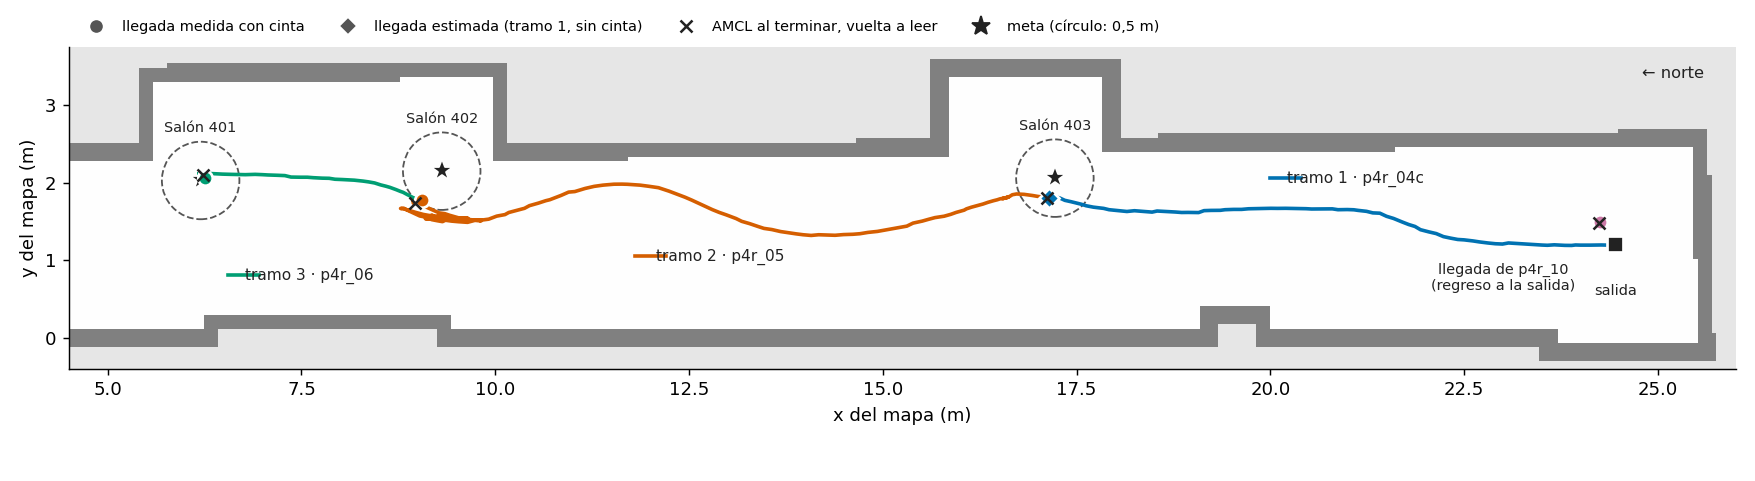
\includegraphics[width=\textwidth]{imagenes/cadena_piso4.png}
  \caption{Cadena de tres tramos en el piso 4 y regreso a la salida: recorrido
    según la localización, llegadas medidas con flexómetro, la llegada estimada
    al Salón 403 y la pose de la localización al terminar cada tramo.}
  \label{fig:cadena}
\end{figure}

El 8 de octubre, el otro agente recorrió el piso 3 en cinco tramos encadenados, con dos medias vueltas entre ellos, y los cinco terminaron con éxito y sin recuperaciones. Esas llegadas no se midieron con flexómetro, y al forzar a la localización a recalcular su pose al final de cada tramo, esta se desplazó entre 0,61 y 0,86~m. La pose que publica la localización al detenerse el agente va atrasada, por lo que la llegada que vale es la medida con flexómetro. La precisión de llegada sigue condicionada por la banda muerta de tracción, ya que el agente se aproxima a la meta a 0,40~m/s y no tiene régimen de aproximación fina.

% ---------------------------------------------------------------------
\section{Evaluación del sistema completo con los agentes físicos}
\label{sec:res-completo}

El 16 de octubre, el sistema completo funcionó con los dos agentes físicos (anexo A, video 7). La misión con relevo del Salón 302 al Salón 402 se completó, y de las diez misiones sorteadas para la campaña, las nueve que llegaron a ejecutarse se completaron, todas con relevo. La décima quedó interrumpida porque el computador portátil se apagó por falta de batería.

\subsection{Condiciones de las pruebas}

Las pruebas se hicieron en los pisos 3 y 4 del edificio Catalayud, con un agente en cada piso. El coordinador y el grabador se ejecutaron en el portátil, y cada misión se pidió desde la página web en un teléfono conectado a la red de los agentes. Los autores hicieron de usuario: pidieron cada misión, acompañaron a los agentes y confirmaron el cambio de piso en la página. Los agentes no se reubicaron entre misiones, y cuando el destino quedaba detrás del agente, el coordinador pidió la media vuelta en varios tiempos. La llegada se verificó con la localización de cada agente, sin medida con flexómetro.

\subsection{La misión con relevo}

La primera prueba del sistema completo fue una misión del Salón 302, en el piso 3, al Salón 402, en el piso 4, que se completó en 132,5~s, con un relevo y con la llegada a 0,444~m del destino. Entre la llegada del primer agente a la escalera y el arranque del segundo pasaron 61,1~s. Fue el segundo intento: en el primero, el coordinador rechazó la llegada del agente del piso 3 al Salón 302, adonde iba a recoger al usuario, porque su localización lo situaba a 0,59~m del punto.

Esa sesión sirvió de ensayo del montaje, y en ella las misiones se eligieron sin seguir el sorteo, de modo que no forman parte de la campaña. De las doce misiones grabadas, siete se completaron y cinco terminaron fallidas: en cuatro, el coordinador rechazó una llegada con el agente a entre 0,51 y 0,78~m del punto, y en la otra Nav2 abortó la navegación.

\subsection{La campaña con las misiones sorteadas}

Las diez misiones de la campaña se sortearon antes de ejecutarlas, con una semilla fija, entre los puntos de interés de los dos pisos: cinco de subida y cinco de bajada. Se ejecutaron en el orden del sorteo, y la tabla~\ref{tab:campana-vehiculos} da el resultado de las nueve que llegaron a ejecutarse.

\begin{table}[htbp]
  \centering\small
  \caption{Campaña con los agentes físicos: las nueve misiones sorteadas que se
    ejecutaron, todas completadas con un relevo. La llegada es la de la
    localización del agente, con una tolerancia de 0,5~m.}
  \label{tab:campana-vehiculos}
  \begin{tabular}{@{}cllccc@{}}
    \toprule
    \textbf{N.\textsuperscript{o}} & \textbf{Origen} & \textbf{Destino} & \textbf{Tiempo total} & \textbf{Respuesta} & \textbf{Llegada} \\ \midrule
    1 & Ascensor, piso 3 & Salón 403 & 52,3 s & 0,51 s & 0,435 m \\
    2 & Salón 302 & Salón 401 & 90,1 s & 0,27 s & 0,202 m \\
    3 & Salón 401 & Salón 302 & 87,6 s & 3,90 s & 0,143 m \\
    4 & Salón 403 & Salón 303 & 78,9 s & 1,25 s & 0,420 m \\
    5 & Salón 402 & Salón 301 & 105,4 s & 0,66 s & 0,285 m \\
    6 & Salón 301 & Salón 401 & 89,8 s & 2,97 s & 0,226 m \\
    7 & Ascensor, piso 4 & Salón 301 & 81,7 s & 0,87 s & 0,234 m \\
    8 & Salón 302 & Salón 403 & 81,8 s & 0,95 s & 0,214 m \\
    9 & Salón 303 & Salón 402 & 92,6 s & 0,63 s & 0,299 m \\ \midrule
    \multicolumn{3}{@{}l}{Mediana} & 87,6 s & 0,87 s & 0,234 m \\ \bottomrule
  \end{tabular}
\end{table}

Con nueve éxitos en nueve misiones, el intervalo de Wilson al 95~\% va del 70,1 al 100~\%, lo que permite afirmar que la tasa de éxito con los agentes físicos supera el 70~\%, la misma cota que sostiene la campaña en simulación. Con la expresión de la norma ASTM F3244-21, nueve repeticiones sin fallo demuestran una fiabilidad mínima de 0,81 con un 85~\% de confianza.

El error de llegada tuvo una mediana de 0,234~m y fue de 0,143 a 0,435~m. El tiempo total, desde la solicitud hasta la llegada verificada, tuvo una mediana de 87,6~s y fue de 52,3 a 105,4~s. El tiempo de respuesta, desde que el coordinador acepta la solicitud hasta que el agente asignado empieza a moverse, tuvo una mediana de 0,87~s y quedó por debajo de 1,3~s en siete de las nueve misiones. Los dos valores más altos, 3,90 y 2,97~s, son de misiones en que el agente ya estaba en el punto de origen: el coordinador verificó esa llegada, que no exigía moverse, con la espera de 1,5~s, y el primer movimiento fue la media vuelta hacia la escalera. El tiempo de asignación fue de 0,3~ms en las nueve misiones, medido con el reloj del portátil e incluyendo el paso del mensaje hasta el grabador, del mismo orden que el del banco de pruebas. En las nueve misiones los agentes hicieron 24 medias vueltas, de entre 160 y 171$^\circ$, en uno a cuatro tiempos cada una.

La figura~\ref{fig:campana-vehiculos} descompone el tiempo de cada misión en sus etapas. Ir a recoger al usuario tomó entre 2,2 y 30,6~s, según dónde había terminado la misión anterior, mientras que el guiado en el piso de origen tuvo una mediana de 24,2~s, y el guiado en el piso de destino, de 24,8~s.

\begin{figure}[htbp]
  \centering
  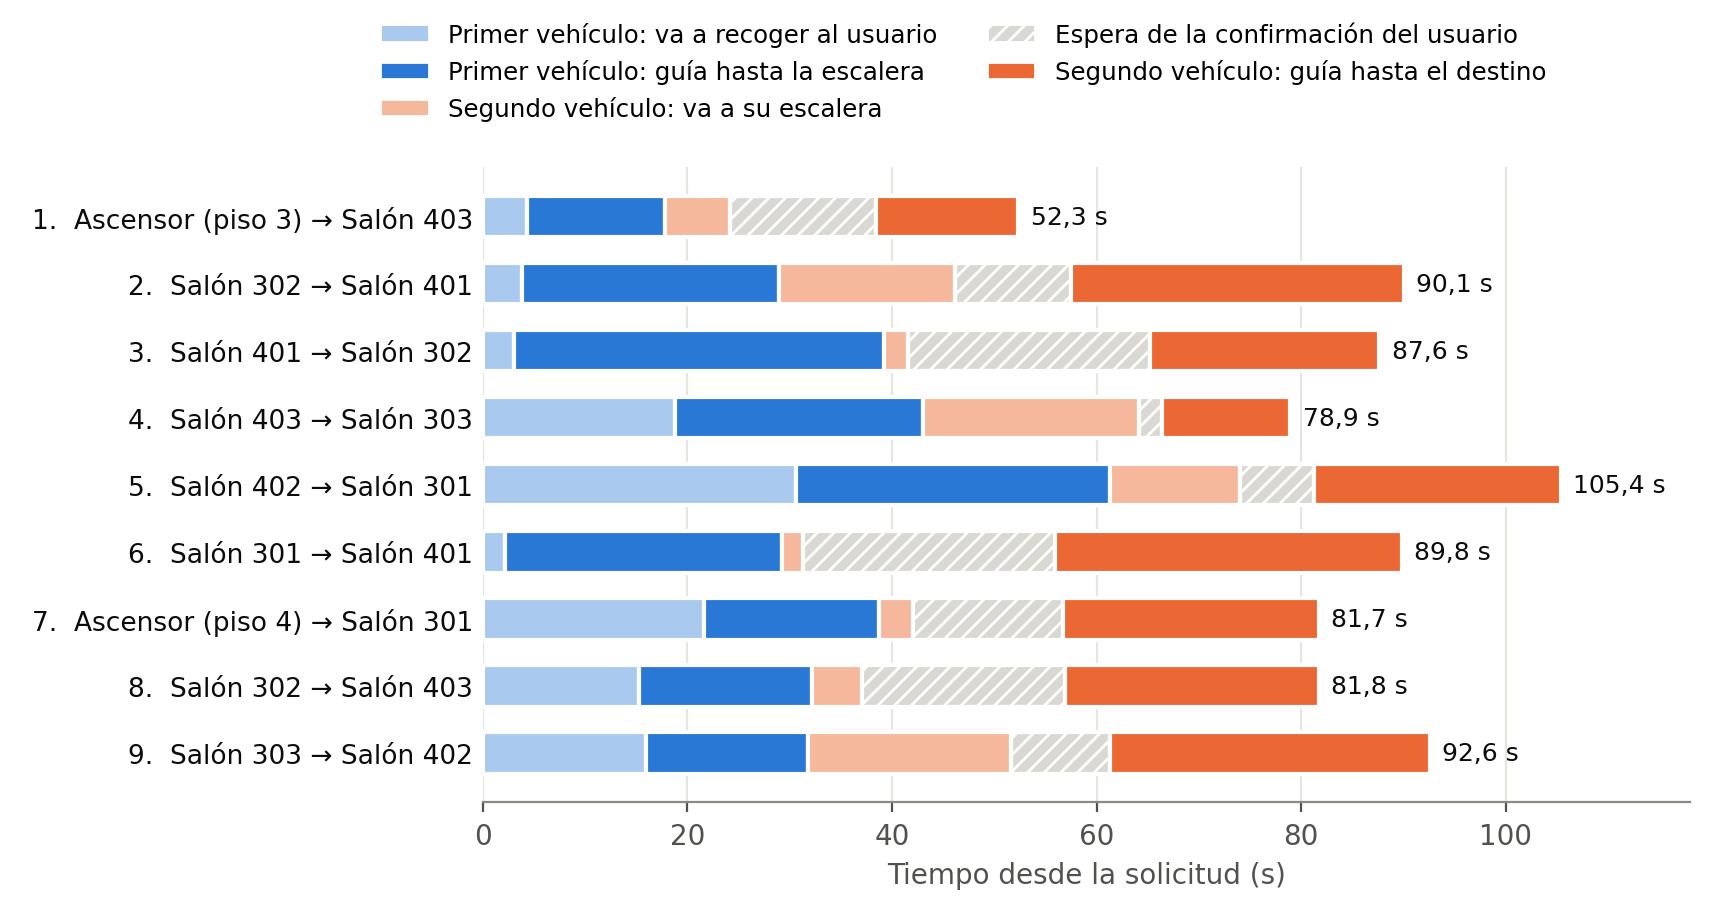
\includegraphics[width=\textwidth]{imagenes/campana_vehiculos_etapas.png}
  \caption{Duración de cada etapa en las nueve misiones de la campaña con los agentes físicos, según las marcas de etapa del coordinador. El tramo rayado es la
    espera de la confirmación de cambio de piso, contada desde que el segundo
    agente está en su escalera.}
  \label{fig:campana-vehiculos}
\end{figure}

\subsection{El relevo entre los dos agentes}

En las nueve misiones el relevo se produjo y el coordinador no pasó por el estado inactivo ni quedó sin agente asignado, aunque, como en simulación, ese criterio no puede fallar por la forma en que está construido. La medida que informa es el intervalo del relevo: el tiempo desde que el primer agente llega a su escalera hasta el primer movimiento del segundo.

Ese intervalo tuvo una mediana de 1,22~s, pero la cifra junta dos situaciones. En cinco misiones el segundo agente tuvo que desplazarse hasta su escalera, en cuatro desde el destino de la misión anterior y en una para corregir su posición, y arrancó en menos de 1,3~s. En las otras cuatro ya estaba en la escalera, su primer movimiento fue el del guiado final, después de la confirmación, y el intervalo, de 12,9 a 27,5~s, mide sobre todo cuánto tardó el usuario en confirmar.

Para el usuario, el tiempo que importa es el que pasa entre la llegada a la escalera del piso de origen y el arranque del guiado en el piso de destino, durante el cual cambia de piso, el segundo agente llega a su escalera si no estaba allí, y el usuario confirma en la página. Ese tiempo tuvo una mediana de 24,8~s y fue de 18,0 a 29,5~s. La confirmación, desde que el segundo agente estaba en su escalera, tomó entre 2,3 y 24,7~s, y el aviso de los 60~s no llegó a mostrarse en ninguna misión.

\subsection{Criterio de conteo e incidencias}

En la tasa de éxito cada misión cuenta una sola vez, con el intento que se completó, mientras que el protocolo cuenta como fallo toda ejecución fallida. Por esa razón conviene declarar los intentos que la tasa deja fuera. Después de reiniciar las cadenas de navegación, las misiones 1 y 2 se completaron al segundo intento. Los dos intentos fallidos ocurrieron en el tramo en que el agente del piso 3 iba a recoger al usuario: en el de la misión 1, el coordinador rechazó la llegada al ascensor, con el agente a 0,526~m del punto, y en el de la misión 2 no tenía la pose del agente para verificar la llegada. En los dos casos el coordinador actuó como estaba previsto, y lo que faltó fue la precisión o la pose del agente.

Antes de esos intentos, la navegación de los dos agentes dejó de responder, y ocho intentos de la misión 1 terminaron rechazados o abortados, con las transformadas de posición detenidas dentro de Nav2. La detención ocurrió después de que el portátil se apagara por falta de batería, con los agentes ya con horas encendidos y con cargas de 10 a 14 en procesadores de dos núcleos. Se reiniciaron las cadenas de navegación con la pose de salida, y después las nueve misiones se ejecutaron sin tocar los agentes.

La misión 10 empezó y no terminó, pues el portátil volvió a apagarse por falta de batería poco después de pedirla, cuando el agente del piso 4 ya había llegado a su escalera. Antes se había pedido por error el ascensor del piso 4 como destino, debido a que los ascensores de los dos pisos aparecían en la página con el mismo nombre; ese intento no es una misión del sorteo y no se cuenta. Después de la campaña, la página muestra el piso junto a los nombres que se repiten.

% ---------------------------------------------------------------------
\section{Limitaciones de la medición}
\label{sec:limitaciones}

\subsection{Naturaleza del criterio de continuidad entre niveles}

La continuidad del servicio es la variable de respuesta principal del cuarto objetivo, y su criterio binario se cumplió en las treinta misiones. Ese resultado, sin embargo, no es evidencia: el criterio exige que, dentro de la ventana de la misión, el coordinador nunca esté inactivo ni tenga el agente sin asignar, y los dos únicos puntos del código que producen esos valores ocurren antes de que la ventana se abra. Como no existe ejecución posible que lo incumpla, el criterio no puede dar un resultado negativo y no aporta evidencia, por muchas veces que se verifique.

No se corrigió inventando una ruta de fallo, ya que eso habría sido instrumentar el experimento para que pareciera más informativo. La continuidad se declaró como un invariante estructural del diseño, y la afirmación se apoyó en una magnitud que sí varía: el intervalo del relevo, entre el final del tramo de un agente y el inicio del tramo del otro. En las quince misiones entre pisos tuvo una mediana de 0,1~s y un máximo de 0,2~s, es decir, uno o dos pasos del reloj de la simulación.

\subsection{Espacio desconocido marcado como libre en el mapa}

El mapa de ocupación es una imagen en la que cada celda es libre, ocupada o desconocida, y su archivo de configuración fija el umbral por debajo del cual una celda se carga como libre. En el mapa de la campaña en simulación ese umbral era 0,25, y las celdas desconocidas, que el formato guarda con una ocupación de 0,196, quedaban por debajo de él. Al cargar el mapa, 10\,908 celdas que el modelo no describía, el 14,5~\% del mapa, se leyeron como espacio libre. Con eso, las dos protecciones que impiden planificar por espacio desconocido, la del planificador y la del mapa de costos, no tenían nada que rechazar.

El defecto no cambia el veredicto de la campaña, puesto que los cuatro fallos fueron de precisión de llegada, sin relación con el trazado, y el pasillo por el que se navegó es libre en el mundo simulado. Queda sin verificar que ninguna trayectoria cruzara una de esas celdas, algo que se puede comprobar con los registros conservados. El umbral se corrigió a 0,10 el 25 de septiembre, después de la campaña.

\subsection{La llegada en los agentes físicos, sin medida externa}
\label{sec:lim-llegada}

En la campaña con los agentes físicos la llegada no tuvo una medida independiente del sistema. El protocolo la toma con flexómetro sobre marcas en el piso, y en esa sesión no se midió, aunque la odometría y la llegada ya se habían verificado con flexómetro en los mismos pisos, en las pruebas de odometría y de navegación. El error que se informa es el de la localización del propio agente contra el punto del catálogo, leído 1,5~s después de que Nav2 diera la meta por alcanzada, con el agente ya detenido. Es la medida con que el coordinador acepta la llegada, así que el sistema verificó su llegada con su propia estimación, que es lo que la regla principal del protocolo procura evitar. Los registros lo declaran con la procedencia de la medida, y el programa de análisis lo advierte al calcular las métricas.

La única comparación entre la localización y el flexómetro en los agentes físicos es la de la cadena de tres tramos en el piso 4, donde la localización, leída de nuevo al terminar cada tramo, quedó a 0,10~m o menos de la medida en el sentido del avance y a 5~cm o menos de lado. En el piso 3, en cambio, forzar a la localización a recalcular su pose al final de cada tramo la desplazó entre 0,61 y 0,86~m. Por lo tanto, el resultado de la campaña se lee así: cada agente, según su propia localización, llegó a menos de 0,5~m del destino, y queda sin medir si la distancia real cumplió la misma tolerancia.

% =====================================================================
%  CONCLUSIONES (versión de revisión, se compila con main_revision.tex)
%
%  Correcciones del 4 de noviembre. Un párrafo por objetivo específico, que es lo
%  que pide la plantilla. Cada uno dice lo obtenido, su causa y lo que implica.
%  No se mencionan defectos ya corregidos ni se repite lo que el documento ya dijo.
% =====================================================================
\chapter*{Conclusiones}
\addcontentsline{toc}{chapter}{CONCLUSIONES}

Al modelar la arquitectura funcional se comprobó que el cambio de piso puede
resolverse como un problema de coordinación, sin que ningún agente suba escaleras ni
use el ascensor. En ninguna misión de las dos campañas falló la asignación ni el
relevo, y a ello contribuyó escribir la planificación sin dependencia de ROS~2, lo que
permitió probar todas las combinaciones de origen y destino sin usar el simulador. Con
un solo agente admisible por piso, la asignación resulta trivial; la dificultad y el aporte del trabajo están en coordinar dos agendas que dependen una de otra durante el relevo.

La plataforma AWS DeepRacer sirve como agente de guiado en interiores, pero su
desempeño depende del sitio y de la tracción. Al no tener codificadores en las ruedas,
su avance solo puede medirse donde el pasillo ofrece estructura al láser: en el
edificio Gregorio la odometría registró como máximo el 73~\% del avance real, mientras
que en Catalayud, con el mismo estimador, cumplió el criterio de la prueba. El sitio de operación debe elegirse como parte del diseño. Por debajo de 0,40~m/s la
tracción no responde, por lo que el agente no tiene una aproximación fina y la
tolerancia de llegada tuvo que fijarse en 0,5~m, el doble de la admitida en simulación.
Con una tarjeta de dos núcleos fue necesario llevar la coordinación a un computador
portátil, y la duración de las sesiones queda limitada por las baterías, que en las pruebas se agotaron en los agentes y en ese computador.

Para operar el sistema basta una página web servida en la red local: en las pruebas
con los agentes físicos cada misión se pidió, se siguió y se confirmó desde un
teléfono, sin instalar nada y sin salida a internet. Sin embargo, las funciones que más
la acercan a una operación real no estaban en el anteproyecto y se añadieron al ver el
sistema en uso. Gracias a la confirmación de cambio de piso, una misión no se da por
completada con el usuario en el piso equivocado, un caso que la instrumentación habría
registrado como éxito, y la cancelación devolvió al agente a su escalera en las seis
misiones canceladas. Por lo tanto, los requisitos de una interfaz como esta no pueden cerrarse de antemano.

Con la evaluación experimental se puede afirmar, con 95~\% de confianza, que la tasa de
éxito del sistema supera el 70~\%, tanto en las treinta misiones en simulación como en
las nueve con los agentes físicos, aunque esas muestras no permiten precisar cuánto la
supera. En ese último caso, la cota se apoya en la localización del propio agente, pues la
llegada no se midió con flexómetro. Como todos los fallos fueron de navegación, sobre
todo de precisión de llegada, y ninguno de asignación ni de relevo, la mejora del
sistema pasa primero por la navegación.

% =====================================================================
%  TRABAJOS FUTUROS
%
%  Revisión del 27 de octubre: las cinco líneas que pidieron los autores
%  (navegación, cómputo, evasión de obstáculos, otro controlador e interacción
%  por voz). Las seis anteriores, de campañas más grandes a evaluación con
%  usuarios, se quitaron por indicación de los autores. El 3 de noviembre, también
%  a pedido de los autores, se añadió la de más agentes y misiones simultáneas, que
%  el marco teórico deja anunciada.
% =====================================================================
\chapter*{Trabajos futuros}
\addcontentsline{toc}{chapter}{TRABAJOS FUTUROS}

\paragraph{Una navegación más precisa.} La navegación de los agentes se puede
mejorar en dos frentes. El primero es la tracción: el agente no se mueve por
debajo de 0,40~m/s, de modo que calibrar el variador o cambiar la relación de transmisión
le daría el régimen lento que hoy le falta para la aproximación final. El
segundo es la medida del avance: codificadores en las ruedas, u odometría visual
con las cámaras que el agente ya lleva, darían una medida que no depende de que
el pasillo tenga estructura. Con las dos, la tolerancia de llegada podría volver
a 0,25~m y el sistema dejaría de depender del entorno para localizarse.

\paragraph{Más capacidad de cómputo.} La tarjeta original, de dos núcleos,
queda entre el 54 y el 59~\% de uso en reposo con la navegación completa, y su
carga se dispara cuando los procesos de los dos agentes se anuncian en la red.
Adaptar la plataforma a una Raspberry Pi~4 o~5, de cuatro núcleos, daría margen
para la navegación, para un controlador más exigente y para la evasión de
obstáculos. Para la Raspberry Pi~4, la comunidad de AWS DeepRacer ya publica el
software de la plataforma.

\paragraph{Evasión de obstáculos.} Las pruebas se hicieron con los pasillos
despejados. En un edificio en uso, el agente tiene que esquivar a las personas
que se cruzan y los objetos que cambian de sitio, y no solo detenerse ante
ellos. Integrar la evasión de obstáculos en movimiento, y probarla con
personas que caminan por el pasillo, es el paso previo a operar en horario de
clases.

\paragraph{Más agentes y misiones simultáneas.} El sistema atiende una misión a la
vez, con un solo agente por piso, y con esas dos condiciones la asignación es
trivial. Con dos o más agentes elegibles por tarea, o con varias solicitudes a la
vez, harían falta una cola de solicitudes, la noción de agente ocupado y un método
que decida entre candidatos, como el húngaro o una subasta. Es la extensión natural
del trabajo para edificios con más afluencia, y obliga a medir de nuevo el costo del
descubrimiento en la red, que crece con el número de procesos.

\paragraph{Un controlador predictivo.} El seguimiento de trayectorias usa
Regulated Pure Pursuit, que sigue la ruta punto a punto y cuya protección de
seguridad anula la curvatura cuando una inversión de marcha queda cerca de la
meta. Un controlador predictivo, como el MPPI que incluye Nav2 y que admite
cinemática tipo automóvil, optimiza el movimiento varios pasos hacia adelante y
tiene en cuenta los obstáculos. Con él, la media vuelta podría volver a Nav2 y
la aproximación final sería más precisa. Como exige más cómputo, va de la mano de la línea anterior.

\paragraph{Interacción por voz.} La interfaz pide elegir el origen y el destino
en listas. Con reconocimiento de voz a texto y un modelo de lenguaje, el usuario
podría pedir el servicio hablando, por ejemplo «lléveme al Salón 402», y el
sistema le explicaría cada etapa en voz alta. Como la red del edificio puede no
tener salida a internet, los dos modelos tendrían que ejecutarse en el computador del coordinador. El de lenguaje solo traduciría la petición a un origen y un
destino del catálogo, sin decidir el recorrido, que sigue a cargo del
planificador.


% =====================================================================
%  REFERENCIAS
% =====================================================================
\ustaseccion{Referencias bibliográficas}
\printbibliography[heading=none]

% =====================================================================
%  ANEXOS
% =====================================================================
% =====================================================================
%  ANEXOS
%  Anexo A, añadido el 27 de octubre de 2026 a pedido de los autores: los
%  videos del proyecto publicados en el canal de YouTube de Santiago
%  Hernández, en orden de publicación. Están «no listados» (se abren con
%  el enlace) salvo el primero, que es público. Los otros videos del canal
%  son de otras asignaturas y no entran. La descripción de cada uno sigue la
%  de su entregable semanal o la del sitio del proyecto.
%  Anexo B, añadido el mismo día: el repositorio, con toda la trazabilidad.
%  Anexo C, añadido el 5 de noviembre a pedido de los autores: el grafo real de nodos, como archivo
%  aparte porque no se leería en una página.
% =====================================================================
\chapter*{Anexo A. Videos del proyecto}
\addcontentsline{toc}{chapter}{ANEXO A. VIDEOS DEL PROYECTO}

Videos publicados en YouTube durante el proyecto, en orden de publicación. Cada
código QR abre el video correspondiente.

\begin{table}[H]
  \centering\small
  \renewcommand{\arraystretch}{1.0}
  \begin{tabular}{@{}c >{\raggedright\arraybackslash}p{0.13\textwidth} p{0.52\textwidth} c c@{}}
    \toprule
    \textbf{N.\textsuperscript{o}} & \textbf{Publicado} & \textbf{Contenido} & \textbf{Duración} & \textbf{Enlace} \\ \midrule
    1 & 5 may. 2026 & El agente en el modelo simulado del pasillo de la universidad, con el seguidor de paredes. \newline \url{https://youtu.be/Q0w_CTga98k} & 1:12 & \raisebox{-0.85\height}{\qrcode[height=1.25cm]{https://youtu.be/Q0w_CTga98k}} \\ \addlinespace
    2 & 19 may. 2026 & Teleoperación del agente en el modelo del piso 2 del edificio Gregorio, con la respuesta de los sensores y el mapeo en RViz. \newline \url{https://youtu.be/ZPJ0Qw2L5-A} & 1:00 & \raisebox{-0.85\height}{\qrcode[height=1.25cm]{https://youtu.be/ZPJ0Qw2L5-A}} \\ \addlinespace
    3 & 5 ago. 2026 & Liberación y prueba de marcha del AWS DeepRacer desde su interfaz web. \newline \url{https://youtu.be/ZGfAMnC4lYY} & 0:44 & \raisebox{-0.85\height}{\qrcode[height=1.25cm]{https://youtu.be/ZGfAMnC4lYY}} \\ \addlinespace
    4 & 18 ago. 2026 & Media vuelta en simulación con Nav2: la meta queda detrás del agente y el planificador la resuelve con una inversión de marcha, vista en Gazebo y en RViz. \newline \url{https://youtu.be/6SABSgCxVEw} & 0:47 & \raisebox{-0.85\height}{\qrcode[height=1.25cm]{https://youtu.be/6SABSgCxVEw}} \\ \addlinespace
    5 & 24 ago. 2026 & Primeras asignaciones de destinos desde el coordinador, con un agente y Nav2 en simulación. \newline \url{https://youtu.be/iKYSiM9cs-Y} & 0:45 & \raisebox{-0.85\height}{\qrcode[height=1.25cm]{https://youtu.be/iKYSiM9cs-Y}} \\ \addlinespace
    6 & 5 sep. 2026 & Campaña de treinta misiones sorteadas en simulación, con los dos agentes y el coordinador. \newline \url{https://youtu.be/eH_Co4vZZdw} & 3:48 & \raisebox{-0.85\height}{\qrcode[height=1.25cm]{https://youtu.be/eH_Co4vZZdw}} \\ \addlinespace
    7 & 20 oct. 2026 & Campaña con los agentes físicos en los pisos 3 y 4 del edificio Catalayud: misiones con relevo pedidas, seguidas y confirmadas desde un teléfono. \newline \url{https://youtu.be/X3BINGgNxiA} & 12:40 & \raisebox{-0.85\height}{\qrcode[height=1.25cm]{https://youtu.be/X3BINGgNxiA}} \\
    8 & 1 nov. 2026 & Ajustes de la página y cancelación de misiones con los agentes físicos, con la pantalla del teléfono sincronizada. \newline \url{https://youtu.be/31oNn04qLoU} & 8:21 & \raisebox{-0.85\height}{\qrcode[height=1.25cm]{https://youtu.be/31oNn04qLoU}} \\ \bottomrule
  \end{tabular}
\end{table}

\chapter*{Anexo B. Repositorio del proyecto}
\addcontentsline{toc}{chapter}{ANEXO B. REPOSITORIO DEL PROYECTO}

El repositorio público del proyecto guarda toda su trazabilidad. Contiene el
código de los agentes, del coordinador y de la interfaz; la matriz de requisitos,
con la prueba que declara cumplido cada uno; el protocolo experimental; el
registro de cada misión de las dos campañas y el programa que calcula las
métricas; la evidencia de cada sesión de trabajo, con sus mediciones; los
entregables semanales y la bitácora del proyecto. El sitio del proyecto presenta
el mismo contenido para leerlo en el navegador.

\begin{table}[H]
  \centering\small
  \renewcommand{\arraystretch}{1.3}
  \begin{tabular}{@{}p{0.2\textwidth} p{0.56\textwidth} c@{}}
    \toprule
    \textbf{Recurso} & \textbf{Dirección} & \textbf{Código} \\ \midrule
    Repositorio & \url{https://github.com/shdeza12/Collaborative-Mobile-Robot-System-for-Indoor-Navigation-Assistance-in-Multi-Level-Environments} & \raisebox{-0.85\height}{\qrcode[height=2cm]{https://github.com/shdeza12/Collaborative-Mobile-Robot-System-for-Indoor-Navigation-Assistance-in-Multi-Level-Environments}} \\ \addlinespace
    Sitio del proyecto & \url{https://shdeza12.github.io/Collaborative-Mobile-Robot-System-for-Indoor-Navigation-Assistance-in-Multi-Level-Environments/} & \raisebox{-0.85\height}{\qrcode[height=2cm]{https://shdeza12.github.io/Collaborative-Mobile-Robot-System-for-Indoor-Navigation-Assistance-in-Multi-Level-Environments/}} \\ \bottomrule
  \end{tabular}
\end{table}

\chapter*{Anexo C. Grafo de nodos del sistema}
\addcontentsline{toc}{chapter}{ANEXO C. GRAFO DE NODOS DEL SISTEMA}

Grafo de nodos y tópicos de ROS~2 obtenido con el generador de la herramienta \texttt{rqt\_graph} el 5 de noviembre de 2026, con el sistema completo en simulación en los pisos 3 y 4 del edificio Catalayud: los dos agentes, el coordinador, el grabador y el puente de la página, durante una misión con relevo pedida y confirmada desde la página, que se completó en 99,0~s. Reúne 69 nodos, así que se consulta como archivo aparte, que se puede ampliar sin perder detalle.

La captura se hizo en simulación debido a que, con los agentes físicos, el portátil solo admite cuatro procesos de ROS~2 durante una misión, y el láser y las transformadas no salen de cada agente. De ahí que no aparezcan los nodos propios de los agentes físicos, como la odometría del láser, la unidad inercial, el filtro y el puente a los servos, que sí muestra la figura~\ref{fig:nodos}.

\begin{table}[H]
  \centering\small
  \renewcommand{\arraystretch}{1.3}
  \begin{tabular}{@{}p{0.2\textwidth} p{0.56\textwidth} c@{}}
    \toprule
    \textbf{Recurso} & \textbf{Dirección} & \textbf{Código} \\ \midrule
    Grafo de nodos, en PDF & \url{https://github.com/shdeza12/Collaborative-Mobile-Robot-System-for-Indoor-Navigation-Assistance-in-Multi-Level-Environments/blob/main/Documentos/Evidencia/S30_grafo_rqt.pdf} & \raisebox{-0.85\height}{\qrcode[height=2cm]{https://github.com/shdeza12/Collaborative-Mobile-Robot-System-for-Indoor-Navigation-Assistance-in-Multi-Level-Environments/blob/main/Documentos/Evidencia/S30_grafo_rqt.pdf}} \\ \bottomrule
  \end{tabular}
\end{table}


\end{document}
